\documentclass[dvipsnames,table]{include/thesisclass} %compile with lualatex
\usepackage{media9}
%\usepackage[dvipsnames,table]{xcolor} %option clash with media9

\usepackage{listings}
\usepackage{float}
\usepackage{pdfpages}
\usepackage{subcaption}

%for tables
\usepackage{tabularx}
\usepackage{dcolumn,booktabs}
\renewcommand\thempfootnote{\arabic{mpfootnote}}
\newcolumntype{d}[1]{D{.}{.}{#1}}
\newcommand\mc[1]{\multicolumn{1}{c}{#1}} % handy shortcut macro

%misc
\usepackage{siunitx}
\sisetup{range-phrase=--} %used for \SIrange{1}{2}{\volt}
\DeclareSIUnit{\sample}{S}
\DeclareSIUnit{\bits}{B}
\usepackage{nicefrac}
\usepackage{amsmath}
\usepackage[normalem]{ulem}
\usepackage[figuresright]{rotating}
\usepackage{lscape}
\usepackage{textcomp}
\usepackage{trfsigns}
\usepackage{enumitem}
\newcommand{\thz}{\si{\tera\hertz}}
\newcommand{\eqdev}{\mathrel{\widehat{=}}}

%tikz & pgfplots
\usepackage{wrapfig}
\usepackage{tikz,tikzscale,pgfplots,pgfplotstable,circuitikz,tikz-timing}
\usetikzlibrary{arrows,shapes,shadows,external,decorations.pathmorphing, positioning}
\tikzexternalize[optimize=false,prefix=tikz/]
\usetikztiminglibrary{arrows, clockarrows, nicetabs}
\pgfplotsset{compat=1.11}

\usetikzlibrary{fadings}
\tikzfading %strangely gives bad bounding box when inside the tikzpicture
[
  name=fade out,
  inner color=transparent!0,
  outer color=transparent!100
]


\usepgfplotslibrary{units,fillbetween,colormaps} 
\pgfplotsset{compat=newest}

\pgfdeclarehorizontalshading{visiblelight}{50bp}{
	color(0.00000000000000bp)=(violet);
	color(8.33333333333333bp)=(blue);
	color(16.66666666666670bp)=(cyan);
	color(25.00000000000000bp)=(green);
	color(33.33333333333330bp)=(yellow);
	color(41.66666666666670bp)=(orange);
	color(50.00000000000000bp)=(red)
} 

\lstset{%
	breaklines=true,
	breakatwhitespace=true,
}

\renewcommand{\subsectionautorefname}{\sectionautorefname}
\renewcommand{\subsubsectionautorefname}{\sectionautorefname}




\SelectLanguage{english}
% details on this thesis
\newcommand{\thesisauthor}{Olena Manzhura}
\newcommand{\thesisentopic}{A Terabit Sampling System with a Photonics Time-Stretch ADC}
%\newcommand{\thesisentopic}{Ein Terabit Abtastsystem mit Photonic-Time-Stretch Analog-Digital-Wandler}
\newcommand{\thesislongtopic}{}
\newcommand{\thesisinstitute}{Institute for Data Processing and Electronics (IPE)}
\newcommand{\thesisreviewerone}{Prof. Dr. Anke-Susanne Müller (LAS)}
\newcommand{\thesisreviewertwo}{Dr. Michele Caselle (IPE)}
\newcommand{\thesisadvisorone}{} % to use: enter names and uncomment in titlepg
\newcommand{\thesisadvisortwo}{}
\newcommand{\thesistimestart}{15.11.2020} % on titlepage
\newcommand{\thesistimeend}{13.08.2021} % on titlepage
\newcommand{\thesistimehandin}{13.08.2021} % on second page 'preamble'
\newcommand{\thesispagehead}{Master Thesis: \thesisentopic} % page heading


\let\Oldsection\section
\renewcommand{\section}{\FloatBarrier\Oldsection}
\let\Oldsubsection\subsection
\renewcommand{\subsection}{\FloatBarrier\Oldsubsection}
\let\Oldsubsubsection\subsubsection
\renewcommand{\subsubsection}{\FloatBarrier\Oldsubsubsection}
 
 
\hypersetup
{
    pdfauthor={\thesisauthor},
    pdftitle={Masterarbeit: \thesisentopic},
    pdfsubject={\thesislongtopic},
    pdfkeywords={kit,etit,master,thesis,\thesisauthor}
}
\hyphenation
{
    über-nom-me-nen an-ge-ge-be-nen
}
\DeclareSIUnit{\sample}{S}
\sisetup{per-mode=symbol}

% acronyms
\usepackage[acronym,nomain,toc]{glossaries}
\glstoctrue
\makeglossaries
\newacronym{kit}{KIT}{Karlsruhe Institute of Technology}
\newacronym{sr}{SR}{Synchrotron Radiation}
\newacronym{linac}{LINAC}{linear accelerator}
\newacronym{rf}{RF}{Radio Frequency}
\newacronym{ipe}{IPE}{Institute for Data Processing and Electronics}
\newacronym{kara}{KARA}{Karlsruhe Research Accelerator}
\newacronym{kapture}{KAPTURE}{Karlsruhe Pulse Taking Ultra-fast Readout Electronics}
\newacronym{csr}{CSR}{Coherent Synchrotron Radiation}
\newacronym{eo}{EO}{Electro-Optic}
\newacronym{adc}{ADC}{Analog-To-Digital-Converter}
\newacronym{dac}{DAC}{Digital-To-Analog-Converter}
\newacronym{sha}{SHA}{Sample-And-Hold-Amplifier}
\newacronym{tha}{THA}{Track-And-Hold-Amplifier}
\newacronym{pll}{PLL}{Phase-Locked-Loop}
\newacronym{fmc}{FMC}{FPGA Mezzanine Card}
\newacronym{hspce}{HSPCe}{High Serial Pin Count Extension} 
\newacronym{lvcmos}{LVCMOS}{Low voltage complementary metal oxide semiconductor}
\newacronym{lvds}{LVDS}{Low Voltage Differential Signaling}
\newacronym{lvpecl}{LVPECL}{Low-voltage positive emitter-coupled logic}
\newacronym{pcie}{PCIe}{PCI Express}
\newacronym{theresa}{THERESA}{Terahertz Readout Sampling}
\newacronym{rfsoc}{RFSoC}{Radio-Frequency System-On-Chip}
\newacronym{lsb}{LSB}{Least Significant Bit}
\newacronym{dc}{DC}{Direct Current}
\newacronym{ac}{AC}{Alternating Current}
\newacronym{thz}{THz}{tera Hertz}
\newacronym{fwhm}{FWHM}{Full Width At Half Maximum}
\newacronym{fpga}{FPGA}{Field Programmable Gate Array}
\newacronym{lna}{LNA}{Low-Noise-Amplifier}
\newacronym{daq}{DAQ}{Data Acquisition System}
\newacronym{mmic}{MMIC}{Microwave Monolithic Integrated Circuit}
\newacronym{sinad}{SINAD}{Signal-to-Noise-and-Distortion Ratio}
\newacronym{snr}{SNR}{Signal-To-Noise-Ratio}
\newacronym{inl}{INL}{Integral Nonlinearity}
\newacronym{dnl}{DNL}{Differential Nonlinearity}
\newacronym{sfdr}{SFDR}{Spurious-Free Dynamic Range}
\newacronym{rms}{RMS}{Root-Mean-Square}
\newacronym{rss}{RSS}{Root-Sum-Square}
\newacronym{enob}{ENOB}{Effective-Number-Of-Bits}
\newacronym{dbfs}{dBFS}{decibels relative to full scale}
\newacronym{dbc}{dBc}{decibels relative to the carrier}
\newacronym{sjnr}{SJNR}{Signal-to-Jitter-Noise-Ratio}
\newacronym{pcb}{PCB}{Printed Circuit Board}
\newacronym{spi}{SPI}{Serial Peripheral Interface}
\newacronym{vita}{VITA}{VMEbus International Trade Association}
\newacronym{sma}{SMA}{SubMiniature version A}
\newacronym{fs}{FS}{Full-Scale}
\newacronym{ic}{IC}{Integrated Circuit}
\newacronym{emi}{EMI}{Electro-Magnetic Interference}
\newacronym{cml}{CML}{Current Mode Logic}
\newacronym{sdi}{SDI}{Serial Data Interface}
\newacronym{esr}{ESR}{Equivalent-Series-Resistance}
\newacronym{esl}{ESL}{Equivalent-Series-Inductance}
\newacronym{vcxo}{VCXO}{Voltage-Controlled Crystal Oscillator}




\setcounter{tocdepth}{2}



\begin{document}
    % Titlepage and ToC
    \FrontMatter
    
	\tikzexternaldisable
    % coordinates for background border
\newcommand{\diameter}{20}
\newcommand{\xone}{-15}
\newcommand{\xtwo}{160}
\newcommand{\yone}{15}
\newcommand{\ytwo}{-253}




\begin{titlepage}
    % background border
    \begin{tikzpicture}[overlay]
    \draw[color=gray]
            (\xone mm, \yone mm)
      -- (\xtwo mm, \yone mm)
    arc (90:0:\diameter pt)
      -- (\xtwo mm + \diameter pt , \ytwo mm)
        -- (\xone mm + \diameter pt , \ytwo mm)
    arc (270:180:\diameter pt)
        -- (\xone mm, \yone mm);
    \end{tikzpicture}



    % KIT image and sign for faculty of physics
    \begin{textblock}{10}[0,0](4.5,2.5)
        \includegraphics[width=.25\textwidth]{include/kitlogo.pdf}
    \end{textblock}
    \changefont{phv}{m}{n}    % helvetica
    \begin{textblock}{10}[0,0](5.5,2.2)
        \begin{flushright}
             \large DEPARTMENT OF ELECTRICAL ENGENEERING \\ 
             AND INFORMATION TECHNOLOGY
             \\\thesisinstitute
        \end{flushright}
    \end{textblock}



    % horizontal line
    \begin{textblock}{10}[0,0](4.2,3.1)
        \begin{tikzpicture}[overlay]
        \draw[color=gray]
                (\xone mm + 5 mm, -12 mm)
          -- (\xtwo mm + \diameter pt - 5 mm, -12 mm);
        \end{tikzpicture}
    \end{textblock}



    % begin of text part
    \changefont{phv}{m}{n}    % helvetica
    \centering



    % thesis topic (en and ge)
    \vspace*{3cm}
    \Huge\thesistopic\\
    %\huge(\thesisentopic)\\



    % author name and institute
    \vspace*{2cm}
    \LARGE Master Thesis\\of\\
    \vspace*{1cm}
    \thesisauthor\\
    \vspace*{1cm}
    \LARGE at the \thesisinstitute



    % possible frontimage - thanks to JabberWok
    % for publishing the img under GNU Document License
    \vspace*{1.5cm}
    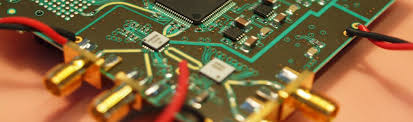
\includegraphics[scale=0.7]{./include/frontimage.png}\\



    % examiners (Referenten)
    \vspace*{1.5cm}
    \LARGE
    \begin{center}
        \begin{tabular}[ht]{l c l}
        \iflanguage{english}{Reviewer}{Referent}: 
            & \hfill & \thesisreviewerone\\
        \iflanguage{english}{Second Reviewer}{Korreferent}: 
            & \hfill & \thesisreviewertwo\\
        % uncomment if you want to provide info on your advisors
        %\iflanguage{english}{Advisor}{Betreuender Mitarbeiter}: 
        %    & \hfill & \thesisadvisorone\\
        %\iflanguage{english}{Second Advisor}{Zweiter betreuender Mitarbeiter}: 
        %    & \hfill & \thesisadvisortwo\\
        \end{tabular}
    \end{center}



    % working time
    \vspace{1cm}
    \begin{center}
        %\large{{Bearbeitungszeit}: 
        \thesistimestart \hspace*{0.25cm} -- %
                                 \hspace*{0.25cm} \thesistimeend
    \end{center}



    % lowest text blocks concerning the KIT
    \begin{textblock}{10}[0,0](2,16.8)
        \tiny{KIT – Die Forschungsuniversität in der Helmholtz-Gemeinschaft}
    \end{textblock}
    \begin{textblock}{10}[0,0](10,16.75)
        \large{\textbf{www.kit.edu}}
    \end{textblock}
\end{titlepage}

    \tikzexternalenable
    \chapter*{Declaration}
I hereby declare that I wrote my master thesis on my own and that I have followed the regulations relating to good scientific practice of the Karlsruhe Institute of Technology (KIT) in its latest form. I did not use any unacknowledged sources or means, and I marked all references I used literally or by content.\\

\vspace{1cm}

\renewcommand{\arraystretch}{0} % for spacing in the tabular environment

\begin{flushright}
	\begin{tabular}{rr}
		Karlsruhe, \thesistimehandin, & \hspace*{5cm}\\[0mm]
		\cline{2-2}\\[2mm]    % the last line has height 2mm due
		& \thesisauthor       % to \arraystretch=0
	\end{tabular}
\end{flushright}

\vfill

\begin{flushright}
	Approved as an exam copy by \\
	\vspace{1cm}
	\begin{tabular}{rr}
		Karlsruhe, \thesistimehandin, & \hspace*{5cm}\\[0mm]
		\cline{2-2}\\[2mm]    % the last line has height 2mm due
		& \thesisreviewerone  % to \arraystretch=0
	\end{tabular}
\end{flushright}

\renewcommand{\arraystretch}{1}

\cleardoublepage

    \chapter*{Abstract}

Analysis of events occurring in the range of femtoseconds is desired in many scientific experiments.
The high temporal resolution needed for measuring such events imposes a great technological challenge for \glspl{daq} and \glspl{adc}.
In order to relax the requirements on the acquisition systems, the so-called optical time-stretch technique is used to stretch the analog input signal in time.
By using this method data converters can be operated at lower sample rate than would be required without it (several \gls{thz} to ). 
Measuring the signal with commercial \glspl{daq}, such as digital storage oscilloscopes, still poses another challenge.
Due to the limited acquisition time windows of such systems, continuous measurements at high sampling rate over a long period of time is not possible.
In applications, where measurements of the long-term evolution of the ultra-fast events with high temporal resolution is necessary, the limited memory size is a large limitation.
Therefore new concepts of \glspl{daq} based on the photonic time-stretch method need to be considered.

In this thesis, a first demonstrator of such a new photonic time-stretch based \gls{daq} system has been developed.
The system consists of a high bandwidth front-end sampling card, mounted on a back-end readout card integrating a new generation of \gls{rfsoc} for readout and processing of the acquired samples. 
%todo photonic time stretch erklären

First, the signal under study is stretched using chirped optical pulses and using the chromatic dispersion in optical fibers.
The signal is measured with a photodetector and sampled by the front-end sampling card.
The front-end sampling card integrates 16 sampling channels, each containing a \gls{tha}. 
The sampling time of these \glspl{tha} can be delayed individually.
In this way the so-called time-interleaving method can be implemented to sample the signal at a higher rate thant that normally possible due to the Nyquist theorem.
The design of the board allows it to be used with the time-stretch method as well as independently from it.
Furthermore, the setup allows for different sampling modes.
In single-channel mode one detector is connected to one sampling channel, therefore allowing to acquire data from up to 16 detectors at the same time with one sampling point per channel.
In the multi-channel mode, several channels are connected to one detector via power-splitter, therefore allowing multiple sampling points for one detector. %todo sample time

The \gls{rfsoc} on the back-end readout card integrates a processing unit and a \gls{fpga}. 
A firmware running on the \gls{fpga} is responsible for programming and controlling the components on the sampling card, as well as collecting the acquired samples and sending it to the following processing system via high-speed connections.
The processing unit, hosting e.g. an operating system or a standalone application, allows for the user to control and monitor the overall system via common periphery, e.g. Ethernet.

The name given to the system is \gls{theresa}.
The high-speed \glspl{adc}, integrated in the read-out card are capable of a sample rate of up to \SI{2.5}{\giga \sample \per \second}.
Using the time-interleaving technique for all available glspl{adc} results in an overall maximal achievable sample rate of \SI{40}{\giga \sample \per \second}.  %todo sample rate of overall system
When used in combination with the time-stretch technique and considering currently achievable time-stretch factors, a time resolution in the range of hundred of femtoseconds is possible. 
\gls{theresa} is therefore suitable to be used in beam diagnostics, e.g. at the \gls{kara}.

\chapter*{Zusammenfassung}
\chapter*{Résumé}   
	
    \begingroup      % in order to avoid listoffigures and
    \tableofcontents % listoftables on new pages
    \listoffigures
    \listoftables
    \printglossary
    \endgroup
    \cleardoublepage
    \glsresetall

    % Contents
    \MainMatter
    \chapter{Introduction}
    		In many scientific applications and experiments the observation of non-repetitive, statistically rare events with very fast occurrences is desired.
As these events might occur on a time range of femtoseconds, real-time measurement systems with fine temporal resolution and capable of long acquisition times are necessary.
This imposes high technological challenges on \glspl{daq} and \glspl{adc}.

One bottleneck in the acquisition of ultra-fast events is the limited performance of commercially available \glspl{adc}. 
The limitation posed by the converters is a trade-off between the dynamic range (\gls{enob}) and sampling rate of the converters.
As the sampling rate increases, ambiguity of the comparators (output neither '0' nor '1') in the \gls{adc} and sampling errors due to clock jitter become major limiting factors on the overall performance. \cite{Mahjoubfar2017}

A first demonstration of a concept to overcome these limitations was presented in 1999 by \cite{ts_adc}. 
The idea is to stretch the analog signal in time before digitizing it in the converter and hence relax the demands on the data converter performance. 
This time-stretching is accomplished by using chirped optical pulses and chromatic dispersion in optical fibers.
The concept is therefore called ``photonic time-stretch'' and was successfully tested in combination with a moderate-speed \gls{adc} in \cite{ts_adc}.

Since then, the time-stretch method has been continuously improved and has found use in many applications.
For example, in biomedical diagnostics, a first demonstration of an artificial intelligence based high-speed phase microscope has been developed. 
It uses \gls{tsqpi}, a technique based on the time-stretch concept which enables simultaneous measurement of phase and spatial intensity profiles.
This allows label-free classification of cells for cancer diagnostics and drug development. \cite{Mahjoubfar2017} 

The time-stretch concept is also useful for applications in particle accelerators due to the short timescales involved.
In a storage ring for example, relativistic electron bunches interact with their own radiation which can lead to the formation of spatial microstructures inside the bunches, a phenomenon also called micro-bunching instability.
This is a source of intense pulses of terahertz radiation (\gls{csr}) and therefore an important field of study. 
A first demonstration of direct observation of these instabilities was performed at the synchrotron facility \gls{soleil} using a time-stretched signal together with a real-time oscilloscope. \cite{Roussel2015}

The use of the time-stretch method in different applications has demonstrated the advantages to measure events with femtosecond resolution.
However, commercially available real-time diagnostics systems are limited in memory space (currently maximal memory depth lies in the range of few Gigasamples). 
This limits the acquisition time of such systems at maximum sampling rate, which lies in the range of a few milliseconds at best.
It is therefore not possible to measure data continuously over a large period of time. 
This creates a problem in applications where a longer observation time (up to hours) is required, e.g. in accelerator applications where the turn-by-turn analysis\footnote{Turn-by-turn denotes the analysis of a specific bunch for every turn, bunch-by-bunch denotes the analysis between individual bunches} of the electron bunches is desired in order to study the evolution of the bunch profiles. 

This challenge was the motivation to design novel ultra-fast acquisition systems based on the photonic time-stretch \gls{adc}. 
Together with the next generation of \gls{fpga}-based systems with integrated high-performance \glspl{adc} this gives rise to a new concept of \gls{daq}, the photonic time-stretch \gls{daq}.
The photonic time-stretch \gls{daq} consists of a photonic part, which consists of the time-stretching section and the conversion of photons into electrical signal with a photo-detector. 
Furthermore, such a system has one or multiple \glspl{adc} converting the analog values into digital signals.
The digital signals are then processed in a computing unit and broadcast to other units as needed if the system is integrated into a cluster of measurement systems. %todo whats the purpose of all this if the system is not integrated? what are other units? more kaptures?
 

\section{Objective}
In this thesis, a first demonstrator of a \gls{daq}-system based on the time-stretch concept is developed.
This system, called \gls{theresa} system, enables high-speed measurements of ultrafast events with a time resolution in the range of femtoseconds.

In order to achieve such high resolution, the time-stretch technique will be used in order to stretch the input signal in the range of pico- to nano-seconds.
The input signal will be continuously sampled by high-speed \glspl{adc} with a temporal resolution defined by the user as needed.
To sample the signal, the \glspl{adc} need to have a sampling rate in the order of several \si{\GHz}.
The amplitudes of the signals to be measured are very small and an appropriate resolution of the \glspl{adc} has to be chosen in order to guarantee an \gls{enob} of at least 10 bits. \cite{bielwaski}

This leads to the next challenge: Sampling at several \si{\GHz} with high resolution, implies a large amount of data, leading to a data rate in the range of Terabits per second.
In order to enable such a high data-throughput, the system will be based on a new generation of \gls{soc}, integrating a \gls{fpga} and a processing unit together with the high-speed \glspl{adc}. 
The \gls{soc} will have high-speed peripherals in order to guarantee the continuous high-speed data-throughput. 
Combination with the \gls{fpga} should allow for flexible system tuning for a user-defined application.
The user will be able to control and configure the system via an application or operating system running on the processing unit.

Furthermore, the system should be compatible with already existing high-speed \gls{daq} frameworks (e.g. based on \gls{pcie}) and be easily integrated into the system for the user application (e.g. through optical fibers to a distributed instrumentation system). 
However, stand-alone operation should also be possible.
Furthermore, the \gls{daq} should be designed in such way that usage independent from the time-stretch method is possible.


%
%The requirements of the \gls{thz} science define the requirements on the newly developed system. 
%It should be able to acquire fast events over a long period of time, allowing to study the evolution of the electron bunch dynamics. 
%Therefore, a high temporal resolution is required, as well as high memory depth and/or high-speed connection in order to send the data to a data processing and storage system. 

The overall thesis is structured in the following way: 
Chapter 2 gives the necessary theoretical background for the new \gls{theresa} system. 
The subject of \gls{thz} science in particular is touched being the main motivation for the design of the novel time-stretch sampling system.
Chapter 3 covers the general architecture of \gls{theresa}, including also state of the art readout-systems, especially the \gls{kapture} which is in operation at the \gls{kara}.
Chapter 4 describes the design steps of the front-end sampling card of \gls{theresa} in detail.
Chapter 5 covers the description of the back-end readout card, as well as the design of the appropriate firmware.
At last, results are concluded and an outlook for the newly developed system is given.
%todo use autoref or ref to have hyperlinks here


\glsresetall

\chapter{Motivation}
As the main aspired use case of the newly developed time-stretch \gls{daq} lies in accelerator physics applications, especially in \gls{thz} science e.g. at \gls{kara}, an introduction into this topic is given in the following section. 

After that the general architecture and basic theory of a photonic time-stretch \gls{daq} is given.
First, the basic working principle of the time-stretch concept is explained.
Then, a short overview of the basic \gls{adc} theory is given, together with the most prominent figures of merit. 
Knowledge and understanding of \gls{adc} characteristics is necessary to evaluate the overall performance of the converter. 

\section{Requirements in THz Science}
Recent years have seen an increasing interest in \gls{thz} radiation, ranging from \SI{3}{\tera \hertz} up to \SI{30}{\tera \hertz}\footnote{At \gls{kara}: \SIrange{0.1}{1.2}{\tera \hertz}}, as it allows non-destructive analysis of organic material. 
This is possible because unlike e.g. X-Rays, \gls{thz} radiation is not ionizing.
It is therefore of great interest to use \gls{thz} radiation in fields like biology, medicine or material science.
However, until recently the usage of \gls{thz} radiation was very limited, as generation of such radiation has proven to be difficult.
%todo what about the usage of thz for spectroscopy since the thz hv-energy matches some interesting bonds in chemistry/bio.

Synchrotrons are a potential source of \gls{thz}-radiation. %todo synchtrons != storage rings (but similar) explained in krieger strahlungsquellen book
The emission of \gls{thz} radiation is closely linked to instabilities of the charged particles which are accelerated in the synchrotron. \cite{mueller2012}
These instabilities occur in the time range of femtoseconds and cause bursts of \gls{thz} radiation.
The periodicity of these bursts depends on multiple parameters of the synchrotron and therefore imposes a challenge on controlling the emission of \gls{thz} radiation.
Studying the dynamics of these instabilities is an important step towards the application of synchrotrons as source of \gls{thz} radiation. \cite{rota2018}



\subsection{Coherent Synchrotron Radiation}
In synchrotron radiation facilities \gls{sr} is produced by accelerating relativistic electrons.
Emission of \gls{sr} occurs, when electron beams are bent or deflected with dipole magnets or using undulators. The latter are used to make the electrons oscillate by generating a periodic magnetic field.  
\autoref{fig:storageRing} shows the general scheme of an electron storage ring.

Electrons, which are grouped to ``electron bunches'', are generated with an electron gun and accelerated to relativistic speeds\footnote{almost speed of light} by a pre-accelerator (often a \gls{linac}, a booster ring accelerator or a microtron with a booster). %todo or microtron + booster
After being brought up to their nominal energy\footnote{in a booster}, the bunches are injected into the storage ring.
In the ring, the path of the electron bunches is altered by dipole magnets, guiding them on a circular trajectory. %todo why in the footnote?
Due to emission of \gls{sr} at each bend, the electrons lose energy, which has to be compensated for.
This is done by accelerating them with an electric field inside a \gls{rf} cavity.
Not shown in the drawing are the beamlines, which lead the \gls{sr} radiation, or rather chosen wavelength ranges, through an optical system to the respective user experiments. \cite{roussel2014,rota2018}

\begin{figure}[tbh]
	\centering
	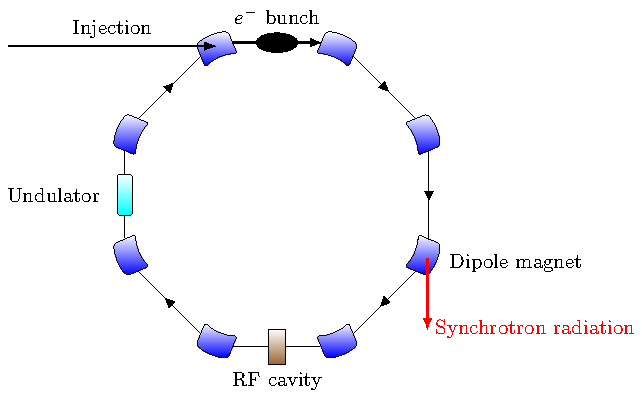
\includegraphics[width=0.7\textwidth]{chap/02-theory/img/synchrotron.pdf}
	\caption{Basic scheme of an electron storage ring (redrawn from \cite{roussel2014})}
	\label{fig:storageRing}
\end{figure}

The range of \gls{sr} reaches from hard X-rays down to the infrared region of the electromagnetic spectrum (see \autoref{fig:spectrum}). \Gls{sr} shows properties like high intensity, high collimation, polarisation and generation in pulses of well-defined time duration.
High intensity is necessary for better penetration of the matter under study.
It prevents unnecessary exposure of the matter outside the area of interest and  improves the image quality by producing less scatter radiation from these areas.
Well defined duration of the pulses allows to observe chemical reactions on short time scales.
Due to this properties, synchrotrons are used for microscopy, spectroscopy, and time-resolved experiments in such fields like condensed matter physics, biology, material science and many more.

\begin{figure}[H]
	\centering
	\includegraphics[width = \textwidth, height = 0.5\textwidth]{chap/02-theory/img/spectrum.tikz}
	\caption{Electromagnetic spectrum} %todo of what?
	\label{fig:spectrum}
\end{figure}


\paragraph{Karlsruhe Research Accelerator}
At the synchrotron light source \gls{kara}, the possibility to utilize the synchrotron as a source of \gls{thz} is actively researched. 
The photonic time-stretch \gls{daq}, which has been developed in this thesis, should also be integrated into the beam diagnostics system at \gls{kara}. 
Therefore, a short overview of some parameters of this facility has been given below.

\gls{kara} is located at the \gls{kit} and is operated by the \gls{ibpt}.
The storage ring can be filled up with up to 184 electron bunches with a distance of \SI{2}{\nano\second} ($\eqdev$ \SI{500}{\mega\hertz}) between two adjacent bunches.
The main accelerator parameters are listed in \autoref{tab:kara}. 

\begin{table}[tbh]
	\caption{Some KARA parameters \cite{rota2018}}
	\label{tab:kara}
	\centering
	\begin{tabular}{ll}
		\toprule
		\textbf{Parameter}                  & \textbf{Value}                \\ \midrule
		Beam energy (max.)                  & \SI{2.5}{\giga \electronvolt} \\
		Circumference                       & \SI{110}{\meter}              \\
		Revolution Frequency (one electron) & \SI{2.7}{\mega \hertz}        \\
		        \multicolumn{2}{c}{\textbf{Minimum bunch spacing}}          \\
		\quad multi-bunch                   & \SI{2}{\nano \second}         \\
		\quad single-bunch                  & \SI{368}{\nano \second}       \\
		          \multicolumn{2}{c}{\textbf{Bunch length (rms)}}           \\
		\quad normal operation              & \SI{45}{\pico \second}        \\
		\quad short bunch                   & \SI{2}{\pico \second}         \\ \bottomrule
	\end{tabular}
\end{table}

One scientific focus at \gls{kara} lies in the study of so-called ``micro-bunching instabilities'' which are described in the following.

\subsubsection*{Micro-Bunching Instabilities}
Increasing demands in current and future accelerators applications call for higher brilliance of the emitted radiation. 
Brilliance denotes describes both the brightness and the angular spread of the beam. 
Higher brilliance allows to see more detail in the material under study.
The higher brilliance is achieved by shortening the electron bunches. 
As illustrated in \autoref{fig:csr}, this results in emission of \gls{csr}, the spectrum of which spans from \SI{100}{\GHz} up to THz.
Due to this \gls{csr} the bunches interact with their own radiation as shown in \autoref{fig:electronInteract}, which introduces complex longitudinal dynamics.
\begin{figure}[tbh]
	\centering
	\begin{subfigure}{0.4\textwidth}
		\centering
		\includegraphics[height=0.4\textwidth]{chap/02-theory/img/SRincoherent.tikz}  
		\caption{Incoherent SR}
		\label{fig:srincoherent}
	\end{subfigure}
	\hfill
	\begin{subfigure}{0.4\textwidth}
		\centering
		\includegraphics[height=0.4\textwidth]{chap/02-theory/img/SRcoherent.tikz}  
		\caption{Cohenrent SR}
		\label{fig:srcoherent}
	\end{subfigure}
	\begin{center}
		\begin{subfigure}{0.4\textwidth}
			\centering
			\includegraphics[width=1.2\textwidth]{chap/02-theory/img/SRlegend.tikz}  
			\label{fig:srlegend}
		\end{subfigure}
	\end{center}
	\caption[Incoherent and coherent SR]{Incoherent \gls{sr} and coherent \gls{sr} due to shorter electron bunch length \cite{rota2018}}
	\label{fig:csr}
\end{figure}


\begin{figure}[tbh]
	\centering
	\includegraphics[width = 0.8\textwidth]{chap/02-theory/img/electronInteraction.tikz}
	\caption{Electrons interact with their own radiation \cite{Bielawski2019}}
	\label{fig:electronInteract}
\end{figure}
These dynamics are the so called micro-bunching instabilities, the formation of micro-structures (in the sub-millimeter range) in the longitudinal density profile of the electron bunches.
These instabilities occur in bursts and are hard to control, as they depend on a number of system parameters.
This imposes on one side a huge limitation to the stable operation of the overall system at high current density/short bunch length mode.
On the other side, these instabilities themselves emit brilliant \gls{thz} radiation that could be potentially used in imaging applications.
Such applications however require a stable power of the radiation. 
Therefore, a control of these instability bursts could potentially make them a source of \gls{thz} radiation for user-applications. 
A thorough understanding and studying of these beam dynamics is therefore an important step towards providing an applicable \gls{thz} source. \cite{rota2018,brosi}
In order to make such investigations possible, appropriate beam diagnostic systems are required, which are capable of both capturing (ultra-)fast and long-term changes in the bunch profile.  

\subsection*{Control of Micro-Bunching Instabilities}
The \gls{ultrasync} project, funded by ANR-DFG\footnote{\gls{anr}, \gls{dfg}}, has an objective of ultrafast study and control of electron bunches in synchrotron light sources.

There is the question of control (i.e. suppression) of the bursts of \gls{thz} radiation occurring during the micro-bunching instability.
The goal is to obtain a high power and stable coherent emission. 
The current experimental setup uses a relatively simple feedback loop:
\begin{itemize}
	\item A bolometer/Schottky barrier diode detector which produces the input signal for the feedback loop.
	\item A low-cost \gls{fpga} (Red Pitaya) that controls the the accelerating voltage of the synchrotron based on the input
\end{itemize} %todo Red Pitaya?

However, there are limitations in the controllable bunch charge in the accelerator this feedback loop can handle, which is around \SI{10}{\milli \ampere}. 
Therefore, an open question is whether measuring each \gls{thz} pulse using the setup
\begin{itemize}
	\item Electro-Optical sampling and time-stretching
	\item Association with the new \gls{fpga}-based system, i.e. \gls{theresa} system
	\item Finding adequate feedback, programmed in the \gls{fpga}
\end{itemize}
would help in solving the problem and allow the control to succeed also at higher currents (goal: \SI{15}{\milli \ampere}) \cite{bielwaski}.

\subsection{Electro-Optic Techniques for Longitudinal Bunch Profile Diagnostics}
Methods for analyzing the longitudinal profile of electron bunches are based on a similar, if not the same, electro-optical concept as the time-stretch method. 
Two most prominent methods are briefly described for the sake of completeness.
\subsubsection*{Scanning-Type Electro-Optic Sampling}
The scanning-type\gls{eos} samples one point at the time of the \gls{thz} pulse, emitted e.g. from an electron bunch, at each acquisition, hence the naming of this method.

A short laser pulse (duration typically hundreds of femtoseconds) co-propagates with a \gls{thz} pulse from \gls{csr} (range of picoseconds) in an \gls{eo} crystal. 
Due to the Pockels effect the \gls{thz} pulse causes a time dependent birefringence in the crystal.
This modulates the polarization state of the laser pulse.

To sample the pulse, the delay between the laser and the \gls{thz} pulse is varied.
To detect the changing polarization, the polarization of the laser pulse is transformed into an intensity modulation. This is done by using polarizers, e.g. \glspl{qwp} and \gls{wp} (as shown in \autoref{fig:scan_eo}).
A general scheme of the system is shown in \autoref{fig:scan_eo}.
For this technique a stable emission of the \gls{thz} pulses is crucial, as they are not measured in one acquisition. \cite{roussel2014}
\begin{figure}[tbh]
	\centering
	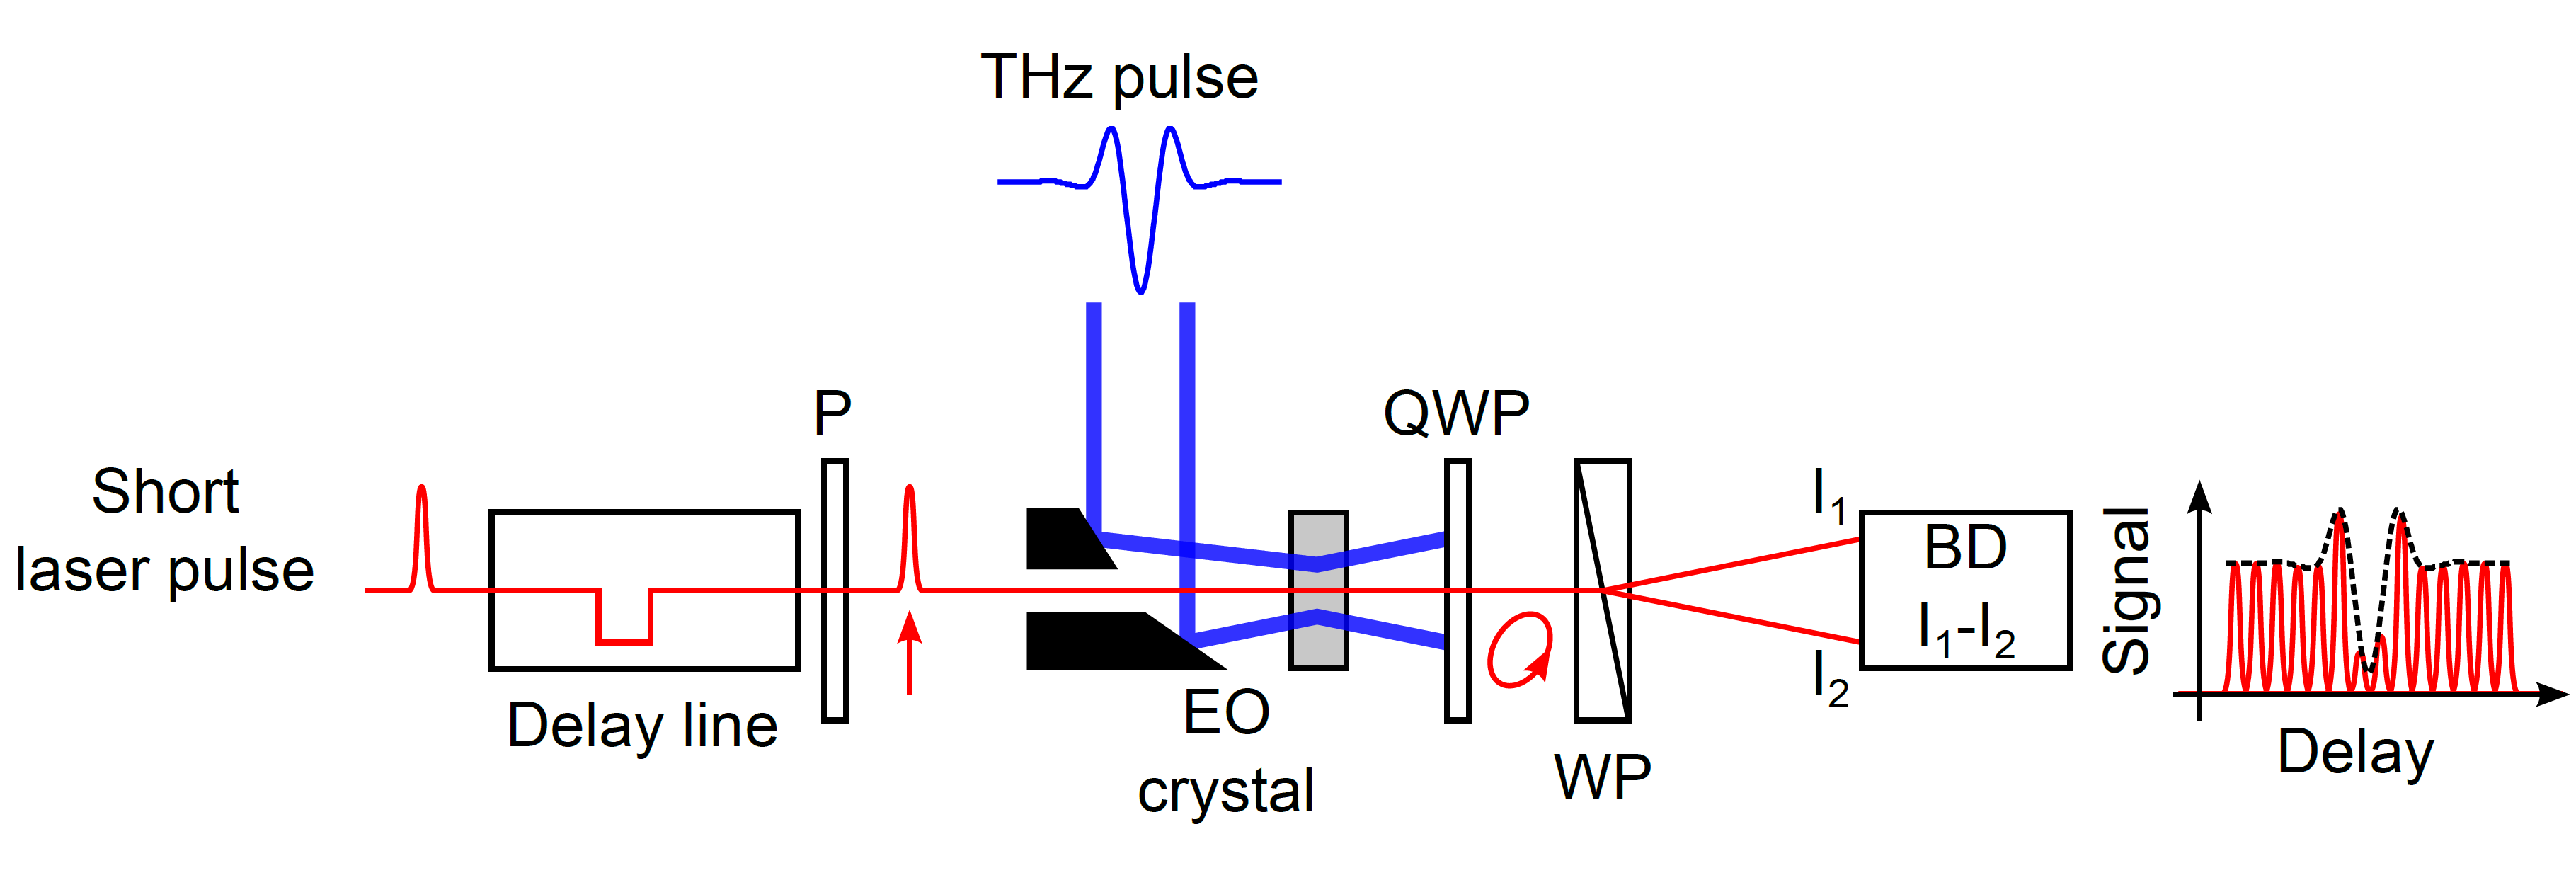
\includegraphics[width = \textwidth]{chap/02-theory/img/scanning_eo}
	\caption{Scheme of Scanning-Type Electro-Optical Sampling System \cite{roussel2014}}
	\label{fig:scan_eo}
\end{figure}


\subsubsection*{Spectrally Resolved Electro-Optic Detection}
In contrast to the \gls{eos}, single-acquisition is possible with the spectrally resolved \gls{eo} detection technique.
The short laser pulse is first stretched to a duration similar to the \gls{thz} pulse in a dispersive material, called stretcher.
In this way the pulse is chirped, meaning the instantaneous frequency of the pulse varies over time.
Together with the \gls{thz} pulse, the laser pulse propagates through an \gls{eo} crystal.
Again, the induced birefringence modulates the laser pulse, not only in time, but also in the spectral domain. %todo 'not only' -> due to the time/spectral duality or sth
The polarization state of the pulse is converted into an amplitude/intensity modulation.
This is done with a series of \gls{qwp}, \gls{hwp} and a polarizer (P) (as shown in \autoref{fig:spectral_eo}).
To retrieve the \gls{thz} pulse shape in time, the spectrum of the laser pulse is measured with a spectrometer. %todo what spectrometer (optical or electrical) or state model
A general scheme of the system is shown in \autoref{fig:spectral_eo}. \cite{roussel2014}

\begin{figure}[tbh]
	\centering
	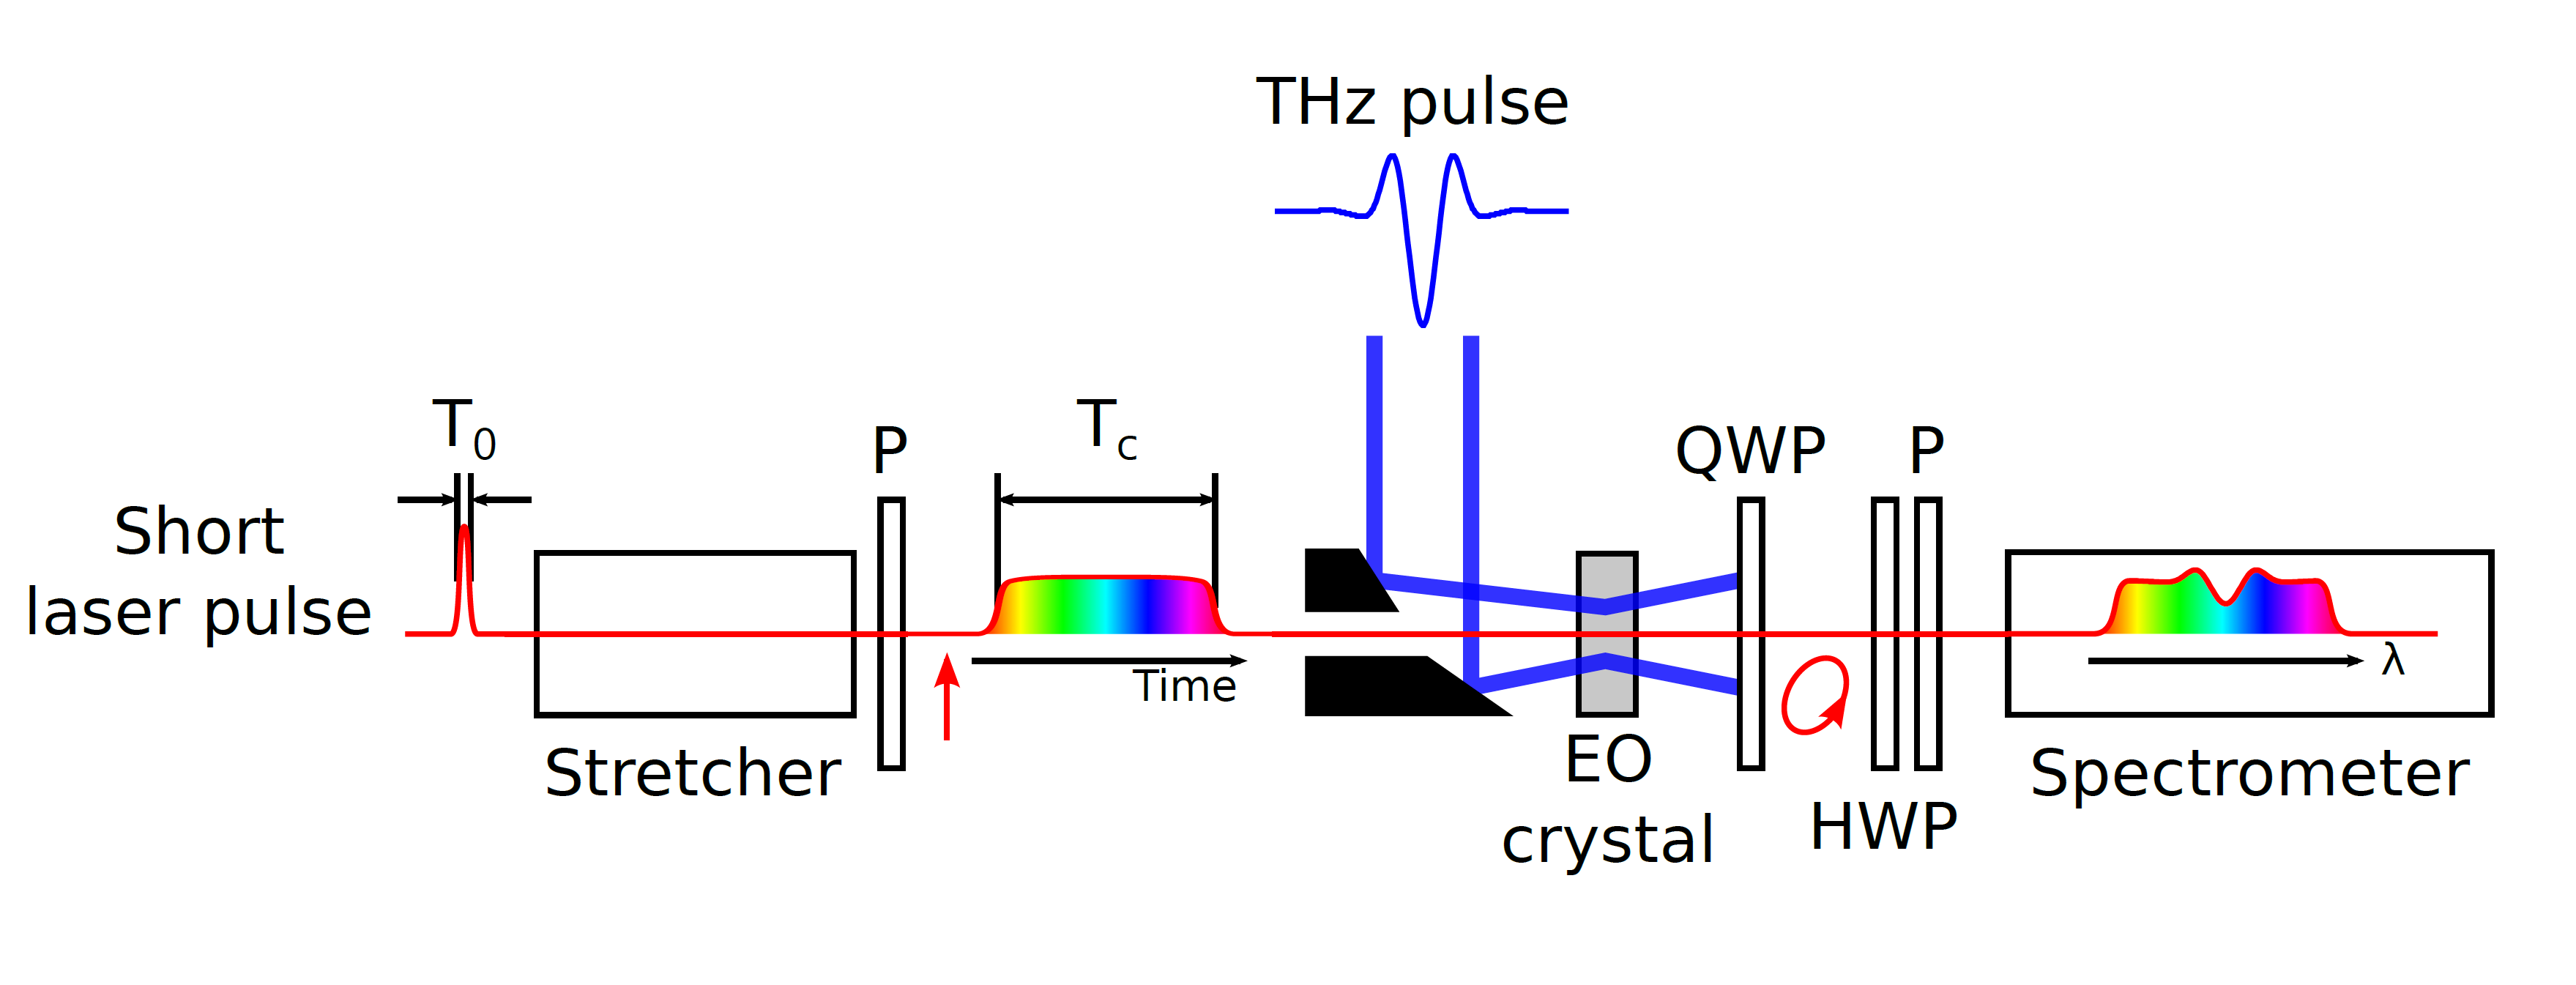
\includegraphics[width = \textwidth]{chap/02-theory/img/spectral_eo}
	\caption{Scheme of Spectrally Encoded Electro-Optical Detection System \cite{roussel2014}}
	\label{fig:spectral_eo}
\end{figure}

The temporal resolution of this method is limited due to the finite chirp rate
\begin{equation}
	\text{chirp rate} = \frac{\text{laser bandwidth}}{\text{laser pulse duration after stretcher}}.
\end{equation}

The minimal resolution $T_{\text{min}}$ depends on the bandwidth-limited pulse duration (before stretcher) $T_0$ and the duration of the chirped laser pulse $T_c$:
\begin{equation}
	T_{\text{min}} = \sqrt{T_0 T_c}
\end{equation}


\section{Photonic Time-Stretch Method}
The operating principle of the optical time-stretch technique can be described in three steps (see \autoref{fig:eo_ts}).

First, a short laser pulse (duration typically hundreds of femtoseconds) propagates in a dispersive medium, e.g. an optical fiber of length $L_1$ (see \autoref{fig:eo_ts}).
With the optical bandwidth of the laser pulse $\Delta \lambda$ and the dispersion parameter $D_1$ of the fiber, this results in a chirped laser pulse of the duration
\begin{equation}
	T_1 = \Delta \lambda D_1 L_1.
\end{equation}
The next step is the time-to-wavelength-mapping, where a temporal intensity modulation is imprinted on the chirped pulse.
This happens when the laser pulse co-propagates with another pulse, e.g. a \gls{thz} pulse from \gls{csr} (duration in the range of picoseconds), in an \gls{eo} crystal. 
Due to the Pockels effect the \gls{thz} pulse causes a time-dependent birefringence in the crystal. 
The Pockels effect describes the phenomenon of occurring and change of existing birefringence in an electric field, which is linearly proportional to the electric field strength. \cite{pockels} 

After that, the modulated chirped pulse propagates through another dispersive medium, a fiber of the length $L_2$.
In this way, the temporal modulation of the pulse is further stretched to the duration $T_2$, which is long enough for detection with photodetectors and the digitizing with \Glspl{adc}. \cite{roussel2014} 

The factor $M$, by which the pulse is slowed down, is calculated as
\begin{equation}\label{eq:ts}
	M = 1 + \frac{L_2}{L_1}.
\end{equation}
As example, assume the length of the dispersive media as $L_1 = \SI{10}{\meter}$ and $L_2 = \SI{2}{\kilo \meter}$ and an input signal with the duration $t_\text{sig} = T_1 = \SI{1}{\pico \second}$. 
With \autoref{eq:ts} the stretching factor for this set-up is $M \approx 200$. The input pulse is stretched to $T_2 = M \cdot T_1 = 200 \cdot \SI{1}{\pico \second} = \SI{200}{\pico \second} = \SI{0.2}{\nano \second}$.
This corresponds to a frequency of $\SI{5}{\GHz}$ which is much easier to handle e.g. for an oscilloscope.

\begin{figure}[tbh]
	\centering
	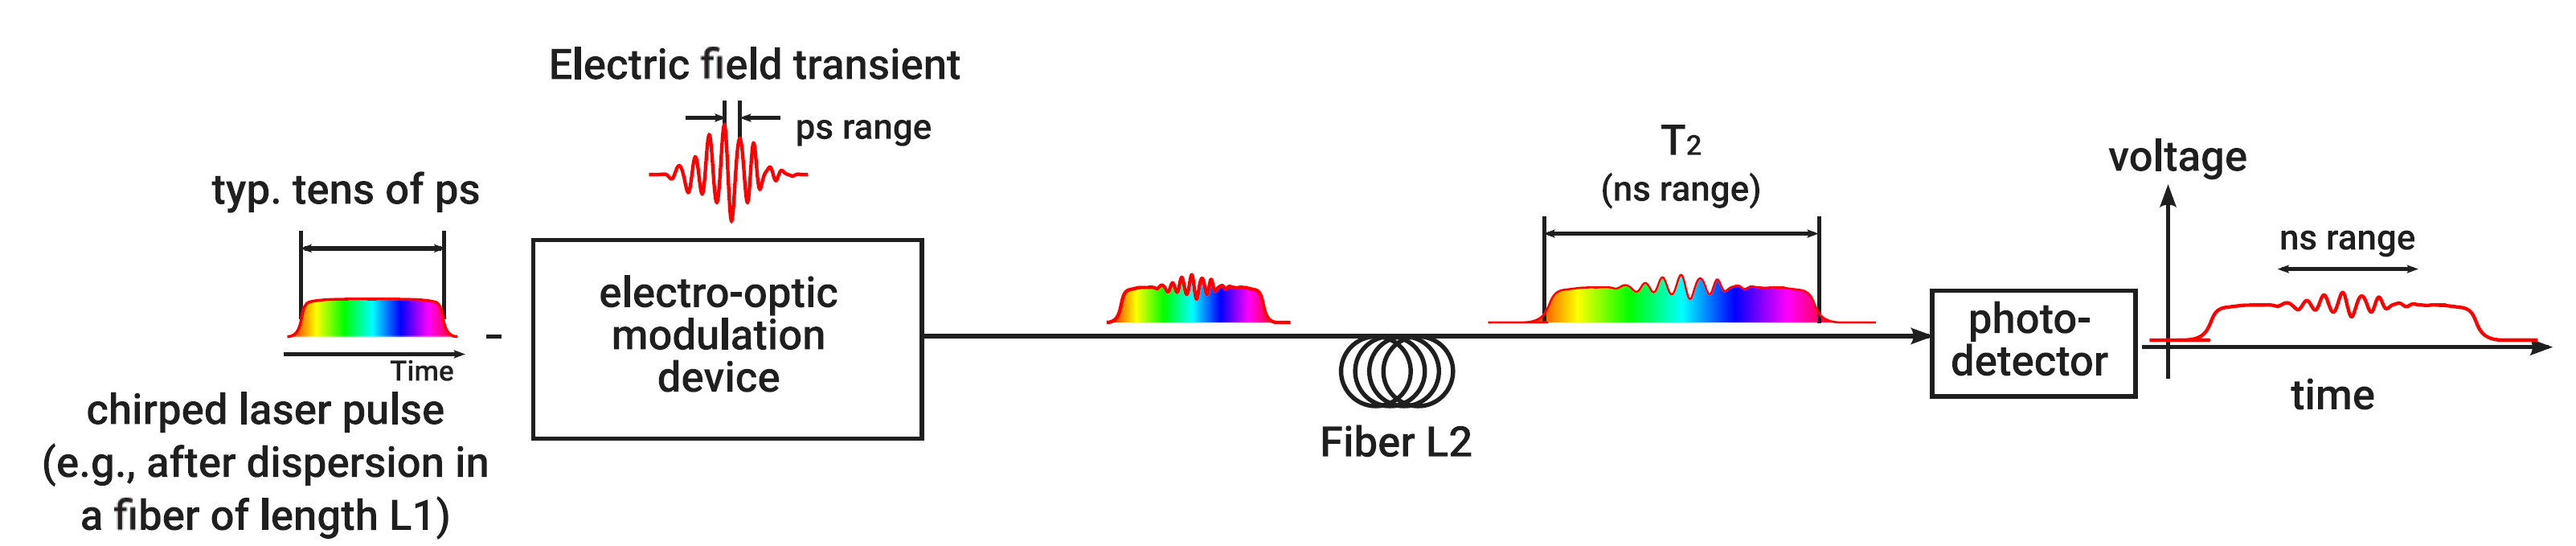
\includegraphics[width = \textwidth]{chap/02-theory/img/time_stretch.png}
	\caption{Working principle of the electro-optical time-stretch technique \cite{roussel2014}}
	\label{fig:eo_ts}
\end{figure}

\paragraph{Photodetector}
In order to convert the time-stretched optical signal into an electrical value a photodetector, e.g. a photodiode, is needed.
A basic diode photodetector is a photo-diode operated in reverse bias, meaning the $p$-side is connected to the negative terminal and the $n$-side to the positive terminal of the power supply. %todo typically with some resistor to set the op and not fry the diode
This enlarges the depletion region (see \autoref{fig:pn_junc}) of the $p/n$-junction as the depletion region contains only a very small amount of free charge carriers. 
Irradiating diode with photons of sufficient energy generates electron-hole pairs due to the photoelectric effect. %todo check my changes
If the electron-hole pairs are produced in the depleted region of the $p/n$-junction, they are separated by the electric field applied across it, before they can recombine. 
This creates a so called photo-current which can be measured. \cite{photodiode} %todo with a trans impedance amplifier maybe for the 'voltages' in the next section

\begin{figure}[tbh]
	\centering
	\includegraphics[]{chap/02-theory/img/pn.tikz}
	\caption{pn-junction with depleted region \cite{pn-junc}}
	\label{fig:pn_junc}
\end{figure}


\section{Analog-To-Digital Converter}
\Glspl{adc} are used to translate analog signals, like voltages, into the digital representation of these signals.
This \textit{digitized} version can then be stored and processed by information processing, computing, data transmission and control systems. 
This translation, also called ``conversion'', can be seen as encoding a continuous-time analog input $V_\text{in}$ (voltage) into a series of discrete, $N$-bit words. %todo $V_\text{in}(t)$ ?
This process is also called \textit{sampling}. 
With the full-scale voltage of the $V_{\text{FS}}$, the individual output bits $b_k$ and the quantization error $\epsilon$, the \gls{adc} should satisfy the relation
\begin{equation} \label{eq:adc_sample}
	V_{\text{in}} = V_{\text{FS}} \sum_{k = 0}^{N-1} \frac{b_k}{2^{k+1}} + \epsilon.
\end{equation}
%todo what is full scale voltage, lsb, v_q, \epsi?
This can also be rewritten in terms of the \gls{lsb} or quantum level $V_Q$
\begin{equation}
	1 \text{LSB} = \frac{V_\text{FS}}{2^N} = V_Q.
\end{equation}
With \autoref{eq:adc_sample} this leads to 
\begin{equation}
	V_\text{in} = V_Q \sum_{k = 0}^{N-1} b_k 2^{k}  + \epsilon.
\end{equation}

\autoref{fig:idealADC} shows the ideal transfer function of a 3-bit \gls{adc}. 
Each digital $N$-bit word corresponds to a range of input voltage values (\textit{code width}), which is centered around a \textit{code center}.
The input voltage is resolved to the code of the nearest code center.
\begin{figure}[H]
	\centering
	\includegraphics[width = 0.7\textwidth]{chap/02-theory/img/ideal_adc}
	\caption[Transfer function of ideal, 3-bit ADC]{Transfer function of an ideal, 3-bit \gls{adc} (redrawn from \cite{Lundberg})}
	\label{fig:idealADC}
\end{figure}


\paragraph{Sample-And-Hold-Amplifier}
\Glspl{adc} need a certain amount of time to sample the input signal.
If the level of the analog signal changes by more than one \gls{lsb} during this period, this can result in large errors in the output signal.
Therefore so called \gls{sha} are used in front of the \gls{adc} to hold the input level constant for the needed amount of time.

A general block diagram of a \gls{sha} is shown in \autoref{fig:tha}. %todo correct figure? THA vs SHA?
It consists of an input and output buffer, a switch controlled by the sampling clock and a capacitor.
The analog input is buffered in an input buffer which leads to a switch that is controlled by a sampling clock.
During the sample mode, i.e. during the negative sampling clock cycle, the switch is open.
At the transition from negative to positive clock cycle, the switch closes, connecting the input signal with the capacitor which is charged in this way.

The \gls{adc} sampling time needs to be timed in such way, that the whole duration of an analog-to-digital conversion falls into the hold period of the \gls{sha} and does not exceed into the sample period. 
\autoref{fig:sha_timing} shows a qualitative example for proper sample timing. 
As conclusion, the upper frequency limitation is not determined by the \gls{adc} itself, but rather by the aperture jitter, bandwidth, distortion, etc. of the \gls{sha}. \cite{walt}

\begin{figure} [H]
	\centering
	\tikzexternaldisable
	\includegraphics[width=\linewidth]{chap/02-theory/img/sha_timing.tikz}  
	\tikzexternalenable
	\caption[SHA timing example]{Example for appropriate sampling timing when using Sample-And-Hold-Amplifier. The sample points of the \gls{adc} should be inside the period, where the \gls{sha} holds the input value.}
	\label{fig:sha_timing}
\end{figure}
\paragraph{Track-And-Hold Amplifier}
Apart from the \glspl{sha} there also exists the so called \gls{tha}.
Though the names are often used interchangeably, there exists one fundamental difference between a \gls{sha} and a \gls{tha}.
Strictly speaking, the output of a \gls{sha} is not defined during the sample period. 
Only when switching to the hold mode, the output is assigned to a defined value: the voltage level at the input in that moment.
Contrary to that, the \gls{tha} acts as a unity gain amplifier during the sample period, meaning the output is just a replication of the input. 
The \gls{tha} ``tracks'' the input signal (see also \autoref{fig:sha_timing}).
Therefore, instead of speaking of a ``sample'' period, the term used here is the ``track'' period.
When switching to hold mode, the instantaneous input level is held over the course of the hold period.
This principle allows to improve the sampling rate, as the settling time of an \gls{tha} is in general smaller than one of a \gls{sha}.
Settling time denotes the amount of time needed for the output voltage to be at a stable level, after the transition from track/sample to hold mode.
This process is quicker, when the output voltage is already in the range of the sampled input at the moment, instead of when the hold capacitor first has to be charged to the input voltage. \cite{Reeder2017}


\begin{figure}[tbh]
	\centering
	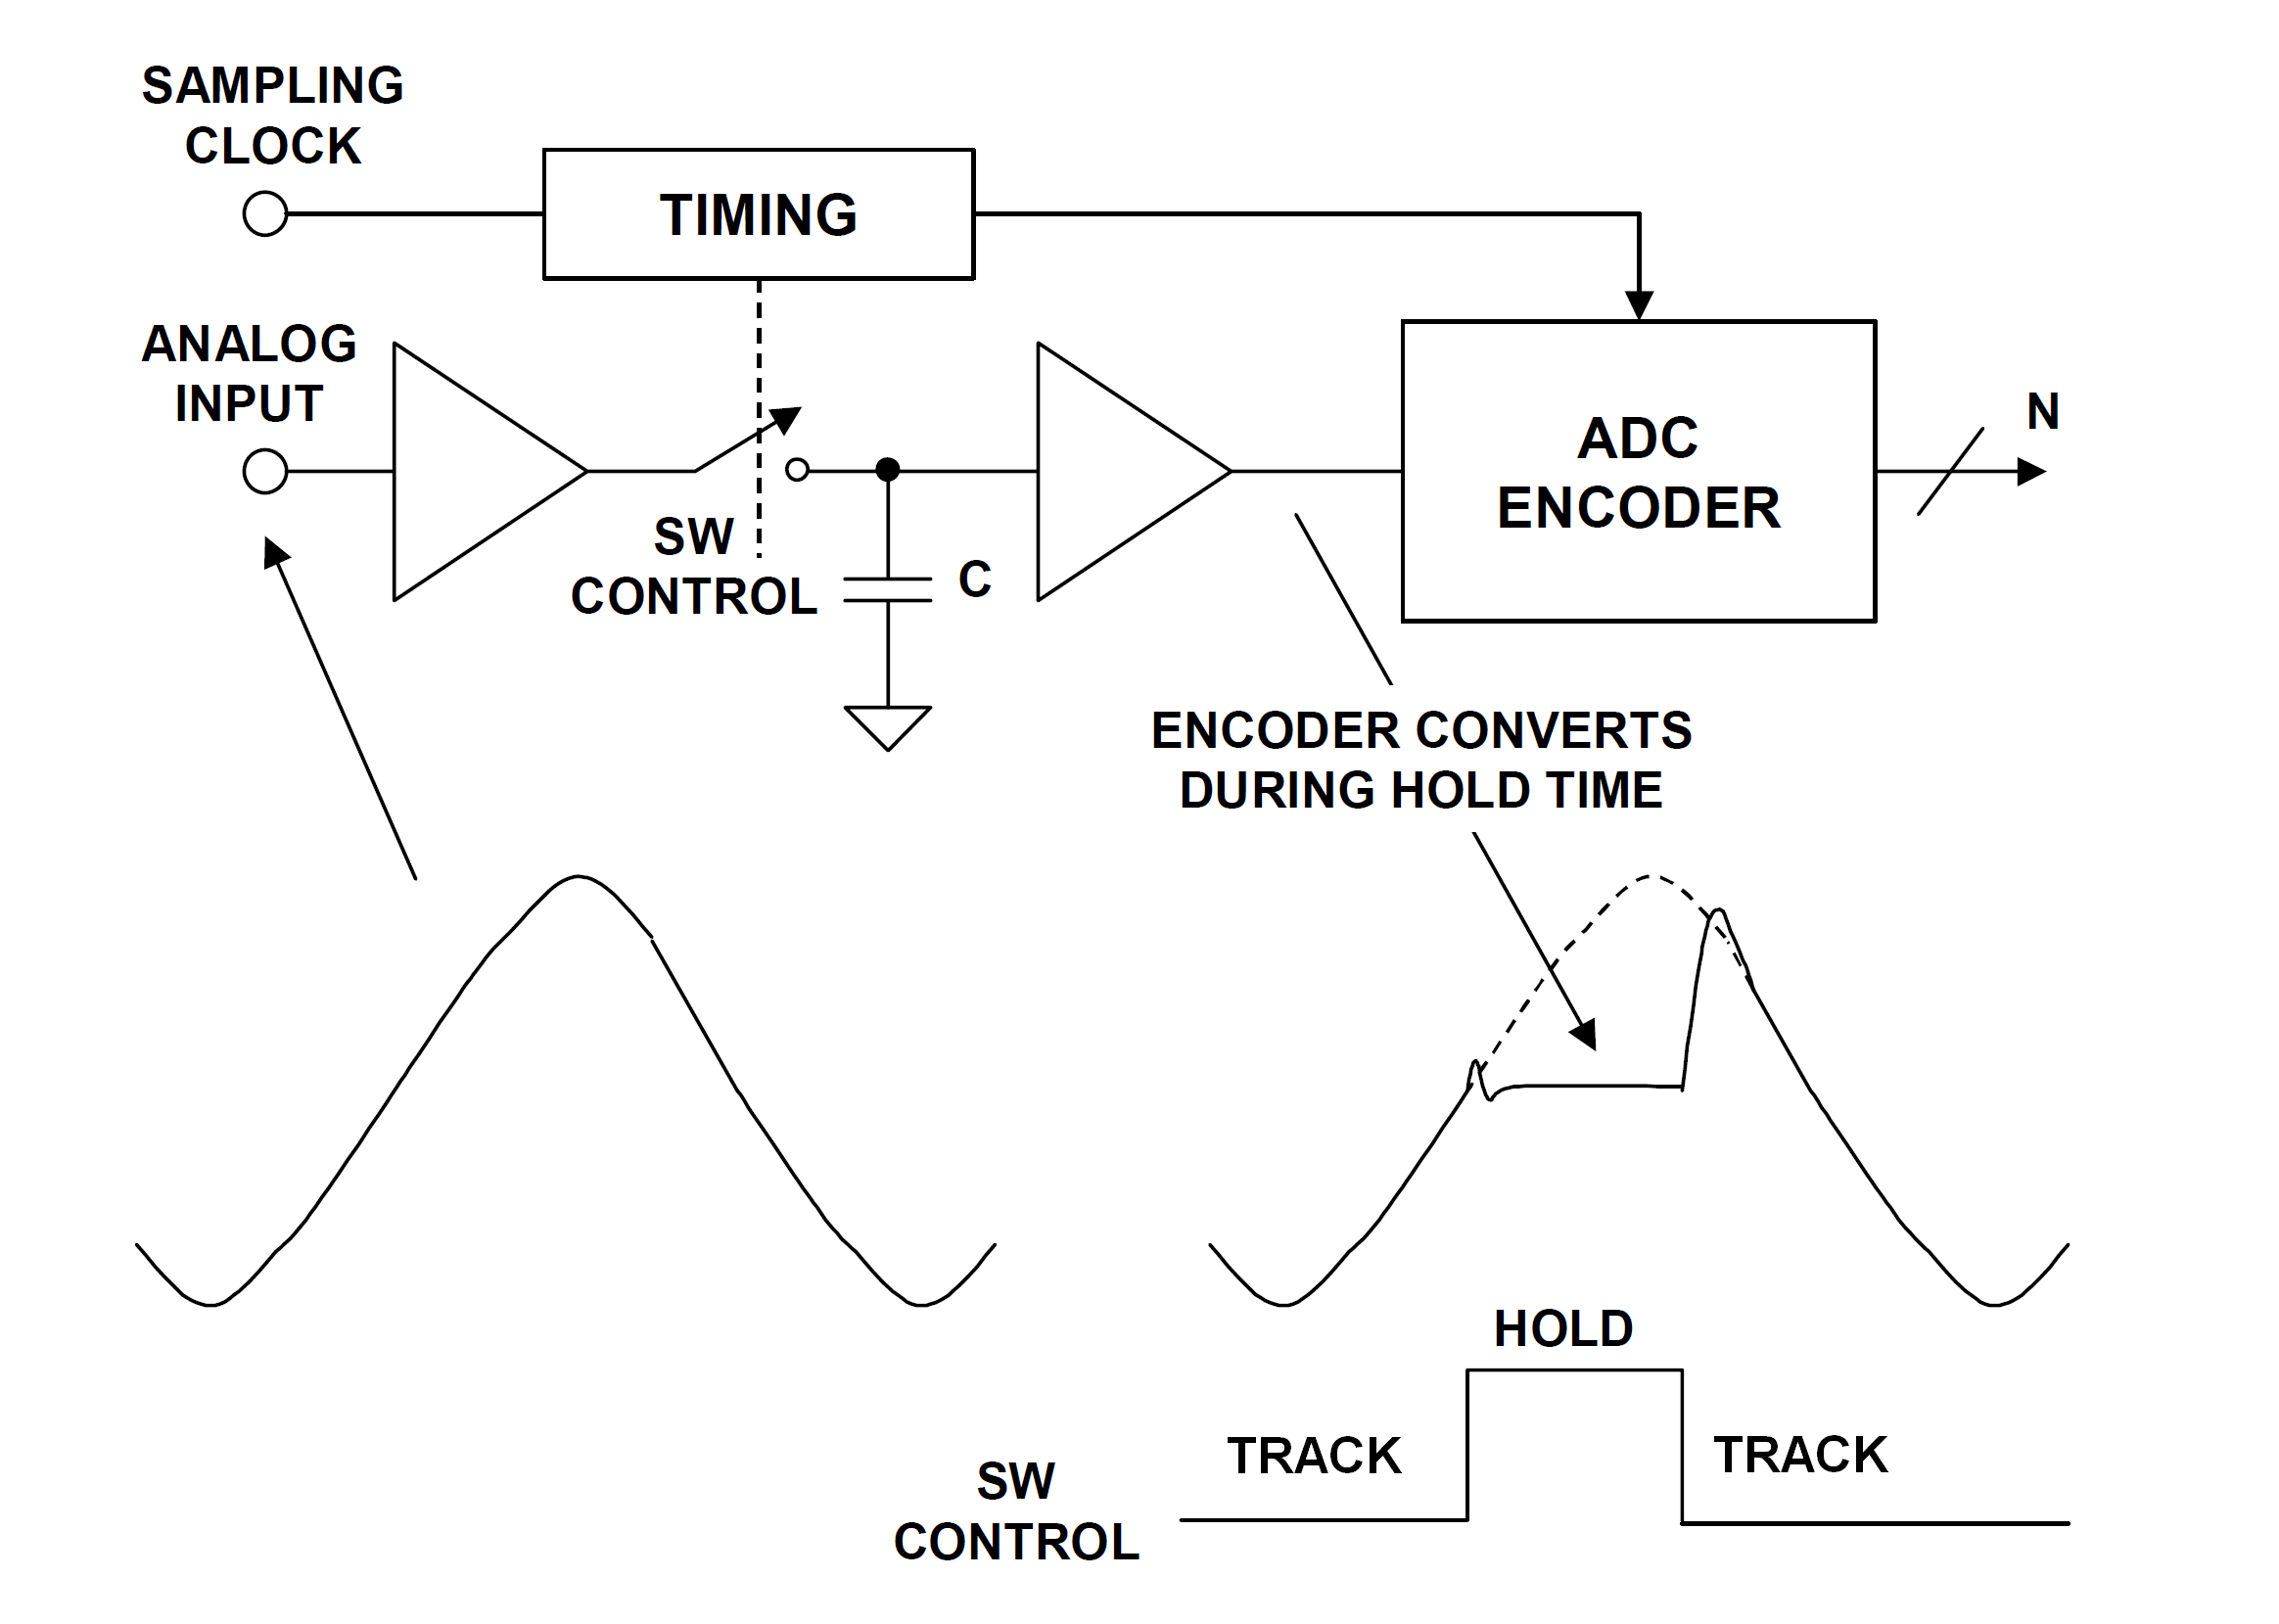
\includegraphics[width = \textwidth]{chap/02-theory/img/tha}
	\caption{Track-And-Hold-Amplifier schematic and principle \cite{walt}}
	\label{fig:tha}
\end{figure}

\subsection{Characteristics of Analog-To-Digital-Converters}\label{ssec:adc_charac}
For an ideal converter, the number of bits and the sampling rate would be sufficient to fully characterize its performance.
Real \glspl{adc} however differ from the ideal behavior by introducing static and dynamic imperfections.
Different applications have different requirements, which leads to a number of specifications.
These can be divided into the categories according to \cite{Lundberg}:
\begin{itemize}[noitemsep]
	\item Quantization Noise
	\item Static parameters
	\item Frequency-domain dynamic parameters
	\item Time-domain dynamic parameters
\end{itemize} %todo which of those are static, which dynamic?
This section provides an overview of these figures of merit.
Which of them are needed to specify the necessary performance of the \gls{adc} has to be chosen for each application accordingly.

\subsubsection{Quantization Noise}\label{par:quant_noise}
Even an ideal $N$-bit converter has errors resulting from the quantization process which behave like noise. %todo maybe can be modelled as noise, or shows as noise instead of behave
The reason is that each $N$-bit word represents a certain range of analog input values, which is 1 \gls{lsb} wide and centered around a code center (see \autoref{fig:idealADC}). \cite{Lundberg}
The input voltage is assigned to the word of the nearest code center.
This means that there will always be a difference between the corresponding voltage of the respective digital code $x_q(t)$ and the actual analog input voltage $x(t)$.
This difference is called the \textit{quantization error}. For an equidistant quantization, the quantization error for a code width $q$ is (see \cite{puente2015})
\begin{equation}
	\left| e_q(t) \right| = \left| x(t) - x_q(t) \right| \leq \frac{q}{2}.
\end{equation}
A setup in order to measure this quantization error is shown in \autoref{fig:qe_m}. 
\begin{figure}[tbh]
	\centering
	\includegraphics[width = \textwidth]{chap/02-theory/img/quant_err_meas.tikz}
	\caption[Measurement setup for quantization error]{Setup for measuring the quantization error of an (ideal) \gls{adc} with input signal $x(t)$}
	\label{fig:qe_m}
\end{figure}

The output of the \gls{adc}, the $N$-bit code corresponding to the voltage level of the input signal $x(t)$, is fed to a \gls{dac}, which converts this code into a corresponding voltage level $x_q(t)$. 
The difference between $x(t)$ and $x_q(t)$ is the quantization error $e_q(t)$.

In order to analyze the quantization noise and the resulting theoretical (maximum) \gls{snr} of the ideal \gls{adc}, assume a ramp with the slope $s$ as an input signal. 
Then, the quantization error $e_q(t)$ can be approximated with a sawtooth signal in the time domain (see \cite{walt}): 
\begin{equation}\label{eq:qe_saw}
	e_q(t) = st, \quad -\frac{q}{2s} < t < \frac{q}{2s} 
\end{equation}
The function in \autoref{eq:qe_saw} is plotted in \autoref{fig:eq}.
\begin{figure}[tbh]
	\centering
	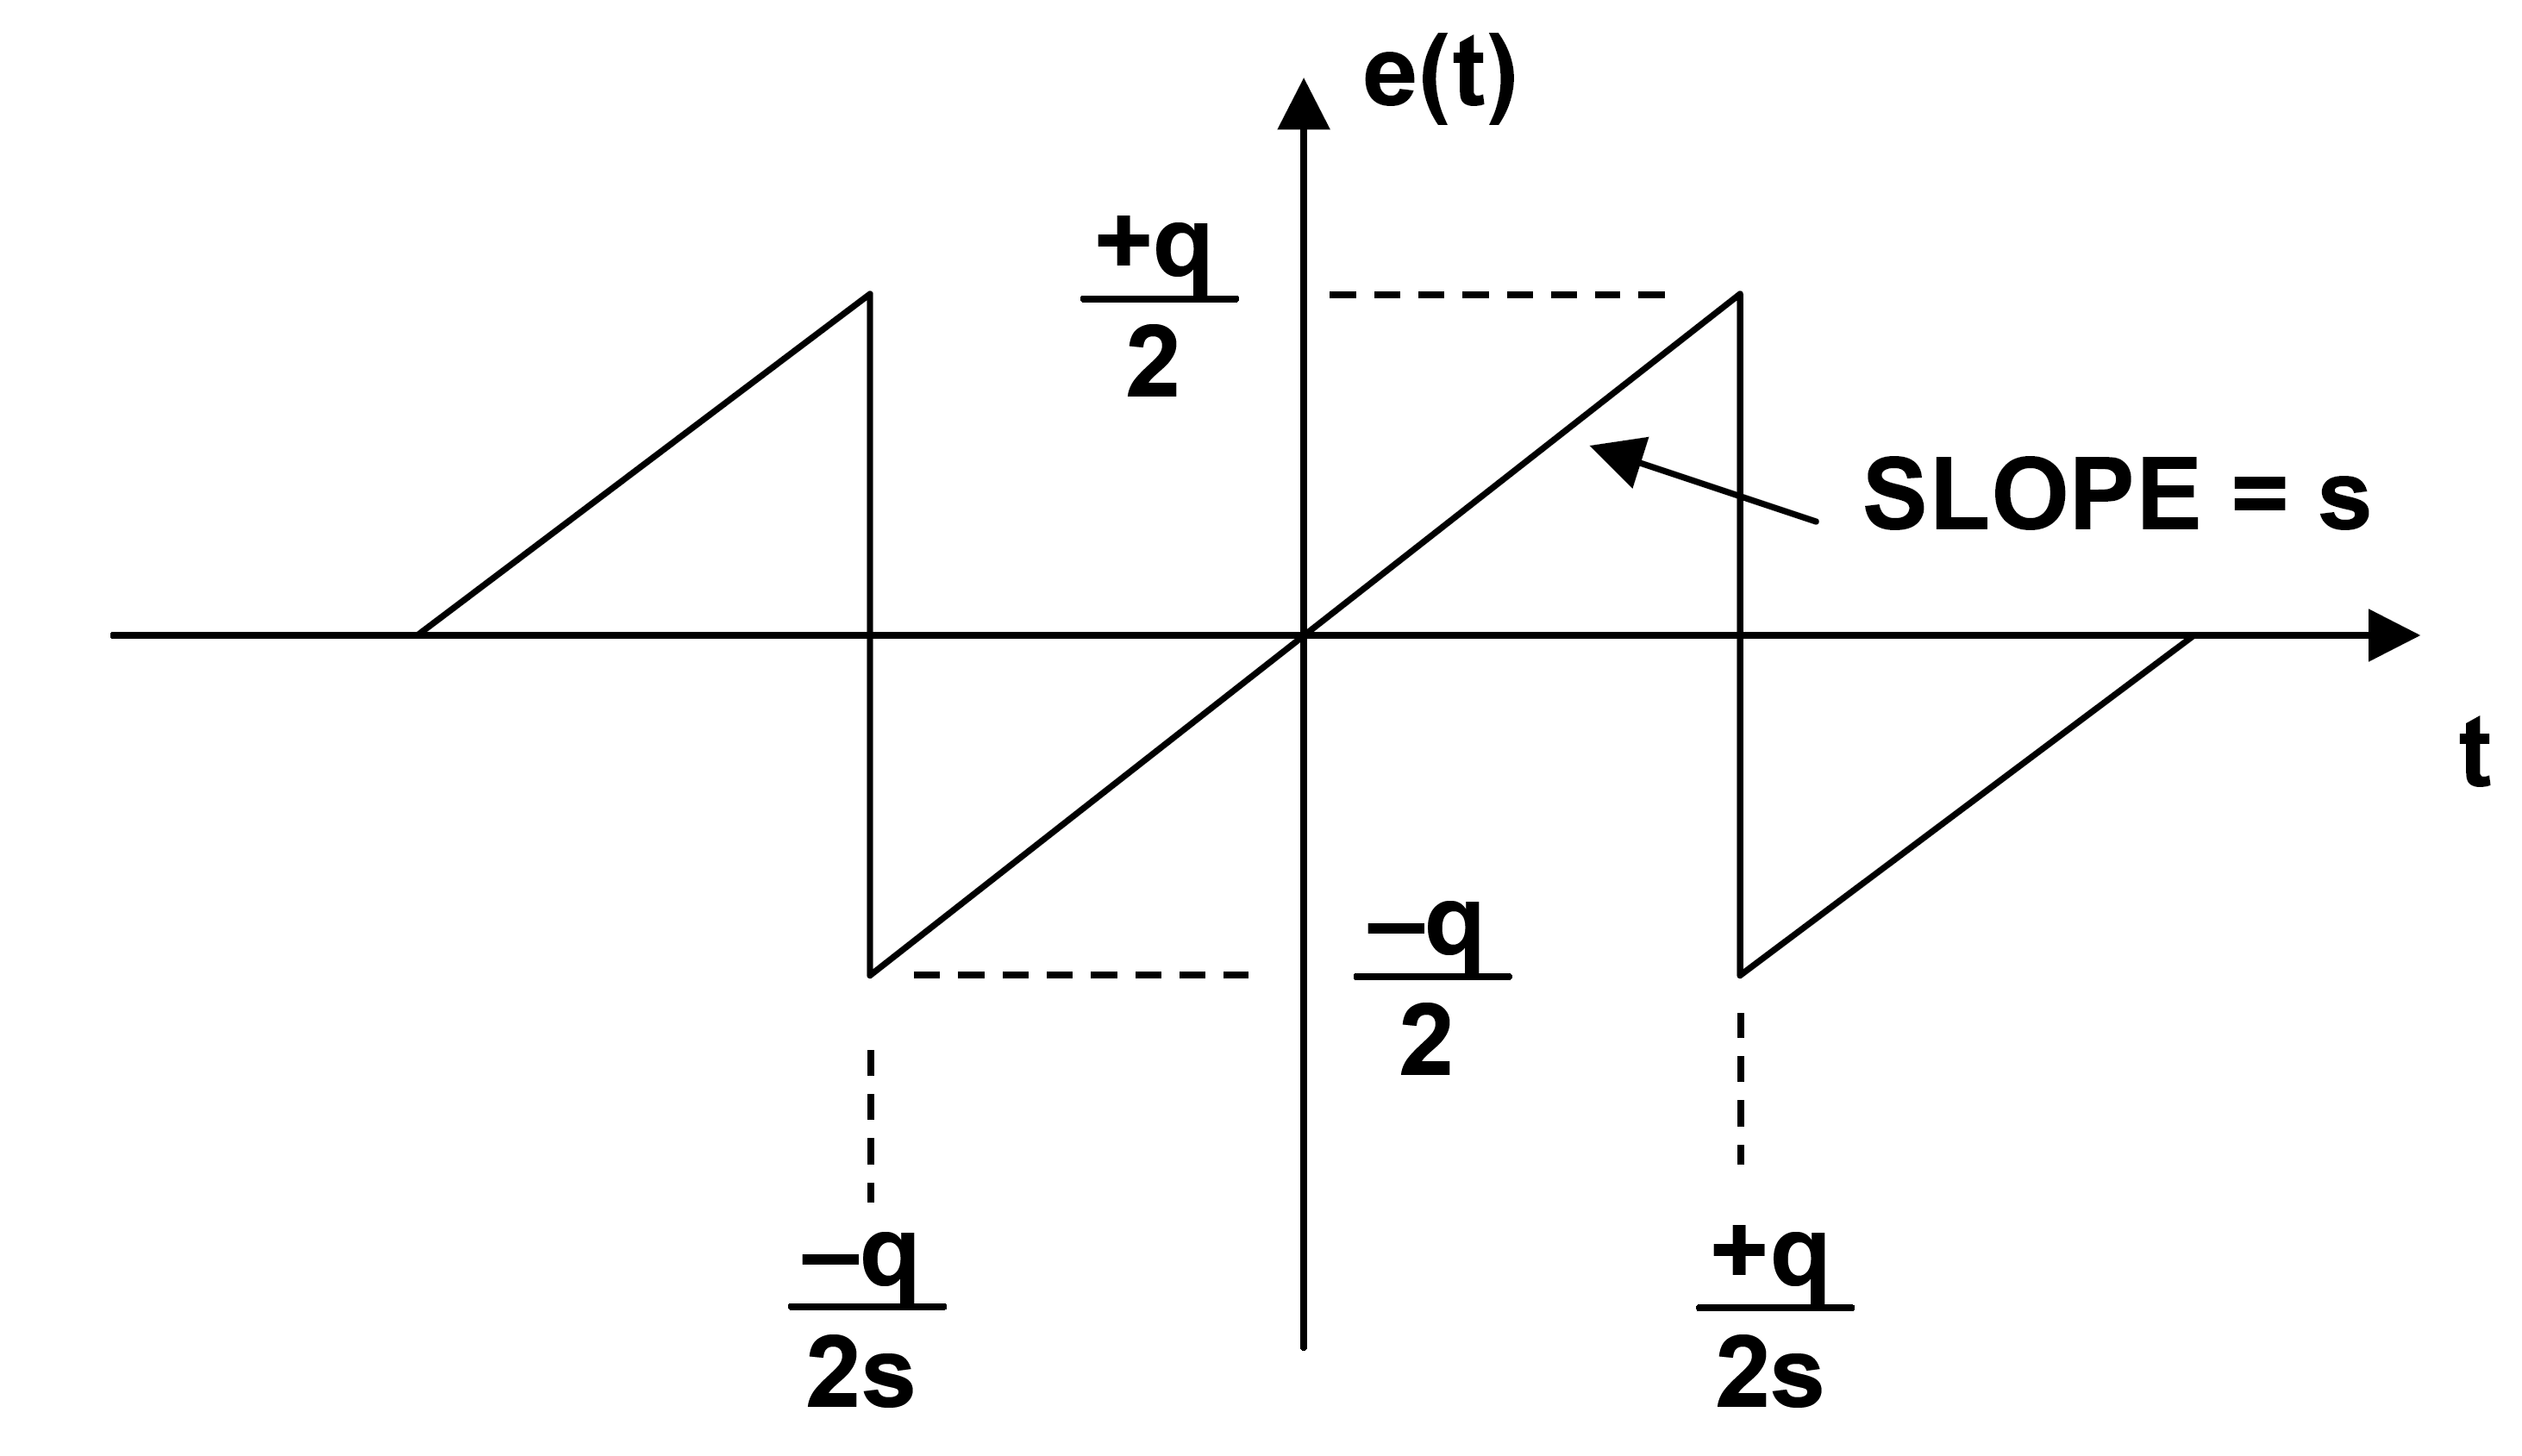
\includegraphics[width = 0.7\textwidth]{chap/02-theory/img/quantization_error.tikz}
	\caption{Quantization noise as function of time (redrawn from \cite{walt})}
	\label{fig:eq}
\end{figure}

The power of this quantization noise can be calculated as the mean-square $e_{\text{rms}}^2$ of $e(t)$ (see \cite{walt}):
\begin{equation}
	P_{QN} = e_{\text{rms}}^{2} = \overline{e^{2}(t)} = \frac{s}{q}\int_{-q/2s}^{+q/2s} (st)^{2} dt = \frac{s^3}{q} \left[ \frac{t^3}{3}\right]_{-\frac{q}{2s}}^{+\frac{q}{2s}} = \frac{q^2}{12}
\end{equation}

In order to calculate the maximal \gls{snr} of an ideal converter, a full-scale input sine wave is applied to the input:
\begin{equation}
	u(t) = u_s \sin(2\pi f t) = \frac{2^{N}q}{2}\sin(2\pi f t)  = 2^{N-1}q \sin(2\pi f t)
\end{equation}
With the effective value of the signal amplitude
\begin{equation}
	u_{\text{eff}} = \frac{u_s}{\sqrt{2}} = \frac{2^{N-1}q}{\sqrt{2}}
\end{equation}
the \gls{snr} can be calculated as 
\begin{equation}
	\text{SNR} = \frac{P_{\text{signal}}}{P_{\text{noise}}} = \frac{u_{\text{eff}}^{2}}{e_{\text{rms}}^{2}} = \frac{2^{2N-2}q^2/2}{q^2/12} = 2^{2N} \cdot 1.5.
\end{equation}
In decibel, the \gls{snr} is calculated as (see \cite{puente2015, walt}):
\begin{equation}\label{eq:idealSNR}
	\text{SNR}|_{\text{dB}} = 10\log\left(2^{2N}\cdot 1.5\right) = 6.02 N + 1.76
\end{equation}




\subsubsection{Static parameters}
\textit{Static parameters} are specifications, which can be measured at low speed/DC. 
\paragraph{Accuracy}
\textit{Accuracy} is the total error with which an \gls{adc} can convert a known voltage, which includes the effects of (see \cite{Lundberg}):
\begin{itemize}[noitemsep]
	\item Quantization error
	\item Gain error
	\item Offset error
	\item Non-linearities
\end{itemize}

\paragraph{Resolution}
\textit{Resolution} is the number of bits $N$ of the \gls{adc}.
Depending from the resolution are the size of the \gls{lsb}, which in its turn determines the dynamic range, code widths and quantization error.
\paragraph{Dynamic Range}
The \textit{dynamic range} represents the ratio between smallest possible output (\gls{lsb} voltage) and the largest possible output (full-scale voltage).
It can be calculated as
\begin{equation}
	20 \log 2^{N} \approx 6N.
\end{equation}

\paragraph{Offset and Gain Error}
The \textit{offset error} is defined as the deviation of the actual \gls{adc} transfer function from the ideal \gls{adc} transfer function in the point of zero. It is measured in \gls{lsb}. 
 
\textit{Gain Error} defines the deviation of the slope of the line going through the zero and full-scale point of the transfer function. %todo state eq for 'transfer function' otherwise 'line', 'zero' and 'full-scale point' undefined here
\autoref{fig:offsetErr} visualizes the effects of both offset and gain error. 
\begin{figure}[tbh]
	\centering
	\includegraphics[width = 0.8\textwidth]{chap/02-theory/img/adc_offset_gain.tikz}
	\caption[Effects of Offset and Fain error in ADC]{Offset and Gain Error in the \gls{adc} characteristic transfer function. The offset error is indicated with the red arrow. The gain error expresses itself via different slope of the real \gls{adc} (dotted) compared to the ideal \gls{adc} (dashed)}
	\label{fig:offsetErr}
\end{figure}

These errors can easily be corrected by calibration. 
In order to measure the offset and gain error, two different voltage levels $V_1$ and $V_2$ are applied at the \gls{adc} input. 
This results in corresponding bit codes $b_1$ and $b_2$.
The slope $s$ of the transfer function can then be calculated by
\begin{equation}
	s = \frac{b_2 - b_1}{V_2 - V_1}.
\end{equation}
From this, the gain error can be determined.
In order to obtain the offset error $b$, the linear equation
\begin{equation}
	b = b_1 - s\cdot V_1
\end{equation}
is solved.


%todo where is this full-scale point here in the fig?

\paragraph{Integral and Differential Non-Linearity Distortion} 
\gls{inl} is the distance of the code centers on the actual \gls{adc} transfer function from the ideal line (dashed line in \autoref{fig:nld}). %todo which transfer function?
It results from the integral non-linearities of the front-end, \gls{sha} and also the \gls{adc} itself \cite{walt, Lundberg}. 

\gls{dnl} is the deviation in actual code width from the ideal width of 1 \gls{lsb}. This non-linearity stems exclusively from the encoding process in the \gls{adc} \cite{Lundberg,walt} . 

The effect of these errors is shown in \autoref{fig:nld}.
\begin{figure}[tbh]
	\centering
	\includegraphics[width = 0.8\textwidth]{chap/02-theory/img/nonlinear.tikz}
	\caption[ADC Nonlinearities]{Transfer function of a real \gls{adc} showing \gls{dnl} and \gls{inl}.\cite{Lundberg}}
	\label{fig:nld}
\end{figure}

These non-linearities could be measured with a histogram test.
A voltage ramp is applied at the input and the number of occurrences of each \gls{adc} output code, $n$(code), is measured.
With the ramp slope $s$ am ideal \gls{adc} with the sampling frequency $f_s$ would give
\begin{equation}
	n(\text{code}) = \frac{\text{LSB}}{s} \cdot f_s = n_\text{avg},
\end{equation}
which ideally would be constant for the whole input range (except for the first and last code).
For a real \gls{adc} this is not the case and the \gls{dnl} and \gls{inl} are calculated as (see \cite{inlDnl})
\begin{align}
	\text{DNL(code)} &= \frac{n(\text{code})-n_\text{avg}}{n_\text{avg}}\\
	\text{INL(code)} &= \sum_{i = 0}^{\text{code}} \text{DNL}(i).
\end{align}


\subsubsection{Frequency-Domain Dynamic Parameters}
Any real \gls{adc} is subject to noise distortion. 
\textit{Noise} denotes any unwanted random signal, which interferes with the measuring of the desired signal. 
Examples are quantization noise or random fluctuations due to thermal noise. 
\textit{Distortion} is the term for alteration of the shape of the original signal. 
As an example, distortion of the amplitude might result due to not equal amplification of the parts of a signal. \cite{nd}

In an \gls{adc} (with built-in \gls{sha}) there are a couple of sources, which introduce noise and distortion:
\begin{itemize}
	\item \textbf{Input Stage:} Wideband noise, non-linearity and bandwidth limitation
	\item \textbf{\gls{sha}:} Non-linearity, aperture jitter(see paragraph about Time-Domain Dynamic Performances) and bandwidth limitation %todo use label/autoref here
	\item \textbf{\gls{adc}:} Quantization noise, non-linearity
\end{itemize}

For quantification of noise and distortion, frequency-domain metrics are used. 
Therefore the figures of merit described in the following paragraphs are also called frequency-domain dynamic parameters. 
These parameters are measured with the help of the \gls{fft} meaning any modern oscilloscope can be used to quickly assess the frequency-domain dynamic performance for a given input at the \gls{adc}.
As some parameters, such as \gls{sfdr}, are only defined for one carrier input frequency, several measurements at different input frequencies need to be made in order to fully characterize the \gls{adc}.

In the following paragraphs, an overview of the metrics for quantification of the noise and distortion of an \gls{adc} is given. 


\paragraph{Signal-to-Noise Ratio}
The \gls{snr} is defined as the ratio of the input signal power to the power of the noise signal. 
It is expressed in dB and can be calculated using the \gls{rms} value of the signal and noise amplitudes (see \cite{xilinx_adc}):
\begin{align}
	\text{SNR} &= \frac{\text{Power}_\text{Signal}}{\text{Power}_\text{Noise}}\\
	&= \left( \frac{\text{Amplitude}_\text{Signal,rms}}{\text{Amplitude}_\text{Noise,rms}} \right)^2\\
	&= 20 \log \left( \frac{V_\text{in,rms}}{V_\text{Q,rms}}\right) 
\end{align}
Usually, the \gls{snr} degrades at higher frequencies due to sampling jitter. \cite{xilinx_adc}

\paragraph{Signal-to-Noise-and-Distortion Ratio}
\gls{sinad} (also called SNDR or S/N+D) denotes the ratio between the \gls{rms} of the signal amplitude to the mean value of the Root-Sum-Square (RSS) of all other spectral components, including harmonics, but excluding \gls{dc} (\SI{0}{\hertz}). 
\gls{sinad} is a good indication over the general dynamic performance of the \gls{adc}, as it includes all contributions from noise and distortion.
The higher the \gls{sinad} the stronger the input power is differentiated from noise and spurious components. 

\gls{sinad} can be calculated from the average power of the input signal $P_\text{signal}$, noise $P_\text{noise}$ and $P_\text{distortion}$:
\begin{equation}
	\text{SINAD} = 10 \log \left( \frac{P_\text{signal}}{P_\text{noise} + P_\text{Distortion}} \right)
\end{equation}
It is commonly expressed in dB, \gls{dbc} or \gls{dbfs}.

\paragraph{Effective-Number-Of-Bits}
The \gls{enob} expresses the \gls{sinad} in terms of bits. It can be calculated as (see \cite{walt2009})
\begin{equation}
	\text{ENOB} = \frac{\text{SINAD}-\SI{1.76}{\decibel}}{\SI{6.02}{\decibel}/\text{bit}}. \quad 
\end{equation}
This is derived from solving the equation of the ``ideal \gls{snr}'' (\autoref{eq:idealSNR}) for the number of bits $N$ and substituting \gls{snr} with \gls{sinad}.
This however means, that this parameter assumes a full-scale input signal. Expressing the \gls{enob} for a smaller signal amplitude requires measuring the \gls{sinad} at this level and a correction factor. \cite{walt}

\paragraph{Spurious-Free Dynamic Range}
\gls{sfdr} indicates the dynamic range of the converter, which can be used, before there is interference or distortion from spurious components with the fundamental signal. \cite{Lundberg} 
The \gls{sfdr} is calculated as the \gls{rms} value of the fundamental signal to the \gls{rms} value of the worst spurious signal, i.e. the highest spur in the spectrum.
It is measured over the whole Nyquist bandwidth from \gls{dc} to $f_s/2$, with $f_s$ being the \gls{adc} sampling rate. The spur may or may not be a harmonic of the fundamental signal. \cite{walt2009, Lundberg}

The \gls{sfdr} is an important characteristic in the sense, that it indicates the smallest signal which can still be distinguished from a strong interfering signal. \cite{walt2009} 

The \gls{sfdr} in dBc can be calculated as (see \cite{xilinx_adc})%todo what is dbc?
\begin{equation}
	\text{SFDR}_\text{dBc} = 20 \log \left( \frac{\text{Fundamental Amplitude (RMS)}}{\text{Largest Spur Amplitude (RMS)}} \right).
\end{equation}


\autoref{fig:sfdr} illustrates the \gls{sfdr} in terms of \gls{dbfs} and \gls{dbc}.

\begin{figure}[tbh]
	\centering
	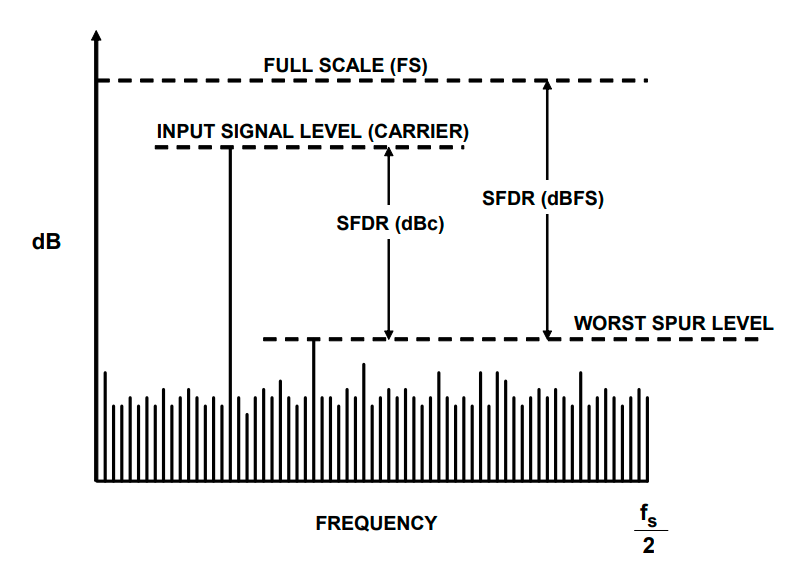
\includegraphics[width = \textwidth]{chap/02-theory/img/sfdr.tikz}
	\caption[SFDR definition]{Visualization of the \gls{sfdr}. It can be indicated either with reference to the carrier frequency in ``dBc'' or with reference to the Full-Scale Input in ``dBFS''. \cite{walt2009}}
	\label{fig:sfdr}
\end{figure}
\paragraph{Total Harmonic Distortion}
The \textit{Total Harmonic Distortion} describes the ratio of the \gls{rms} sum of the first five harmonic components (or aliased versions of them) to the \gls{rms} of the considered fundamental signal. \cite{Lundberg}

\paragraph{Effective Resolution Bandwidth}
\textit{Effective Resolution Bandwidth} denotes the frequency of the input signal, at which the \gls{sinad} has fallen by \SI{3}{\decibel} ($\eqdev$ 0.5 bit in terms of \gls{enob}) compared to the \gls{sinad} at lower frequency range. \cite{Lundberg}

\paragraph{Analog Input Bandwidth}
\textit{Analog Input Bandwidth} is the analog input frequency at which the power of the fundamental is reduced by 3dB with respect to the low-frequency value. \cite{Lundberg}
It is not to be confused with the maximal analog input frequency which the \gls{adc} is able to sample.

\paragraph{Full-Linear Bandwidth}
The \textit{Full-Linear Bandwidth} is defined as the frequency at which the slew-rate of the \gls{sha} starts to distort the input signal by a specified value. \cite{Lundberg} 
The slew-rate (SR) is defined as the rate of how much the voltage $v$ changes over time $t$:
\begin{equation}
	\text{SR} = \frac{\text{d}v}{\text{d}t}
\end{equation}
A slew-rate of \SI{1}{\volt \per \micro \second} for example means, that the output of the amplifier can not change more than \SI{1}{\volt} over the course of \SI{1}{\micro \second}.\cite{2021Slew} 

\paragraph{Time-Domain Dynamic Parameters}
Time-Domain Dynamic parameters describe the deviation of the converter's behavior from the ideal one in time domain. 

\paragraph{Aperture Delay}
\textit{Aperture Delay} (or \textit{aperture time}) is defined as delay between the triggering of the converter (e.g. rising edge of the sampling clock) and the actual conversion of the input voltage into the digitized value. \cite{Lundberg}

\paragraph{Aperture Jitter}
\textit{Aperture jitter} describes the sample-to-sample variation in aperture delay. Jitter can cause significant error in the voltage and decreases the overall \gls{snr} of a converter.
Especially for high-speed \glspl{adc} jitter poses a limit in performance.

Assuming a full-scale sinus-wave $V_{\text{in}}$ as input signal with 
\begin{equation}
	V_{\text{in}} = V_{\text{FS}} \sin(\omega t)
\end{equation}
the maximal slope of this signal is then
\begin{equation}
	\frac{\text{d}V_{\text{in}}}{\text{d}t}\Bigr|_{\text{max}} = \omega V_{\text{FS}}
\end{equation}
Aperture jitter $\Delta t_{\text{rms}}$ occurring during the sampling of this maximal slope produces the \gls{rms} voltage error 
\begin{equation}
	\Delta V_{\text{rms}} = \omega  V_{\text{FS}} \Delta t_{\text{rms}} = 2 \pi f  V_{\text{FS}} \Delta t_{\text{rms}}.
\end{equation}
As variations in aperture time occur randomly, these errors behave like a random noise source. This way, a \gls{sjnr} can be defined as
\begin{equation}
	\text{SJNR} = 20 \log \left( \frac{V_{\text{FS}}}{\Delta V_{\text{rms}}} \right) = 20 \log \left( \frac{1}{2 \pi f  V_{\text{FS}}} \right)
\end{equation}

The voltage error due to jitter and the \gls{sjnr} for different aperture jitter values are shown in \autoref{fig:ap_jit}.

\begin{figure}[tbh]
	\centering
	\begin{subfigure}{0.48\textwidth}
		\centering
		\includegraphics[width=\textwidth]{chap/02-theory/img/jitterTimeDomain.tikz}  
		\caption{Effect of aperture jitter}
		\label{fig:jitter}
	\end{subfigure}
	\hfill
	\begin{subfigure}{0.48\textwidth}
		\centering
		\includegraphics[height=\textwidth]{chap/02-theory/img/SJNRjitter.tikz}  
		\caption{SJNR for different aperture jitter values}
		\label{fig:sjnr}
	\end{subfigure}
	\caption[Aperture jitter and SJNR]{Effects of aperture jitter and SJNR. Left: In time domain, Right: SJNR for different aperture jitter \cite{Lundberg}}
	\label{fig:ap_jit}
\end{figure}

\paragraph{Transient Response}
The \textit{transient response} denotes the settling time of an \gls{adc} until full accuracy ($\pm$ 1/2 \gls{lsb}).


\subsubsection{Sampling Theory}
%todo cite http://fab.cba.mit.edu/classes/S62.12/docs/Shannon_noise.pdf and https://ieeexplore.ieee.org/document/5055024
An \gls{adc} samples an analog signal with a sample frequency $f_s$.
This frequency has to be chosen in such way, that the original signal can be fully reconstructed.
The \textit{Nyquist criteria} states, that in order to accurately reconstruct continuous signal limited to the bandwidth $B$
\begin{equation}
	y (t) \, \fourier  Y(f) \quad \text{with} \quad Y(f)=0\vert_{f>B/2}
\end{equation} %todo one bobble at fourier missing?
it has to be sampled with a frequency $f_s$ respecting
\begin{equation} \label{eq:nyquist}
	f_s > B \quad \text{or} \quad f_s > 2 f_a,
\end{equation}
with $f_a$ being the highest frequency contained in the signal. \cite{walt,puente2015}
The range from \SI{0}{\Hz} to $\nicefrac{f_s}{2}$ is also called \textit{Nyquist-Zone} (or ``1st Nyquist zone'', see \autoref{fig:alias_f}).
%todo why not relate f_a to B?

Violation of this rule leads to \textit{aliasing}.
The effects of aliasing are shown in \autoref{fig:aliasing}.

When a harmonic wave of the frequency $f_a$ is sampled with the frequency $f_s$, this leads to periodic repetition of the signal spectrum in frequency domain in intervals of $f_s$, or ``images'' (see dashed, red frequency components in \autoref{fig:alias_f}). 
If \autoref{eq:nyquist} is respected, i.e. $f_a$ lies inside the Nyquist bandwidth, there is no overlap with the images created by the sampling process.

Now assuming a signal frequency $f_a \approx f_s$, the sampling process leads to an image falling inside the Nyquist bandwidth.
The reconstructed signal then lies at the frequency of this image which is much lower than the original frequency.
The result of this \textit{undersampling} is shown in \autoref{fig:alias_t}.


%todo explain aliasing


\begin{figure}[tbh]
	\centering
	\begin{subfigure}{\textwidth}
		\centering
		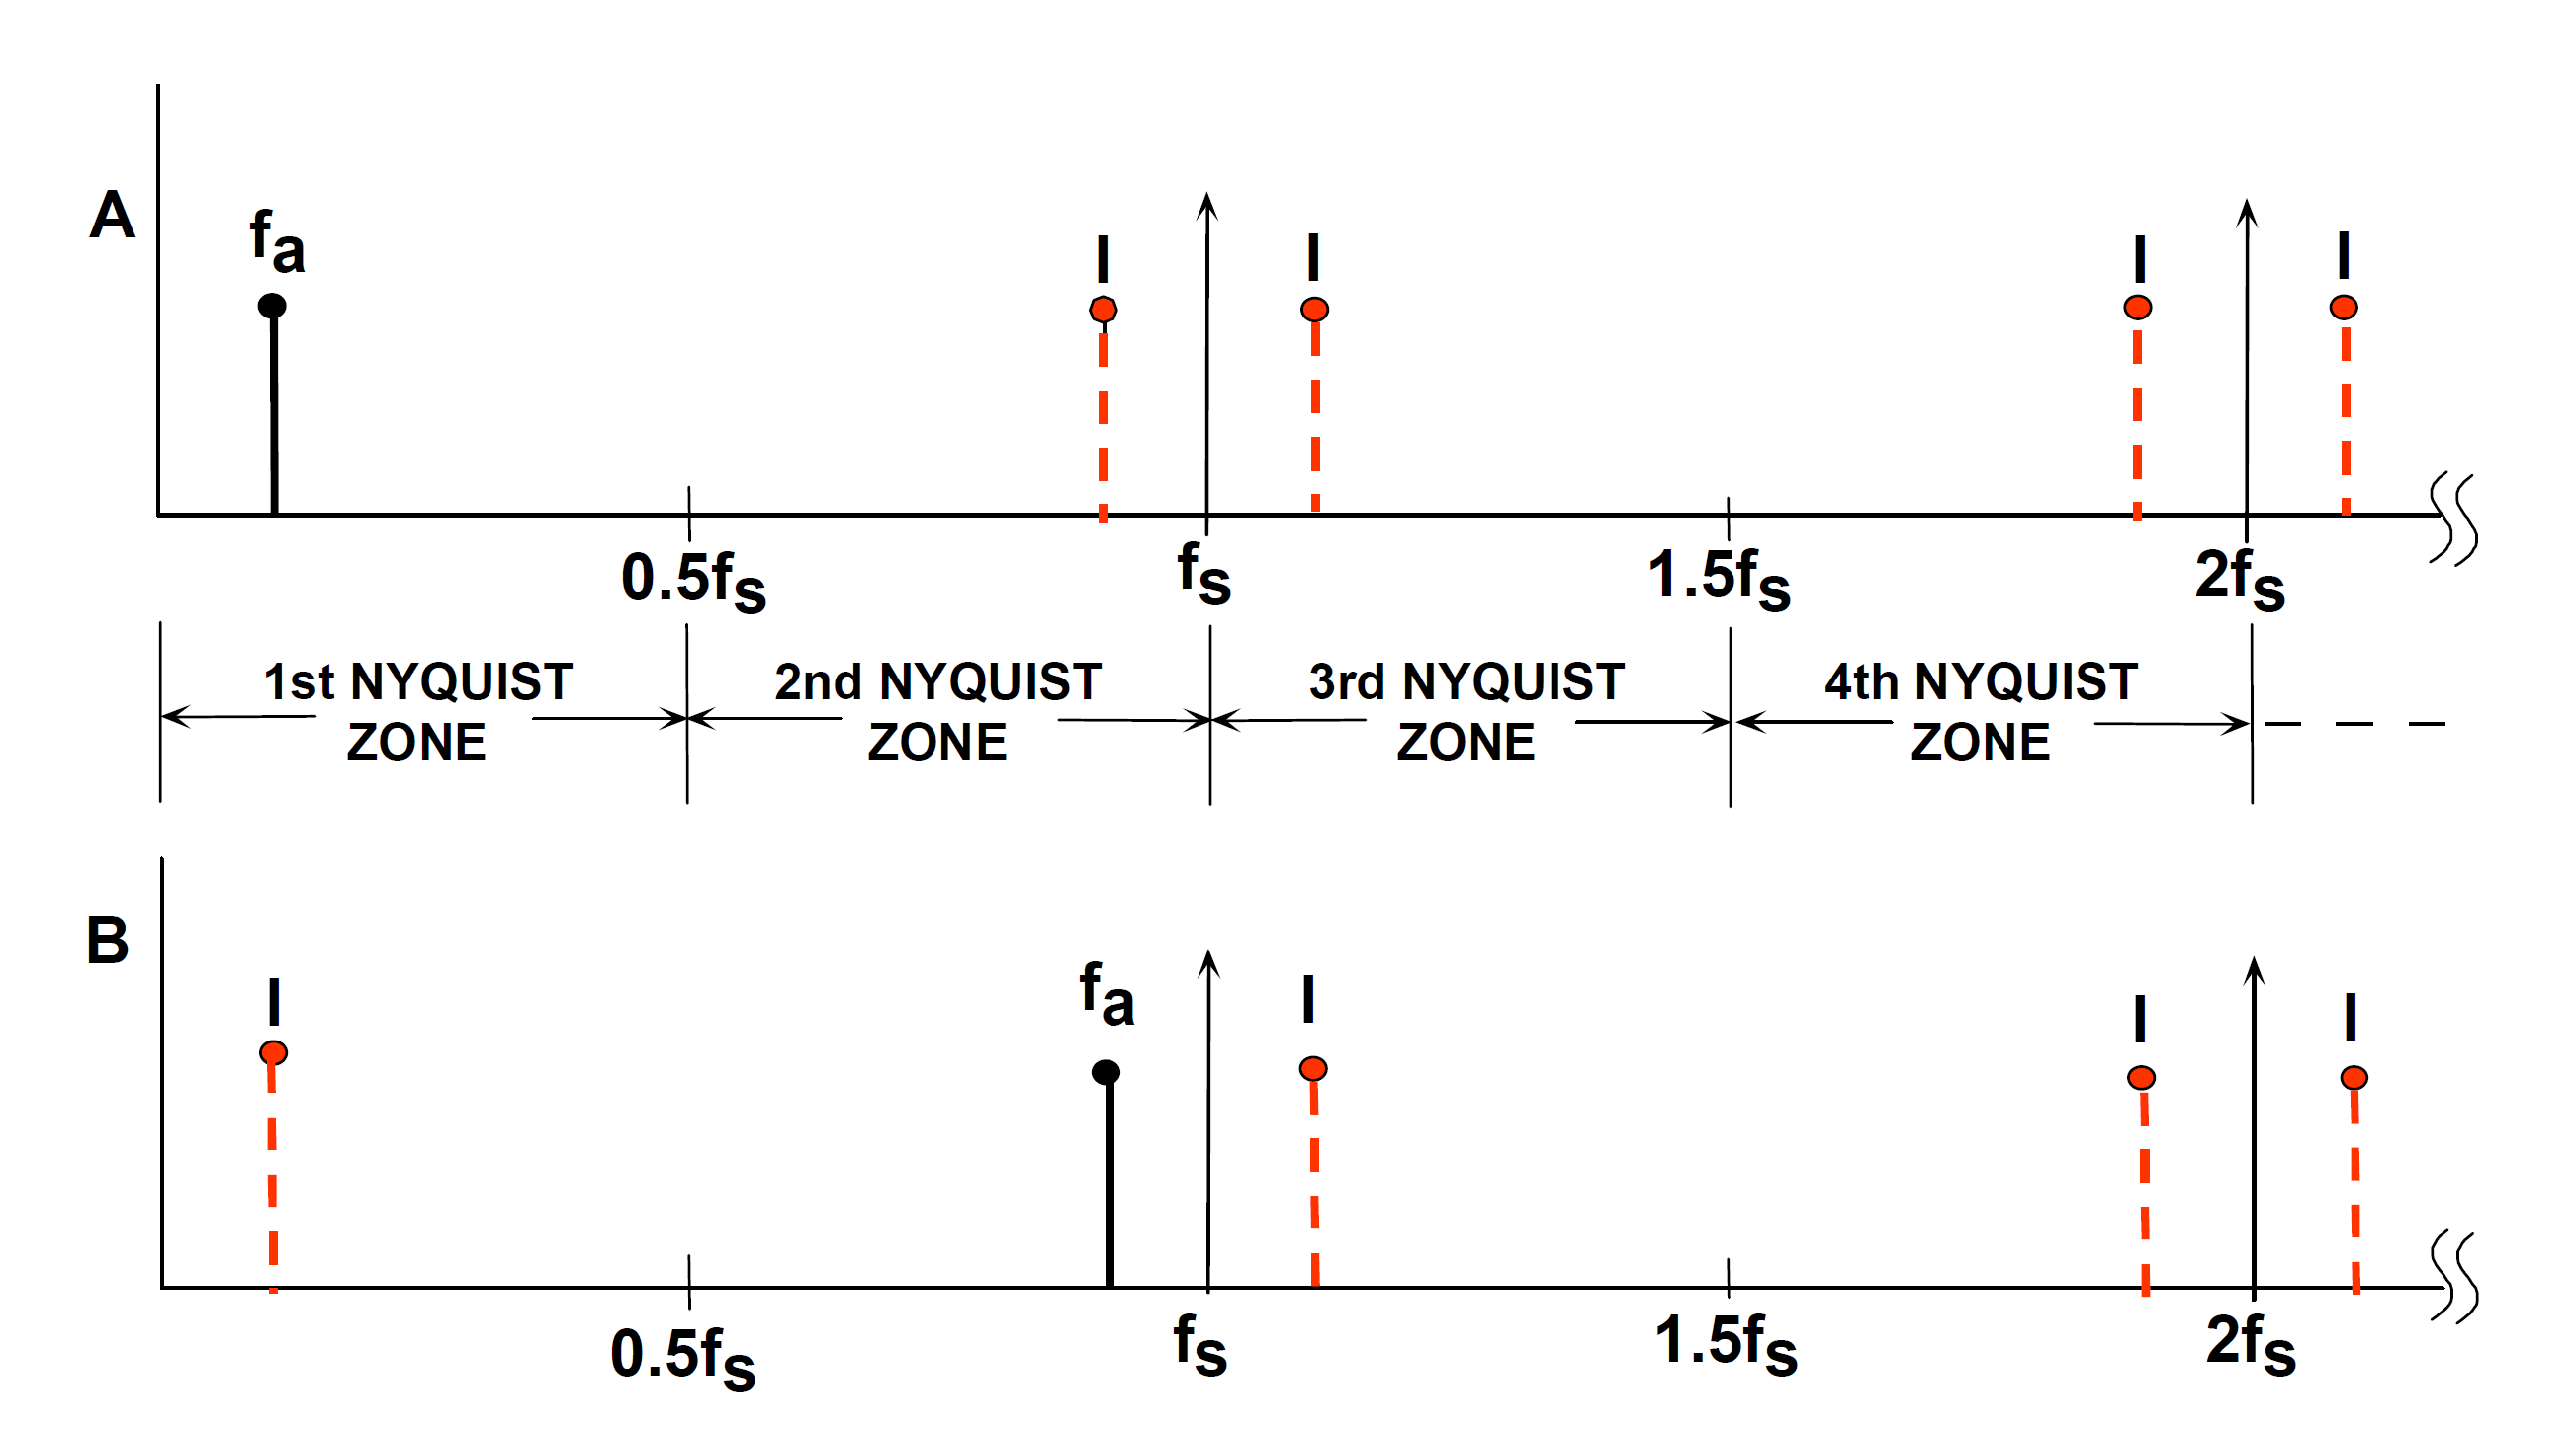
\includegraphics[width=\linewidth]{chap/02-theory/img/alias_f}  
		\caption{Sampling process visualized in frequency domain}
		\label{fig:alias_f}
	\end{subfigure}
	\begin{subfigure}{\textwidth}
		\centering
		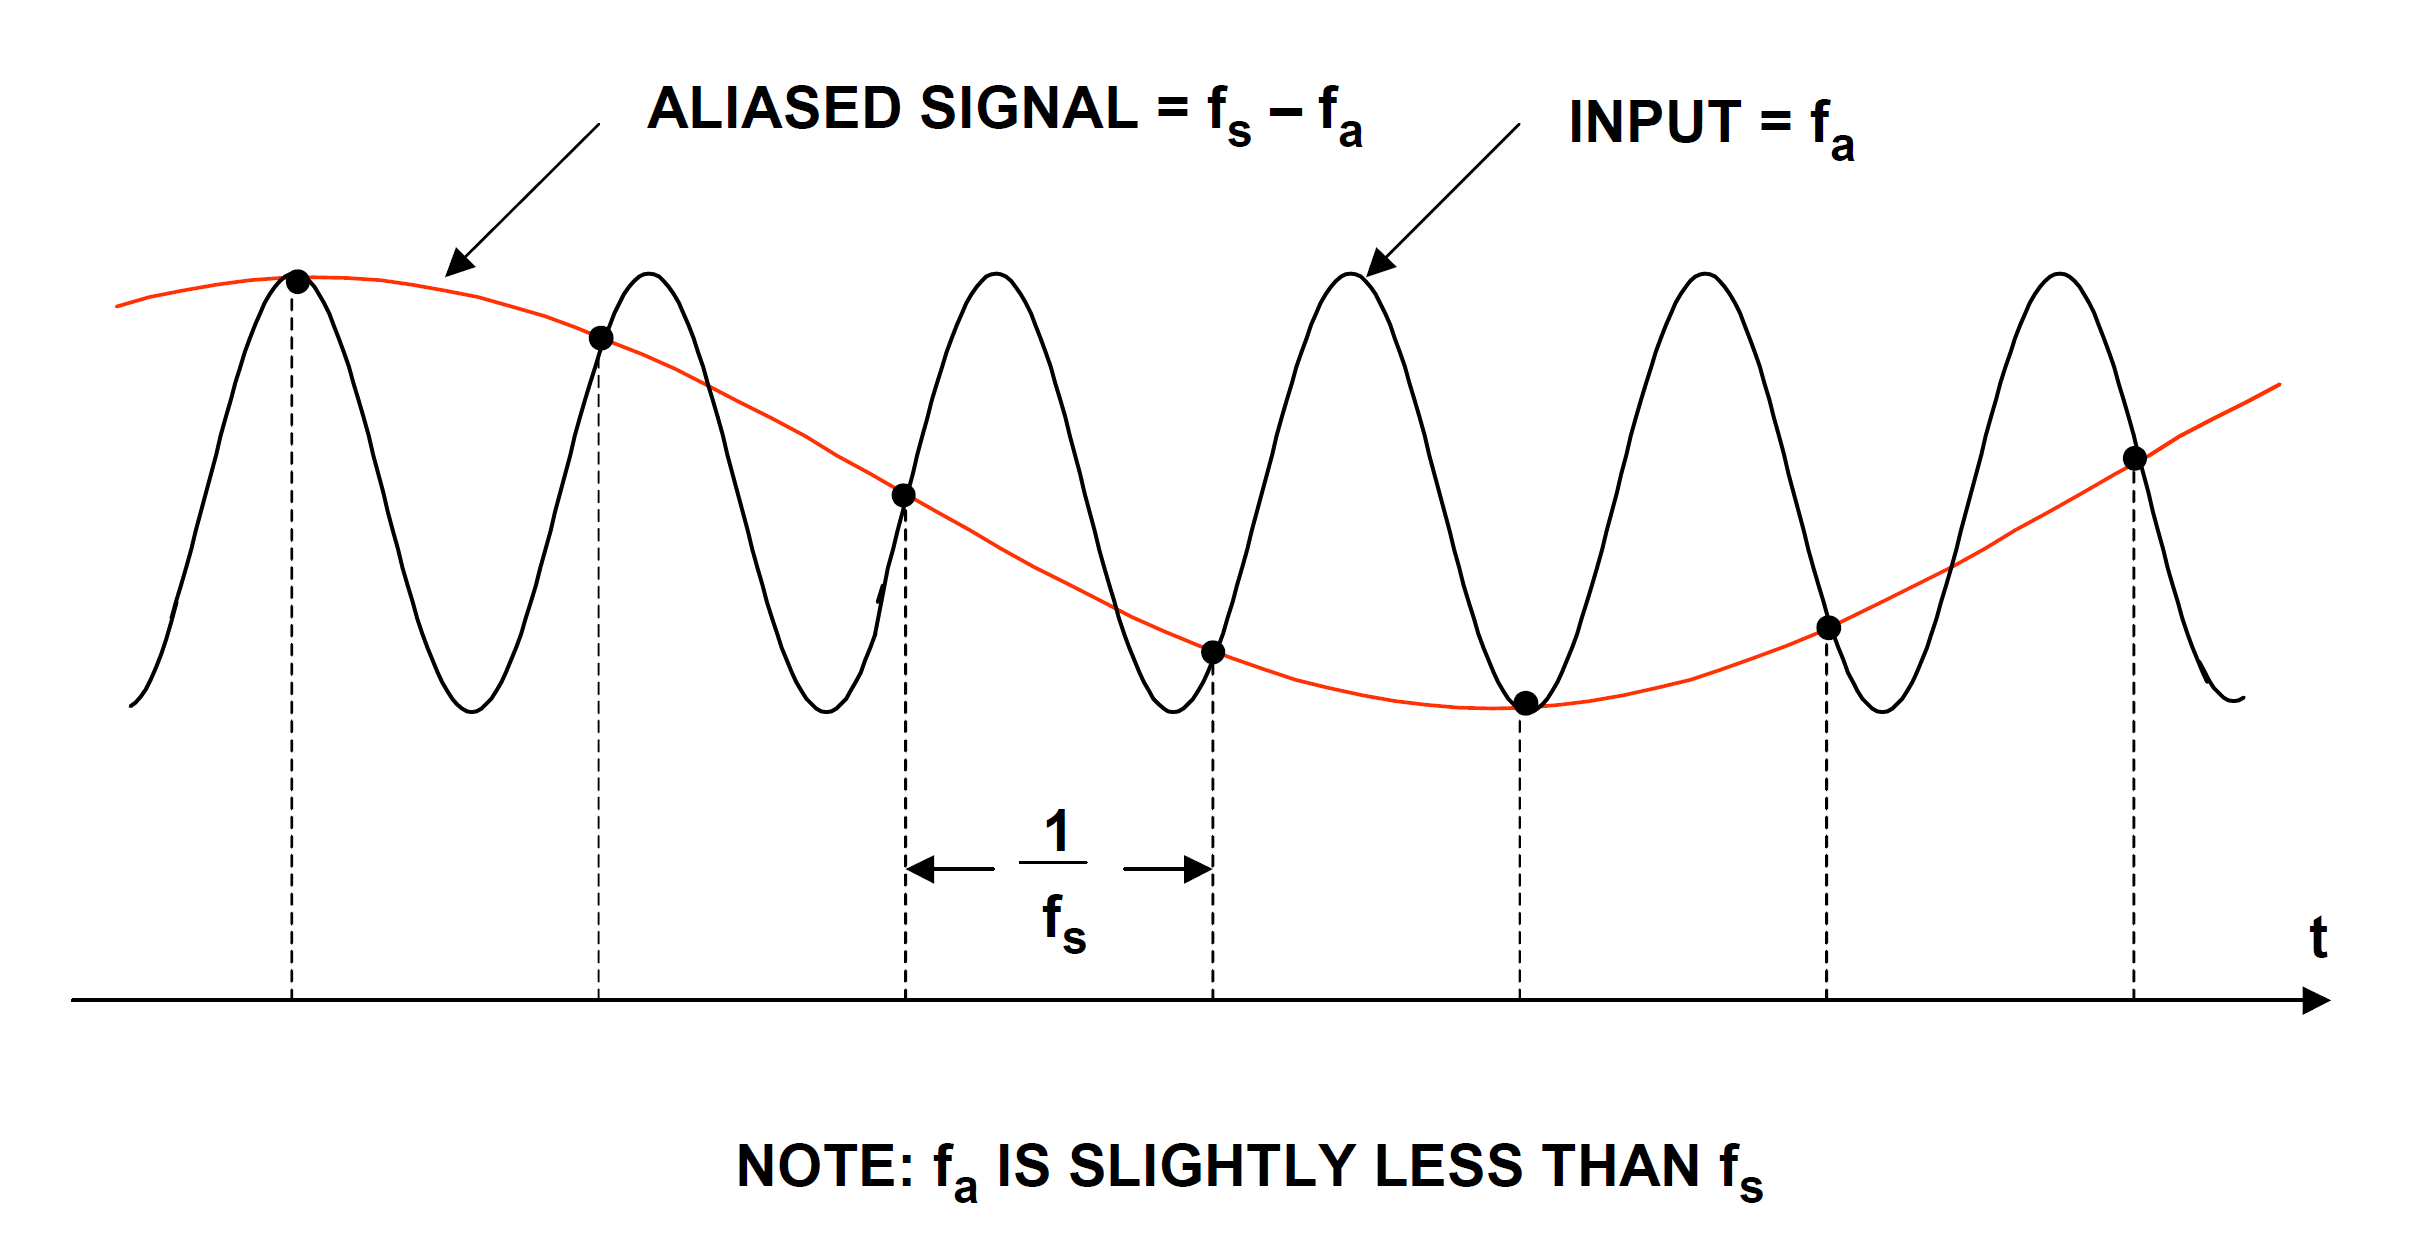
\includegraphics[width=\linewidth]{chap/02-theory/img/alias_t}  
		\caption{Effect of aliasing shown in time domain}
		\label{fig:alias_t}
	\end{subfigure}
	\caption[Aliasing]{Analog signal with frequency $f_a$ sampled at $f_s$ respecting (A) and not respecting (B) the Nyquist criteria (see \autoref{fig:alias_f}). \autoref{fig:alias_t} shows the effect of case B in time domain. \cite{walt}}
	\label{fig:aliasing}
\end{figure}
%todo low-pass filter to get B/2<f_s? maybe






   	\chapter{Architecture Of The New Readout-System - THERESA}
   			\begin{figure}[tbh]
	\centering
	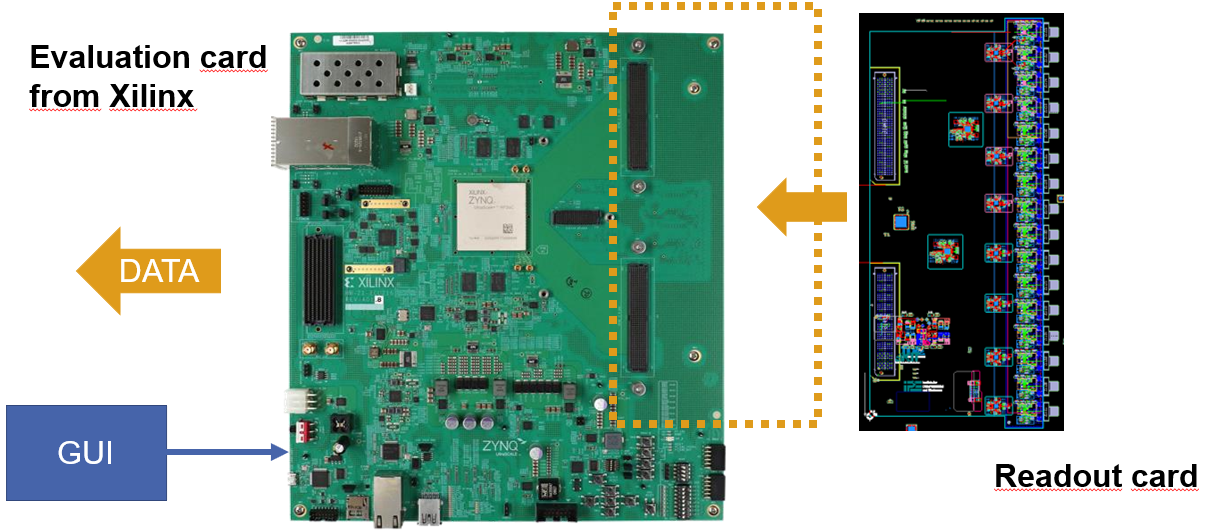
\includegraphics[width = \textwidth]{chap/04-work/img/concept_theresa}
	\caption{General concept of the new readout system}
	\label{fig:concept_theresa}
\end{figure}

\section{Optical part}
\section{Front-End Card}
\autoref{fig:theresa_scheme} shows the general schema of the sampling system, reduced to four channels for presentation purposes.
\begin{figure}[H]
	\centering
	\includegraphics[width = \textwidth]{chap/04-work/img/theresa_scheme.tikz}
	\caption{Placeholder: General schema of THERESA. For presentation purposes only four channels are shown.}
	\label{fig:theresa_scheme}
\end{figure}

\section{Readout Card}
\section{Selection Of The Card}\label{sec:selection}
When selecting the Readout Card, following criteria need to be considered:
\begin{itemize}
	\item Integrated \glspl{adc}
	\item Number, resolution and bandwidth of \glspl{adc}
	\item Peripheral connections
	\item Flexibility/Customization
	\item Suitable connectivity for high-data-throughput
\end{itemize}


\begin{figure}[tbh]
	\centering
	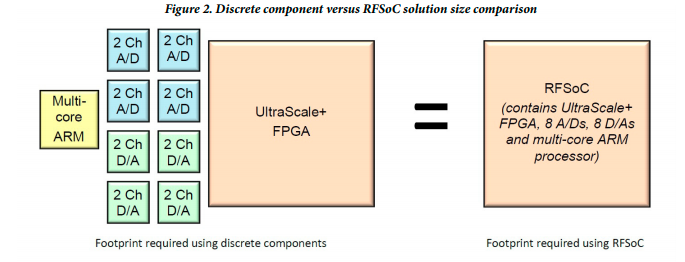
\includegraphics[width = \textwidth]{chap/04-work/img/footprint}
	\caption{Placeholder: Discrete vs IC}
	\label{fig:footprint}
\end{figure}
   	\chapter{Design Of The Front-End Sampling Card}
   			In the following, the process of designing the front-end sampling card is described. Designing a \gls{pcb} is a process of two steps: circuit design and layout design. The software tool used to cover both of these steps is PADS xDx Designer (for schematic capture) and PADS Layout/Router (for \gls{pcb} layout design) from Mentor Graphics (Siemens). 
\section{Schematics}
Without knowing which components are needed and how they are interconnected, it is impossible to manufacture any board, no matter how high or low the level of complexity is. The main purpose of a schematic is thus to provide a documentation about the necessary components and in which way they should be connected. Furthermore, a schematic provides a starting point for automatic translation of the components into the layout design tool.
During the creation of the schematics, the following points have to be taken into consideration:
\begin{itemize}
	\item Components: Which components are needed and what are the performance requirement? Especially for high-speed components carefully considering specifications like signal rise and fall times, jitter, skew, etc. is crucial to achieve the overall expected performance.
	\item Connection/Periphery: How many pins are available for peripheral connection? Many components have an interface for programming (e.g. \gls{spi}) which requires several pins. Especially for boards with a lot of components this can quickly become an issue.
	\item Signaling interfaces of the components: Additional circuitry might be needed for interfacing between two different components. Some signaling interfaces, like \gls{lvds}, require a specific voltage level, which might result in the need of voltage level translators.
	\item Common mode voltage: Keep in mind the different common mode voltages at input/output pins of different components and placing decoupling capacitors if needed.
	\item Filtering: Consider placing additional filtering for power supplies, as well as recommended filters from manufacturers of the components. 
	\item Power Supply: Choose suitable power supplies/voltage regulators. How many of them are needed?
	\item Size and Packaging: Packaging of the components. Obviously the size matters, as space on the board is limited. But package also introduces additional capacitance/inductance, which can be a problem for precise filtering circuits. 
	\item Power dissipation: Components, especially voltage regulators, might need coolers. This might not pose any problems for components which are located on the top side of the board. However, components on the bottom side might create an issue, if the designed \gls{pcb} should be mounted on another board.
	\item Availability: Check if the components are still available and if they can be delivered in the given project time.
\end{itemize}  
%todo irgendeine überleitung hinschreiben
 
\paragraph{Decoupling techniques}
Probably the most important part in schematics design is proper decoupling of power supplies, as \glspl{ic} require a stable voltage on the power supply pin for optimal performance. Any ripple\footnote{\textit{Ripple} is the \gls{ac}-voltage superimposed on an otherwise \gls{dc}-voltage.} or noise can substantially degrade the performance of the \glspl{ic}, i.e. by decreasing the noise margin\footnote{\textit{Noise margin} defines the difference between the useful signal and noise. A sufficient noise margin is necessary to guarantee that the output signal will still be correctly interpreted, even if some noise is added to the signal.}. Usually, manufacturers give information about proper decoupling circuits for their component in the data sheet. Is this not the case, there are basic rules of thumb which can be followed to ensure good decoupling. \cite{decouple}

Basically, two types of voltage variations on the power supply pin can be distinguished: low frequency and high frequency variation. Low frequency variation occurs e.g. due to devices (or parts of them) being enabled/disabled or in the event of data traffic or processing. The current draw during these occurrences can't be compensated immediately by the voltage regulator providing the supply voltage, which leads to voltage level sagging. Time frames of this noise vary in the range of milliseconds up to days. High frequency variation results from switching events in the device, occurring in the range of the clock frequency and the corresponding harmonics up to about \SI{5}{\giga \hertz}. Spikes due to \gls{emi} are also a source of high frequency variation and need to be compensated for. \cite{xilDecouple} 

Ideally, one capacitor, which acts like a low-pass filter, should be enough to mitigate these variations. A real capacitor however has parasitics and thus can in general not be modeled by a "pure" capacitive behavior, especially for high-frequency applications. Additional resistances and inductance need to be considered \cite{decouple}:
\begin{itemize}
	\item A parallel resistance $R_P$, which shunts the nominal capacitance ($C$), representing insulation resistance or leakage.
	\item A series resistance $R_S$, or \gls{esr}, which represents the plates and the leads of the capcitor.
	\item A series inductance $L_S$, or \gls{esl}, that models the inductance of the plates and leads of the capacitor.
	\item A parallel resistance and capacitance, $R_D$ and $R_C$, which model the effect called dielectric absorption. This denotes the phenomenon, that a capacitor which has been charged for a long time, doesn't fully discharge when briefly discharged. Dielectric absorption can be detrimental for high-precision use-cases, for power supply decoupling this effect doesn't have to be considered.
\end{itemize}
Considering all these effects leads to the equivalent circuit shown in \autoref{fig:real_cap}. It can be seen that this forms a RLC circuit, meaning the capacitor won't have the ideal behavior over all frequency range. Indeed, a real capacitor shows an impedance response as seen in \autoref{fig:esl_esr}, which resembles one of a band stop, rather than a low pass. Typical capacitive behavior is seen in region (I). Region (II) shows the influence of the \gls{esr}, which is why there is a residual impedance at the lowest point. Region (III) showcases the effect of the \gls{esl}. 
To "extend" the capacitive behavior over a wider frequency range, at least two capacitors are placed 

\tikzexternaldisable
\begin{figure}[tbh]
	\centering
	\includegraphics[width = .7\textwidth]{chap/04-work/img/real_cap.tikz}
	\caption[Capacitor equivalent circuit]{Equivalent circuit of a real capacitance (redrawn from \cite{decouple})}
	\label{fig:real_cap}
\end{figure}
\tikzexternalenable
\begin{figure}[tbh]
	\centering
	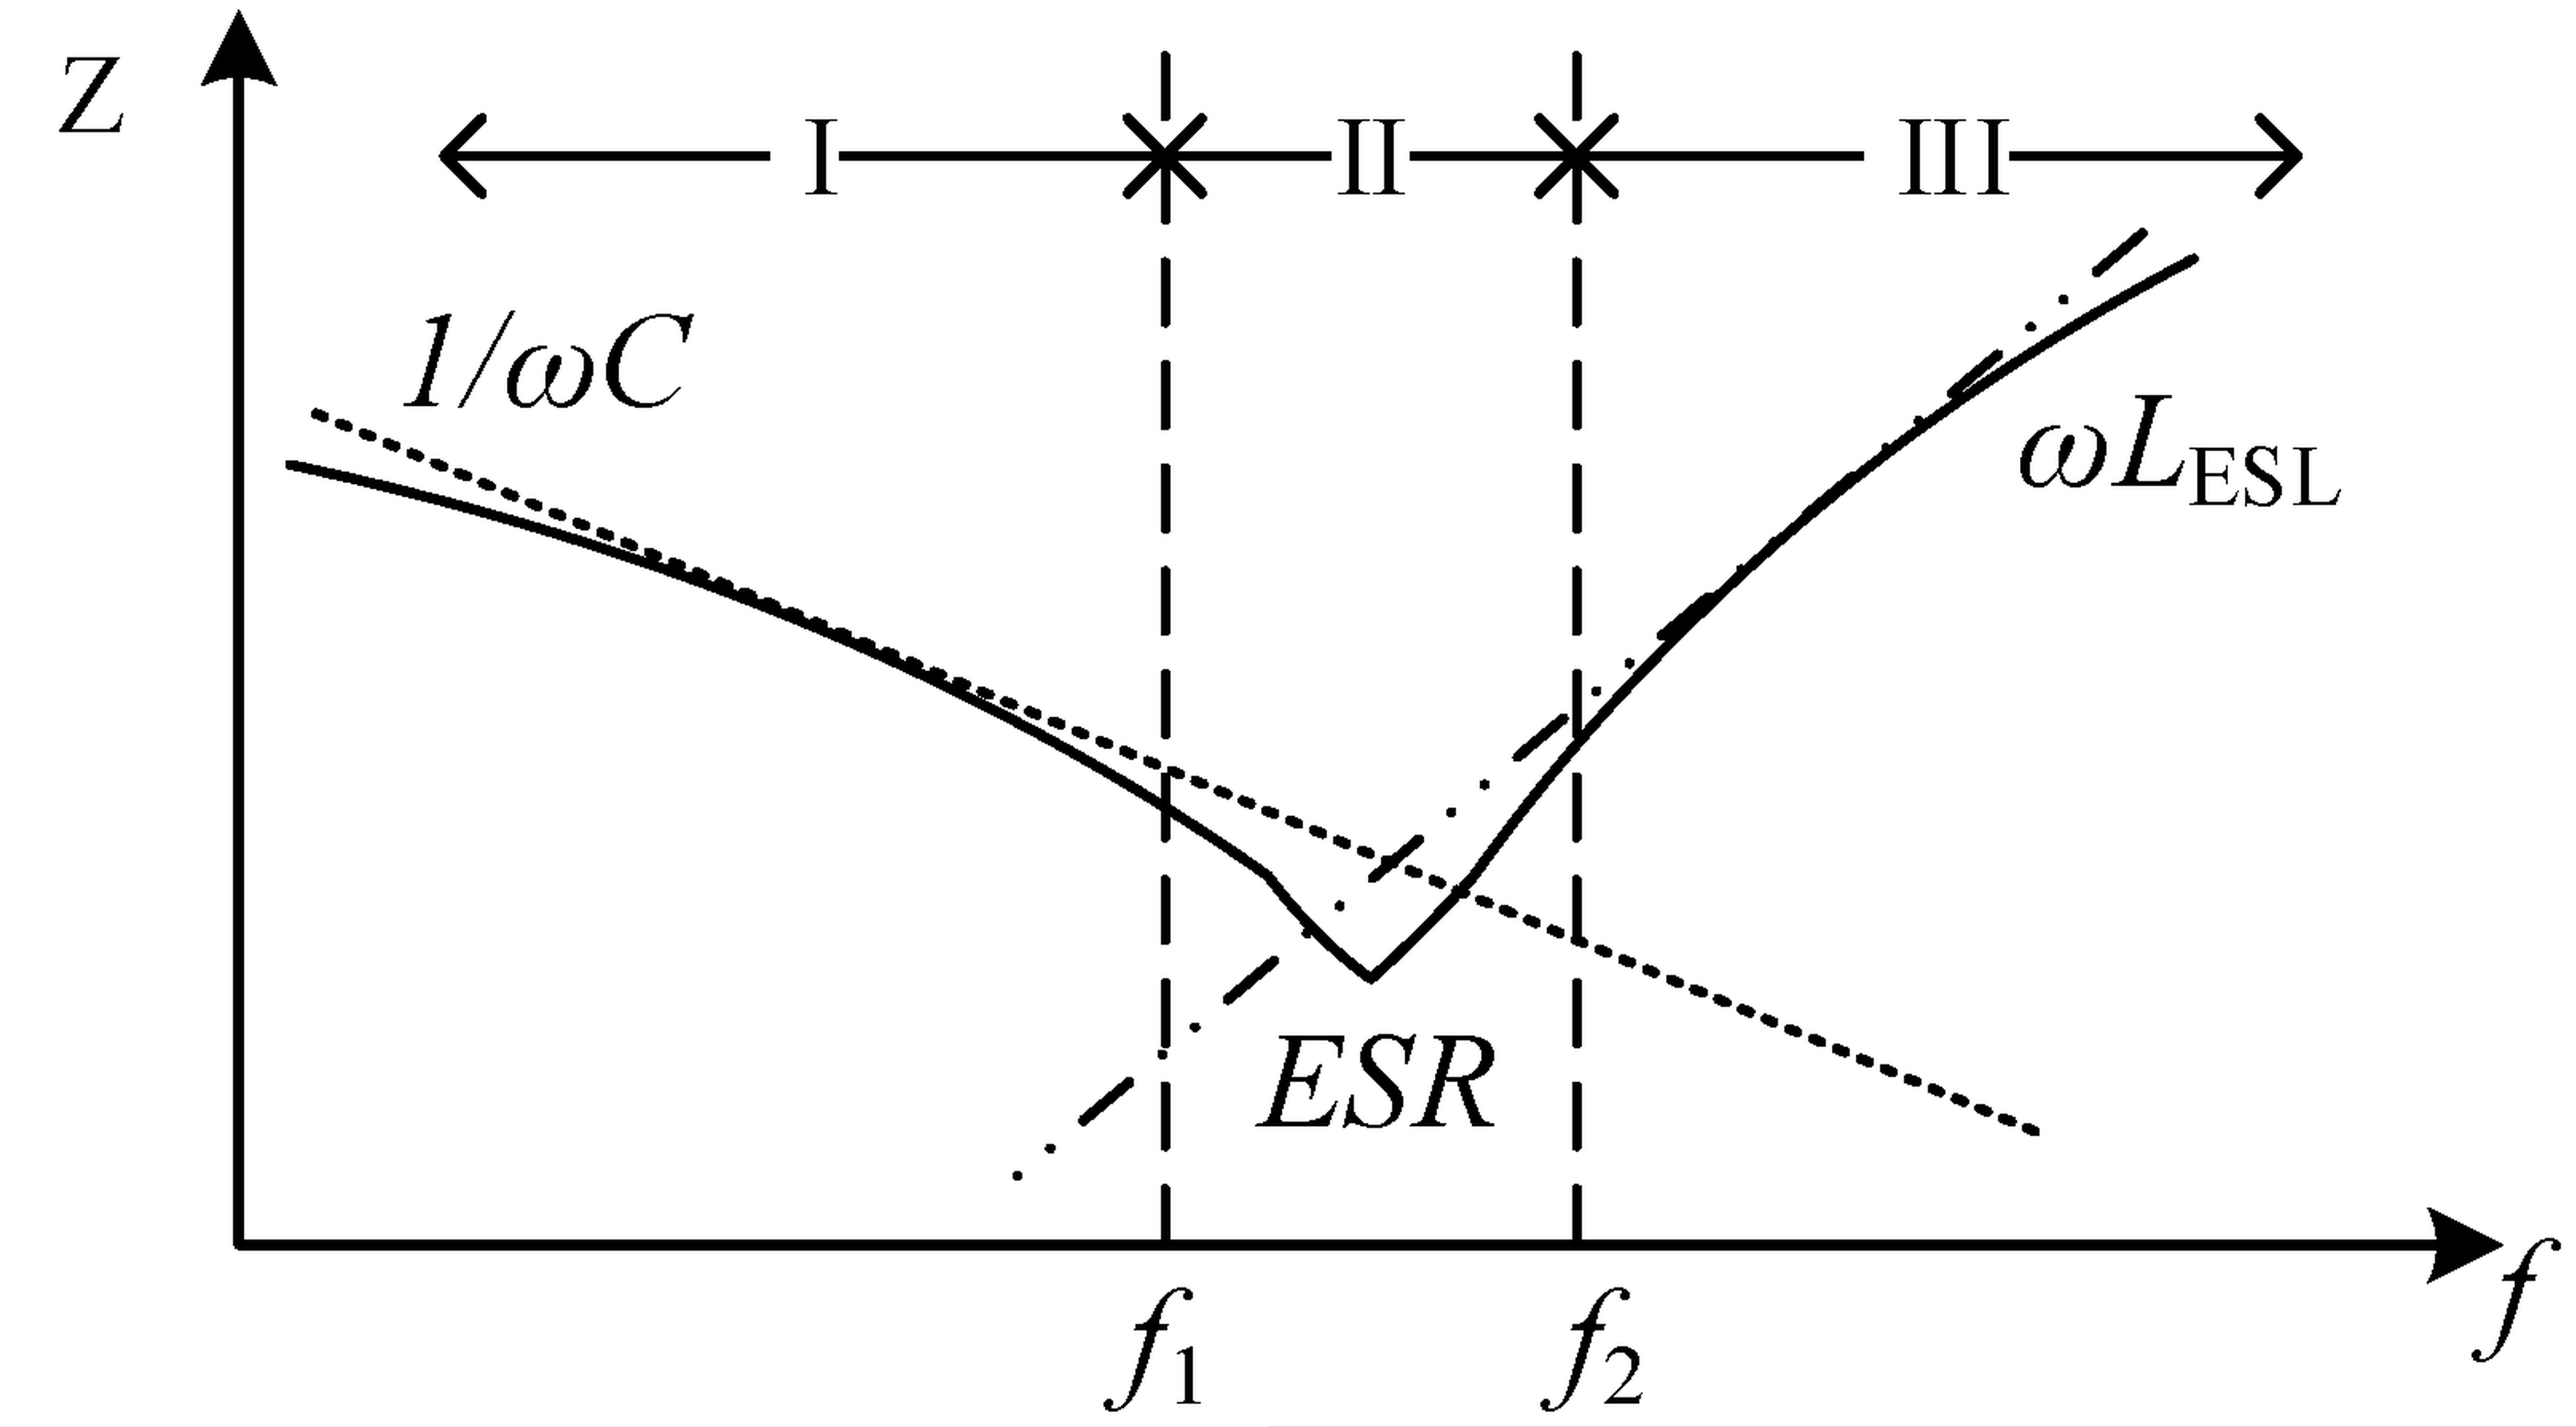
\includegraphics[width = \textwidth]{chap/04-work/img/esl_esr}
	\caption[Impedance response of a real capacitor]{Qualitative impedance response of a real capacitance \cite{Dang2020}}
	\label{fig:esl_esr}
\end{figure}


To deal with the low frequency variation, a large capacitor (typical values: 10 - \SI{100}{\micro \farad}) is placed next to the chip, not more than \SI{5}{\centi \metre} ($\approx$ 2 inch.) away. The role of this capacitor is to be a charge supply for the instantaneous needs of the device, i.e. "taking the role" of the voltage regulator until the latter can adjust to the changed current draw. \cite{decouple}

A small capacitor (typical values: 0.01 - \SI{0.1}{\micro \farad}), placed as close as possible to the power pins of the component. This capacitor should bypass the high frequency variation on the power supply line. \cite{decouple}

All capacitors should be connected through via\footnote{See \autoref{ssec:pcb_structs}} or short trace to a large area, low impedance ground plane\footnote{See \autoref{ssec:pcb_structs}}. This way the inductance due to connection traces is minimized. \cite{decouple}

An optional ferrite bead in series with the supply pin keeps external high frequency from the device and the internally generated noise from the rest of the board. \cite{decouple}

\paragraph{Separating Analog and Digital Ground}
TODO


%todo maybe some more theory, e.g. that real capacitor has resistive and inductive components due to packaging, connection and dielectric. doesn't behave like a capacitor at high frequencies -> several capacitors needed to ensure capacitive behaviour at high frequencies

\subsection{Connectors}\label{sec:connectors}
The number and type of connectors is primarily defined by the read-out card, on which the sampling board is mounted. The different connector types serve different purposes, which can be organized into three categories.
\paragraph{Digital Control Signals}
For digital control signals (i.e. \gls{spi}, enable signals, ...) and clocking a VITA 57.4 FMC+ connector from \textit{SAMTEC} is used (see \autoref{fig:fmcp}). 

\gls{fmc} is a standard defined by \gls{vita} to provide a standard mezzanine card\footnote{A \gls{pcb} which is plugged on a plug-in board. \cite{mezzanine}} form factor, connectors, and modular interface to a \gls{fpga} located on a base board (carrier card).\cite{Seelam2009} The \gls{fmc}+ standard extends the pin count and throughput of the present high-speed interfaces. 

This connector provides 560 pins arranged in a 14x40 array, 80 of which are additional high-speed interfaces, located on either side of the connector (therefore this connector type is also called \gls{hspce} connector, as opposed to the HSPC connector which doesn't have additional rows). 160 of them are data-pins configurable by the user. They can be used as single-ended or differential pins. Clocking capable pins can be used to propagate clocking from the mezzanine to the carrier board. 

Furthermore, the connector provides pins for power supply from carrier board to mezzanine card \cite{fmc}:
\begin{itemize}
	\item VADJ: Voltage adjustable from 0 to \SI{3.3}{\volt} (max. \SI{4}{\ampere}, max. \SI{1000}{\micro \farad} capacitive load) 
	\item \SI{3.3}{\volt} (max. \SI{3}{\ampere}, max. \SI{1000}{\micro \farad} capacitive load)
	\item \SI{12}{\volt} (max. \SI{1}{\ampere}, max. \SI{1000}{\micro \farad} capacitive load)
\end{itemize}
%todo to table?

An assembly drawing of the connectors is shown in \autoref{fig:fmcp}.

\begin{figure}[tbh]
	\centering
	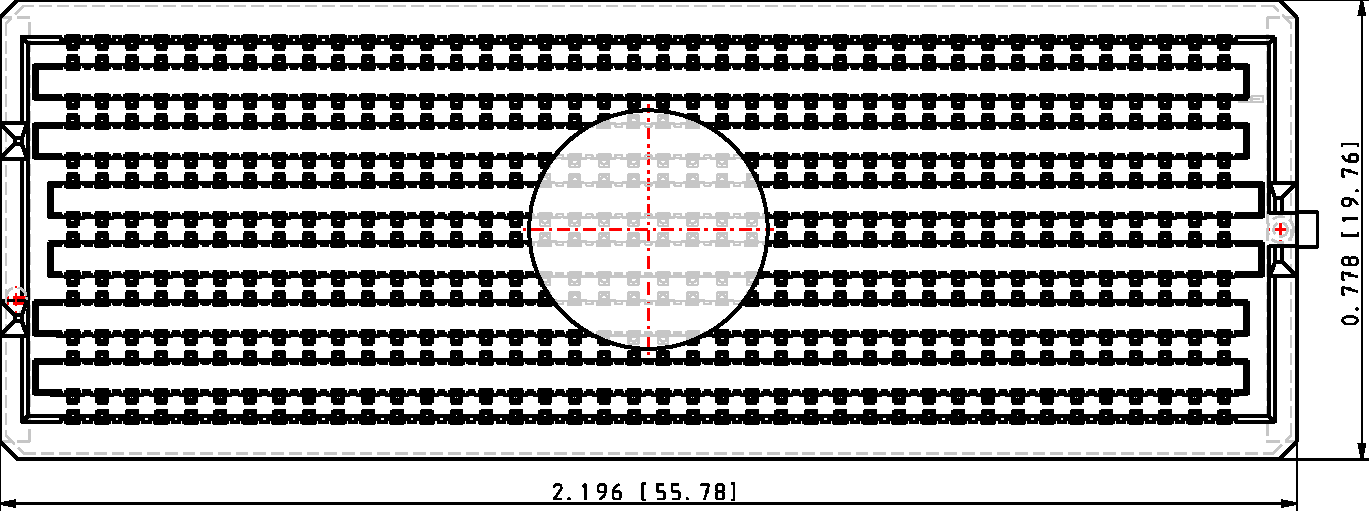
\includegraphics[width = 0.7\textwidth]{chap/04-work/img/fmcp.pdf}
	\caption[Rendering of FMC+ connector]{Part drawing of FMC+ connector \cite{fmcpic}}
	\label{fig:fmcp}
\end{figure}

\paragraph{Analog Signals}
The signal from the detector is provided to the \glspl{tha} through \gls{sma}\footnote{Coaxial \gls{rf} connector} \gls{rf} connectors from \textit{molex}, which are mounted at the edge of the board. \autoref{fig:sma} shows a 3D model of this connector type. 

\begin{figure}[tbh]
	\centering
	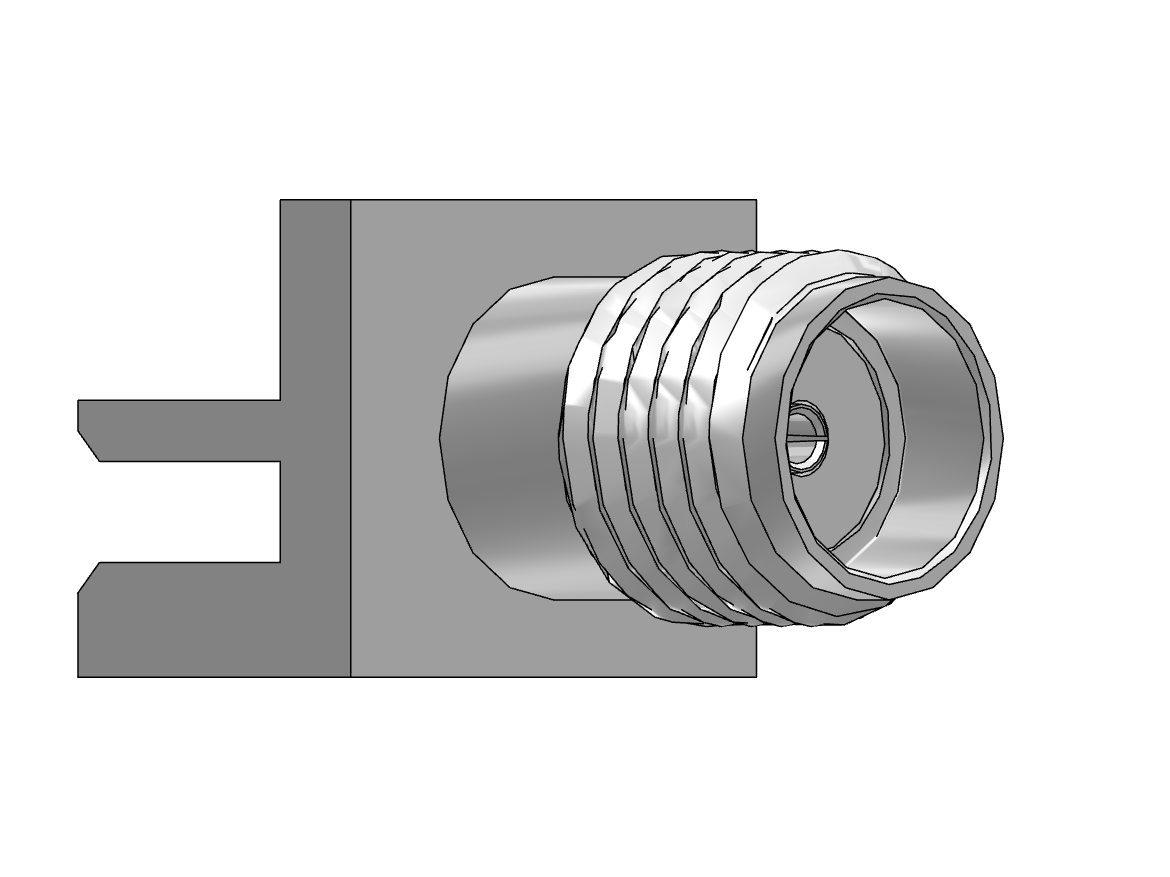
\includegraphics[width = 0.5\textwidth]{chap/04-work/img/sma}
	\caption[Edge-Mount RF SMA connector]{3D model of the edge-mount \gls{rf} \gls{sma} connector from \textit{molex} \cite{molex}}
	\label{fig:sma}
\end{figure}

On the read-out board two RFMC 2.0 (\gls{rf} Mezzanine Card) interface connectors are provided. The connectors used are LPAF (Low Profile Array, Female) connectors from \textit{SAMTEC} with 400 pins arranged in a 8x50 array. One is dedicated for transmitting signals from the mezzanine card to the on-board \glspl{adc}, the other provides the analog output from the on-board \glspl{dac}\footnote{A \gls{dac} translates digital values into an analog signal.} to the mezzanine card. On the sampling board, the "male" (LPAM) counterpart of the connectors is used (see \autoref{fig:lpam1}).

\begin{figure}[tbh]
	\centering
	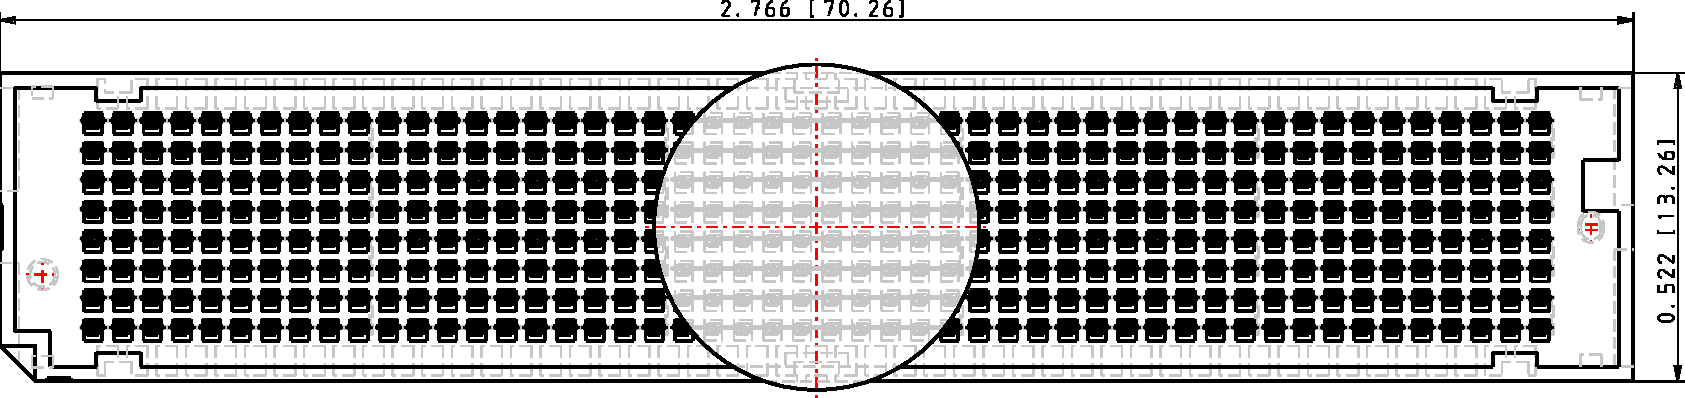
\includegraphics[width = \textwidth]{chap/04-work/img/lpam_50_top.pdf}
	\caption[LPAM 8x50 connector]{Part drawing of a LPAM 8x50 connector}
	\label{fig:lpam1}
\end{figure}


\paragraph{Clock Signals}
The clock from the \glspl{pll} on the sampling board are propagated in different ways. The reference clock for the \gls{fpga} is propagated through the \gls{fmc}+ connector. Clocking for \glspl{adc} and \glspl{dac} is provided through a 6x20 LPAM connector (see \autoref{fig:lpam2}). For interleaving 


\begin{figure}[tbh]
	\centering
	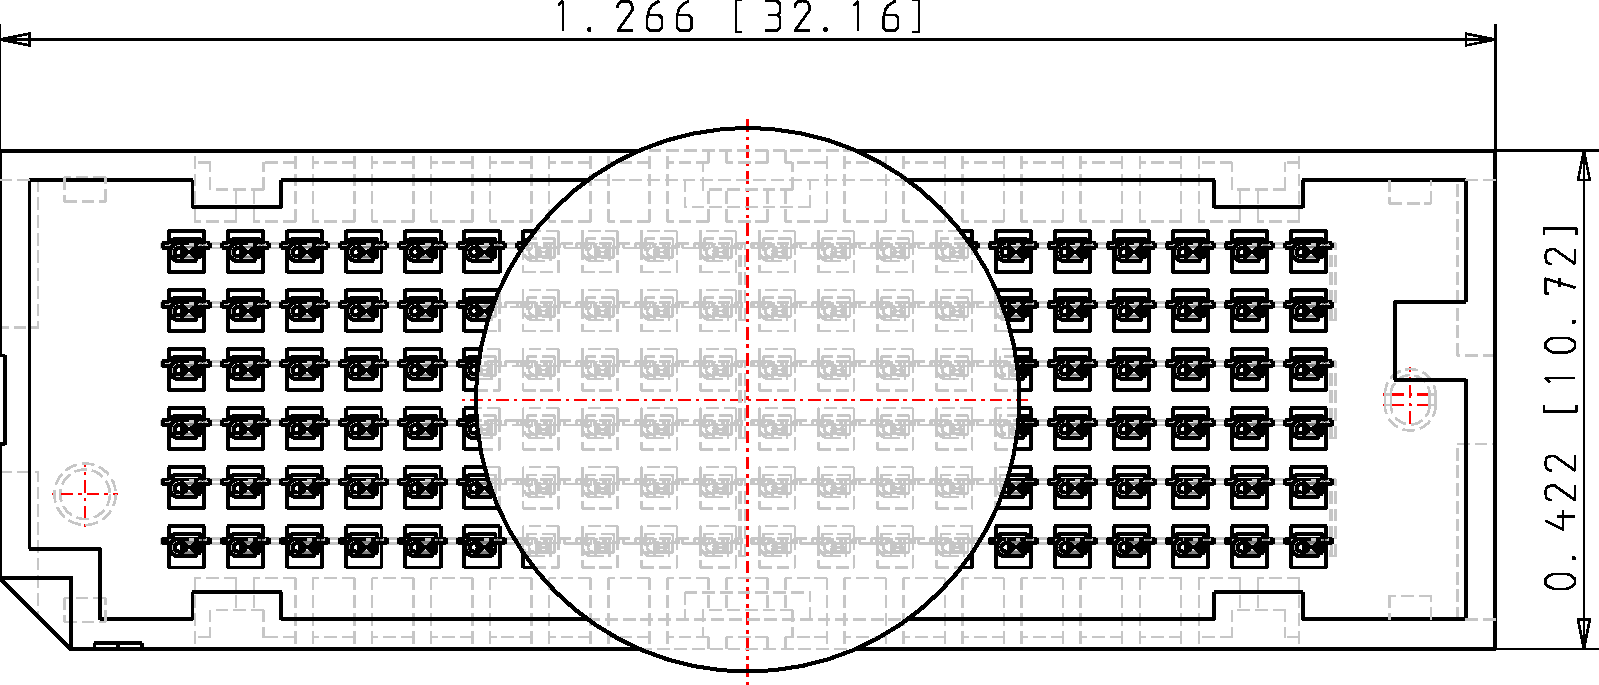
\includegraphics[width = 0.7\textwidth]{chap/04-work/img/lpam_20.pdf}
	\caption[LPAM 6x20 connector]{Part drawing of LPAM 6x20 connector}
	\label{fig:lpam2}
\end{figure}

%todo other pictures of connectors? maybe photos/renderings are better?



\subsection{Sampling-Channel}
The sampling channel consists of the \gls{tha}, which is driven by a delay chip. 

\paragraph{Track-And-Hold-Amplifier}
The \gls{tha} used is the same as in \gls{kapture}. The component was chosen such that jitter lies in the range of hundreds of femtoseconds. \cite{caselle2013}
According to the data sheet \cite{hmc5640}, the component shows the characteristics shown in \autoref{tab:hmc5640}.
\begin{table}[tbh]
	\caption[HMC5640 Characteristics]{Specifications of the HMC5640 \gls{tha}}
	\label{tab:hmc5640}
	\begin{minipage}{\textwidth}
		\centering
		\begin{tabularx}{\textwidth}{Xcccc}
			\toprule
			\textbf{Parameter} & \textbf{Min} & \textbf{Typ.} & \textbf{Max} & \textbf{Unit}\\
			\midrule
			\textbf{Analog Inputs} &&&& \\
			Differential \gls{fs} Range & & 1 & & Vpp\footnote{Volt peak-to-peak}\\
			Common mode voltage & -0.1 & 0 & 0.1 & V\\[0.3cm]
			\textbf{Clock Inputs} &&&&\\
			DC Differential High Voltage (Track Mode) & 20 & 40 & 2000 & mV\\
			DC Differential Low Voltage (Hold Mode) & -2000 & -40 & -20 & mV\\
			Common mode voltage & -0.5 & 0 & 0.5 & V\\[0.3cm]
			\textbf{Analog Outputs} &&&&\\
			Differential \gls{fs} Range &  & 1 && Vpp\\
			Common mode voltage & & 0 & & V\\[0.3cm]
			\textbf{Track-to-Hold/Hold-to-Track Switching} &&&&\\
			Aperture Delay & & -6 &  & ps\\
			Random Aperture Jitter (\gls{fs}, \SI{1}{\giga \hertz}) & & < 70 & & fs\\
			Settling time\footnote{\textit{Settling time} is the interval between the internal track-hold transition and the time when the output signal is settled within the specified value.} (to \SI{1}{\milli \volt}) &	&  116 & & ps \\
			\bottomrule
		\end{tabularx}
	\end{minipage}
\end{table}

As the analog input to the \gls{tha} is single-ended, a \SI{50}{\ohm} termination on the unused input pin has been added, as recommended in the data sheet.\cite{hmc5640}
%todo the siunitx omega looks kinda ugly   	explain transmission lines and termination?

At the power pins, decoupling capacitors and a ferrite bead  were placed. The \gls{tha} is a crucial component, as it samples the detector signal, therefore any possible noise should be reduced to a minimum.

\begin{figure}[tbh]
	\centering
	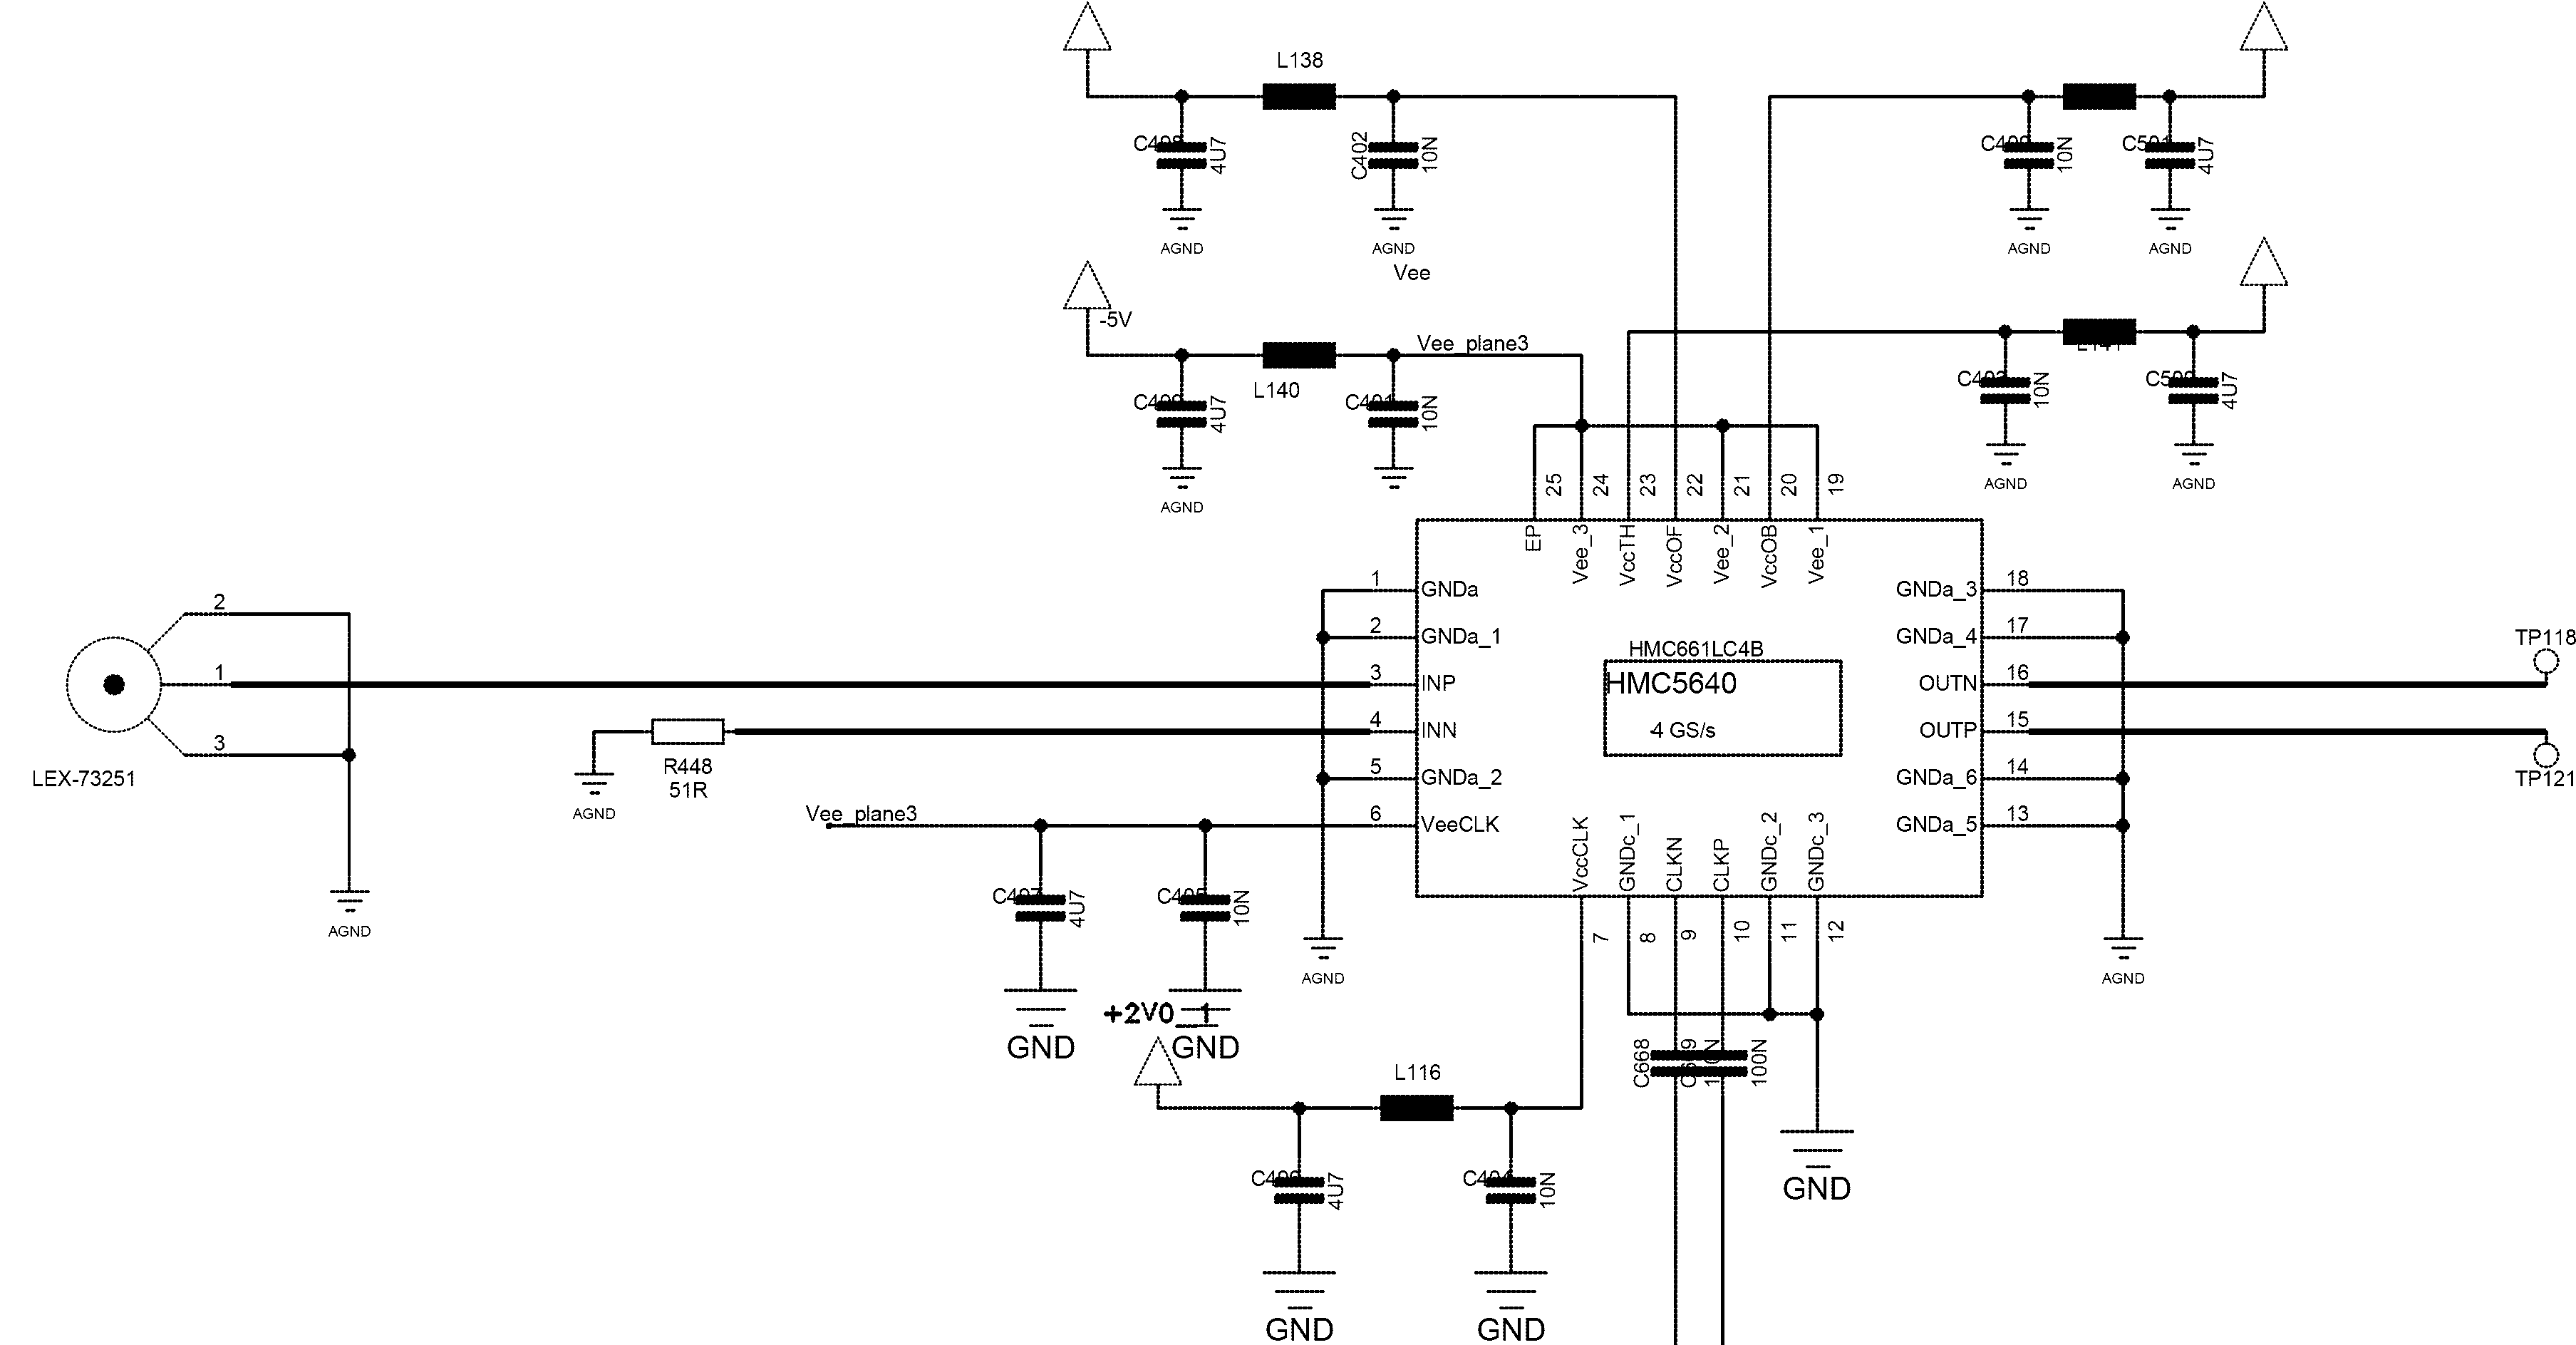
\includegraphics[width = \textwidth]{chap/04-work/img/hmc5640}
	\caption[HMC5640 THA Schematic]{HMC5640 \gls{tha} schematic}
	\label{fig:hmc5640}
\end{figure}
%todo better picture/somehow improve this BS
%todo maybe only a pic of the component itself


\paragraph{Delay Chip}
The delay chip is used to create a delay in the clocking signal, which then goes to the \gls{tha} chip. For the selection of the delay chip, the most important characteristic, apart from jitter, is the delay step size and delay range. 

The delay step size must be small enough, such that the \gls{adc} interleaving technique \autoref{sssec:time-interleaving} can be implemented. The \glspl{adc} on the read-out card sample at a maximal sample rate of \SI{2.5}{\giga \sample \per \second}, meaning during the time
\begin{equation}
	t_s = \frac{1}{\SI{2.5}{\giga \sample \per \second}} = \SI{400}{\pico \second}
\end{equation}
all 16 \glspl{adc} have to be clocked one time. This means, a delay step can not be greater than $\SI{400}{\pico \second}/16 = \SI{25}{\pico \second}$.

With the HMC856 programmable delay chip from \textit{Analog Devices}, which is also used for the \gls{kapture} sampling, a minimal step size of \SI{3}{\pico \second} \cite{hmc856} is possible. However, one draw-back is the maximal delay range of \SI{100}{\pico \second}. Considering a signal, which is stretched over several nanoseconds, this range limits the possibility to freely chose the resulting timing resolution. The major problem is the programming interface of the chip, which consists of five differential \gls{cml} inputs. This means, one chip already takes up 10 pins. For in total 16 necessary delay chips, this results in 160 pins occupied only by the delay chips. This occupies all pins of the \gls{fmc}+ connector (see \autoref{sec:connectors}) available for the user. 

A better candidate is the dual channel programmable delay chip NB6L295 from \textit{ON Semiconductor}. This chip provides two programmable delay channels, therefore effectively reducing the chip count by half. With a delay step size of \SI{11}{\pico \second} it is still suitable for the targeted interleaving method, covering a total delay range from \SI{3.2}{\nano \second} to \SI{8.8}{\nano \second} per delay channel. The chip is programmed via \gls{sdi}, which only requires 3 pins and one enable pin. Thus, the total number of pins used by the delay chips is $4\cdot8 = 32$, which is a significant reduction compared to the HMC856.

\begin{figure}[tbh]
	\centering
	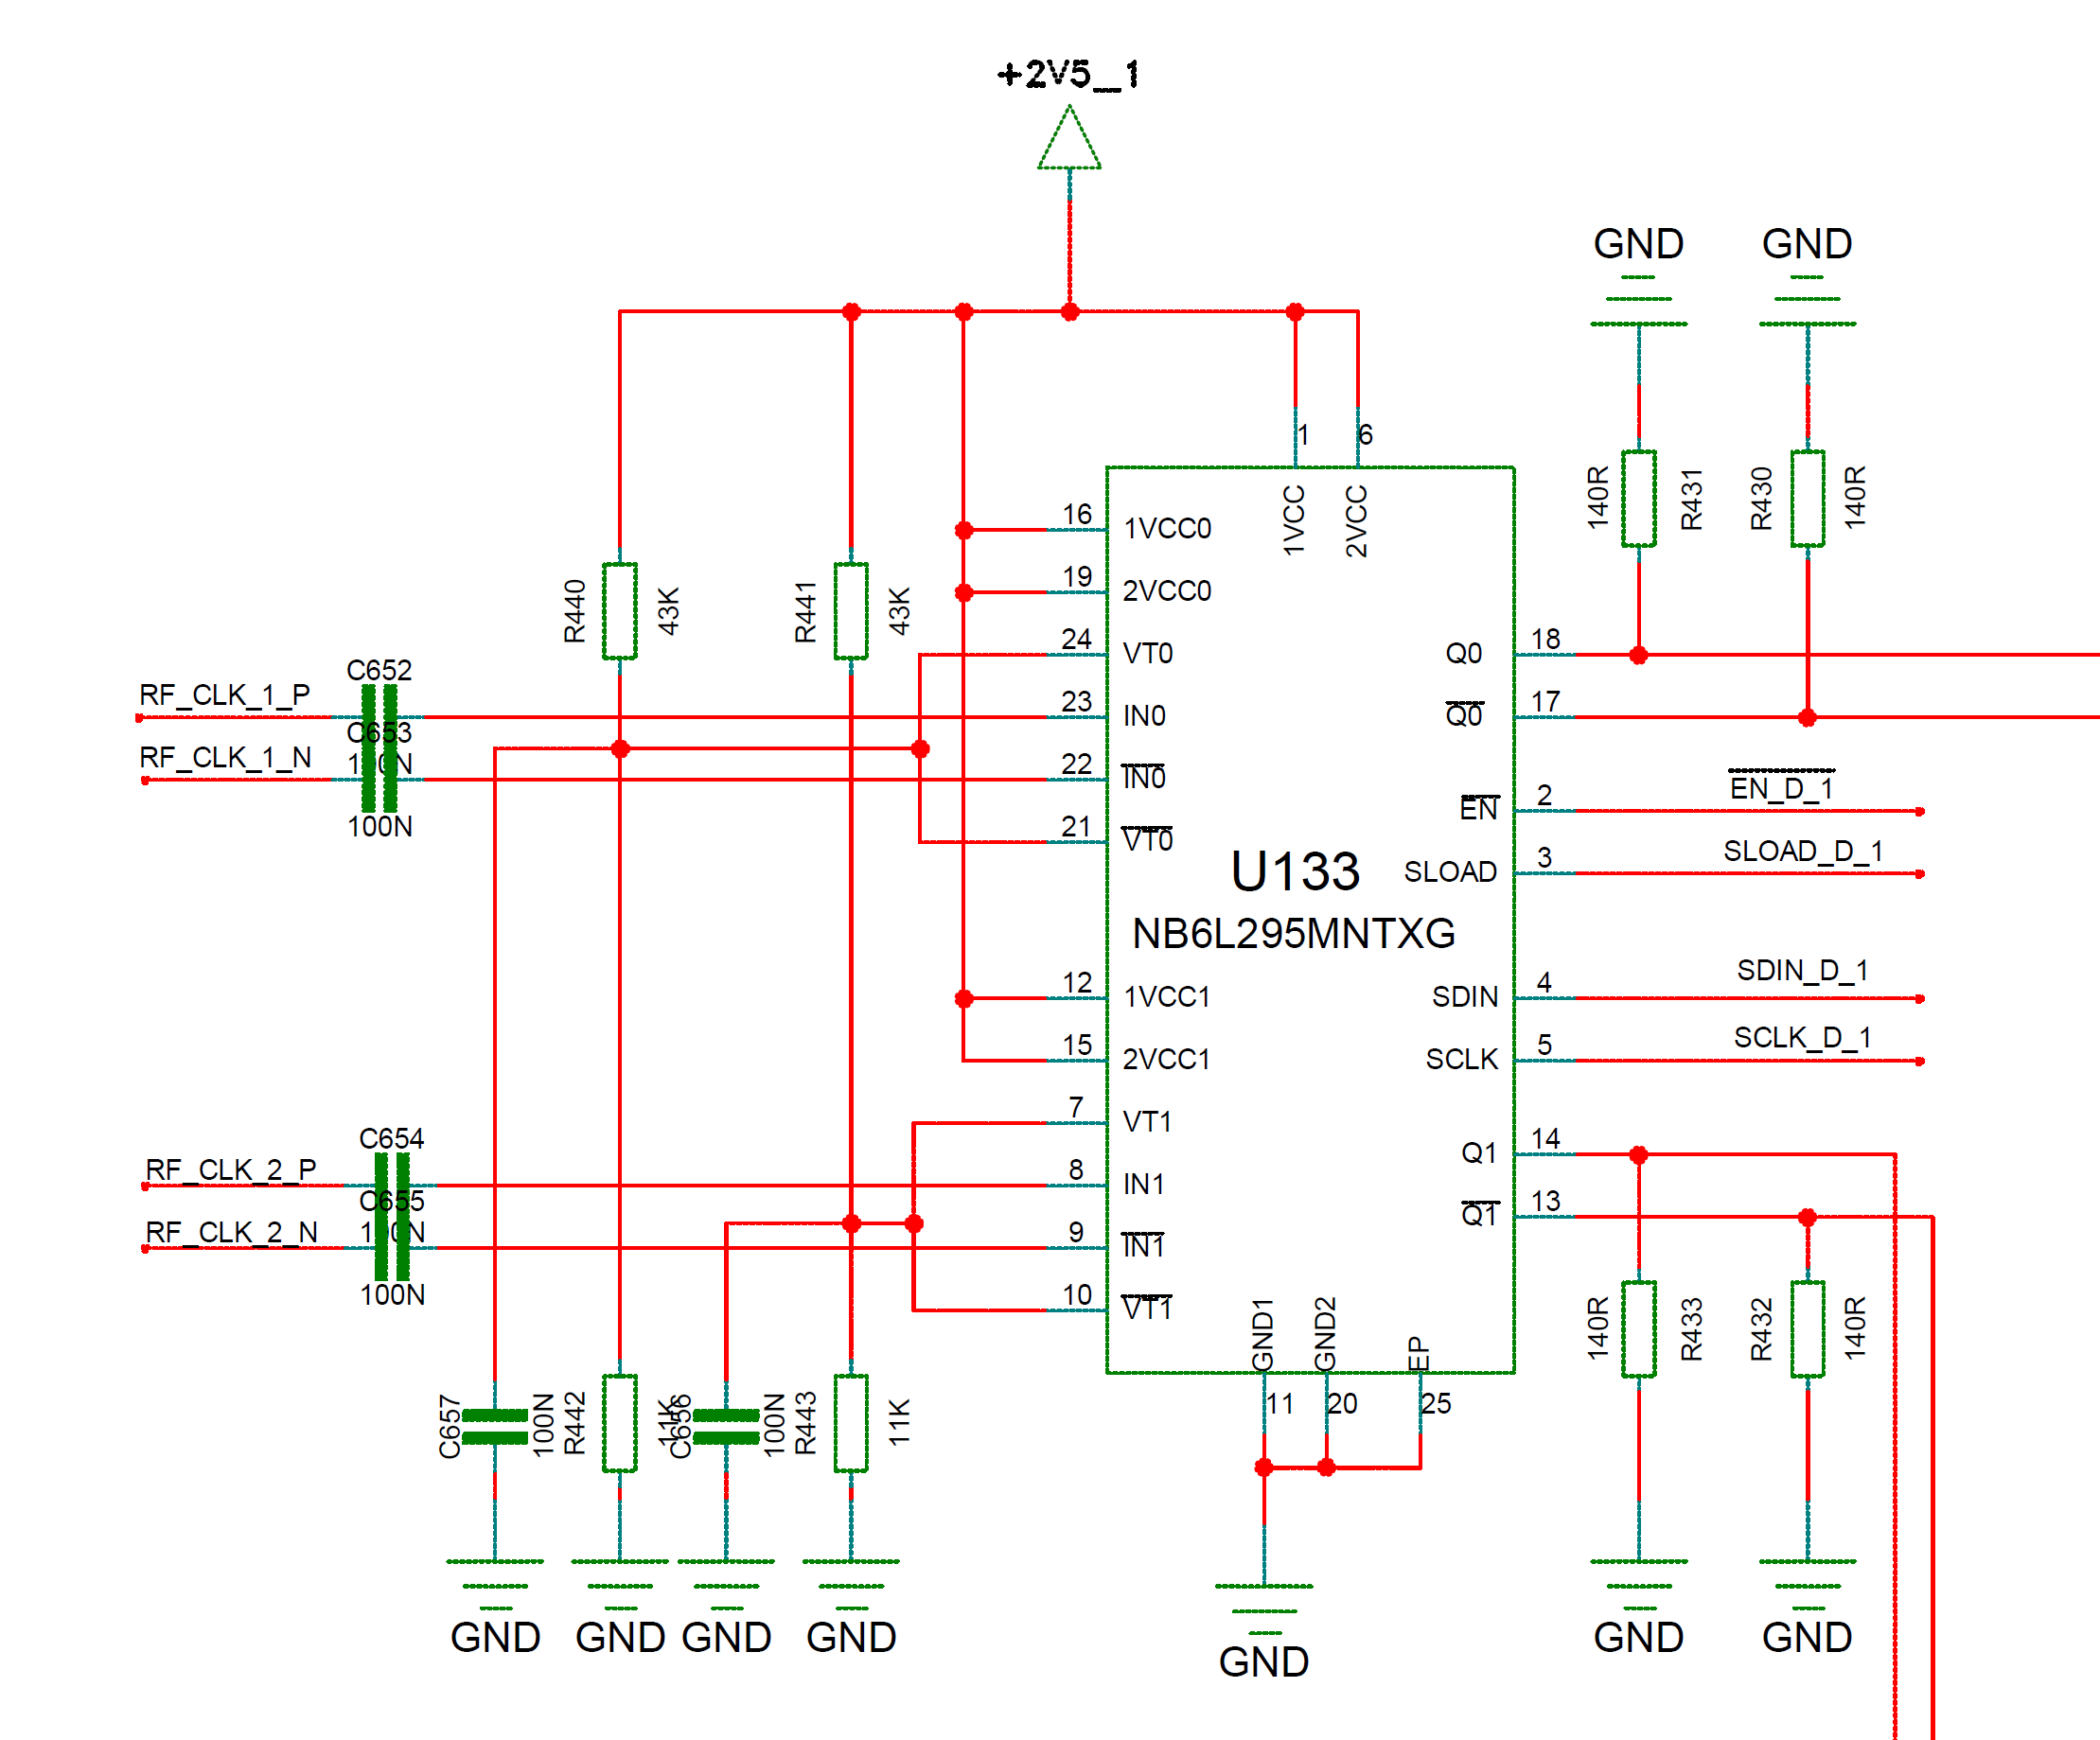
\includegraphics[width = \textwidth]{chap/04-work/img/delay_chip}
	\caption[NB6L295 Delay Chip Schematic]{NB6L295 schematic}
	\label{fig:nb6l295}
\end{figure}

\paragraph{Outputs}
The output of the delay chip is using a \gls{lvpecl} signaling interface, which is based on an open-emitter topology (see \autoref{fig:lvpecl}). This requires a path to \gls{dc}, which is achieved by adding \SI{140}{\ohm} resistors.
\begin{figure}[tbh]
	\centering
	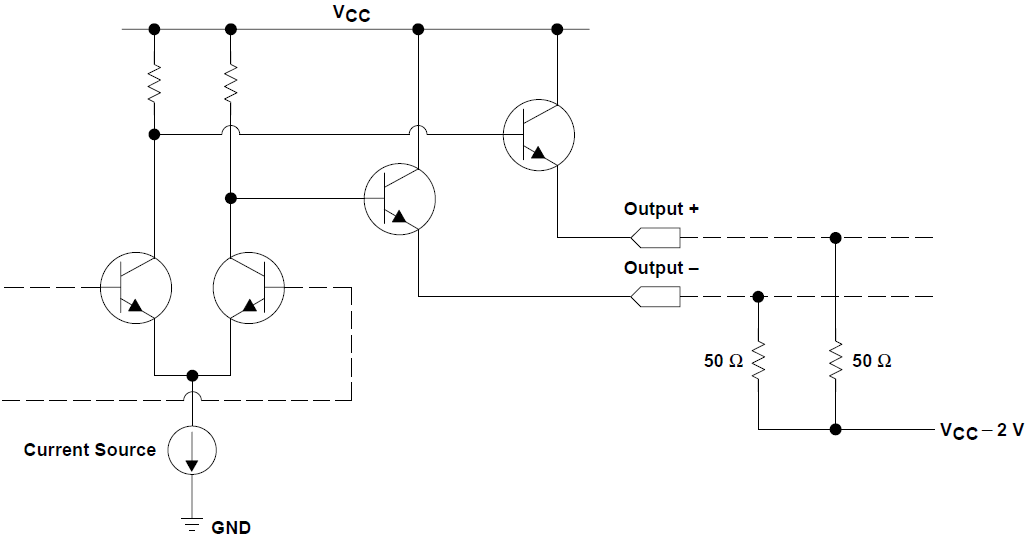
\includegraphics[width = \textwidth]{chap/04-work/img/lvpecl}
	\caption[LVPECL driver topology]{LVPECL driver topology. Left side shows the emitter-follower based driver. On the right, an example biasing with resistors is shown. \cite{lvpecl}}
	\label{fig:lvpecl}
\end{figure}
%todo to tikz

As the output will be connected to the \gls{tha}, it is necessary to check the compatibitility of the maximum amplitude and common mode. According to the data sheet \cite{NB6L295}, the voltage level of the output can vary between  $V_{cc} - 1825$ mV and $V_{cc} - 825$ mV (see \autoref{tab:nb6l295}).  Maximal voltage amplitude acceptable by the \gls{tha} inputs is \SI{2000}{\milli \volt} (see \autoref{tab:hmc5640}). When using a supply voltage of $V_{cc} = \SI{3.3}{\volt}$, which is e.g. provided by the read-out card through the \gls{fmc}+ connector, this leads to a maximum output level of \SI{2475}{\milli \volt}. This succeeds the limit given by the \gls{tha}. Therefore, for $V_{cc}$ a smaller voltage should be considered. In this design a voltage of $V_{cc} = \SI{2.5}{\volt}$ is chosen, which guarantees that the amplitude lies within the range $\SI{675}{\milli \volt} - \SI{1675}{\milli \volt}$.

The common mode voltage $V_{\text{CM}}$ is calculated as
\begin{equation}
	V_{\text{CM}} = \frac{\SI{675}{\milli \volt} + \SI{1675}{\milli \volt}}{2} = \SI{1175}{\milli \volt}.
\end{equation}

This is higher than the maximal input common mode voltage of $\SI{0.1}{\volt}$ of the \gls{tha}(see \autoref{tab:hmc5640}). \gls{ac} coupling is therefore necessary in this case. 


\paragraph{Inputs}
When driving the inputs with a \gls{lvpecl} driver (output from the preceding \gls{pll}), the VTx and $\overline{\text{VTx}}$ pins of the delay chip need to be connected to $V_{cc} - \SI{2}{\volt}$ (see \autoref{fig:delay_lvpecl}). In case of $V_{cc} = \SI{2.5}{\volt}$, this results in a voltage level of $\SI{0.5}{\volt}$. To avoid using an additional voltage regulator, this voltage level is achieved by using a simple voltage divider connected to $V_{cc}$. Choosing the resistor values to $\SI{43}{\kilo \ohm}$ and $\SI{11}{\kilo \ohm}$ resuts in a voltage of
\begin{equation}
	V_{cc} \frac{\SI{11}{\kilo \ohm}}{\SI{11}{\kilo \ohm} + \SI{43}{\kilo \ohm}} = \SI{0.5093}{\volt} \approx \SI{0.5}{\volt}
\end{equation}
A \SI{100}{\nano \farad} capacitor is put in parallel for power supply decoupling.
\begin{figure}[tbh]
	\centering
	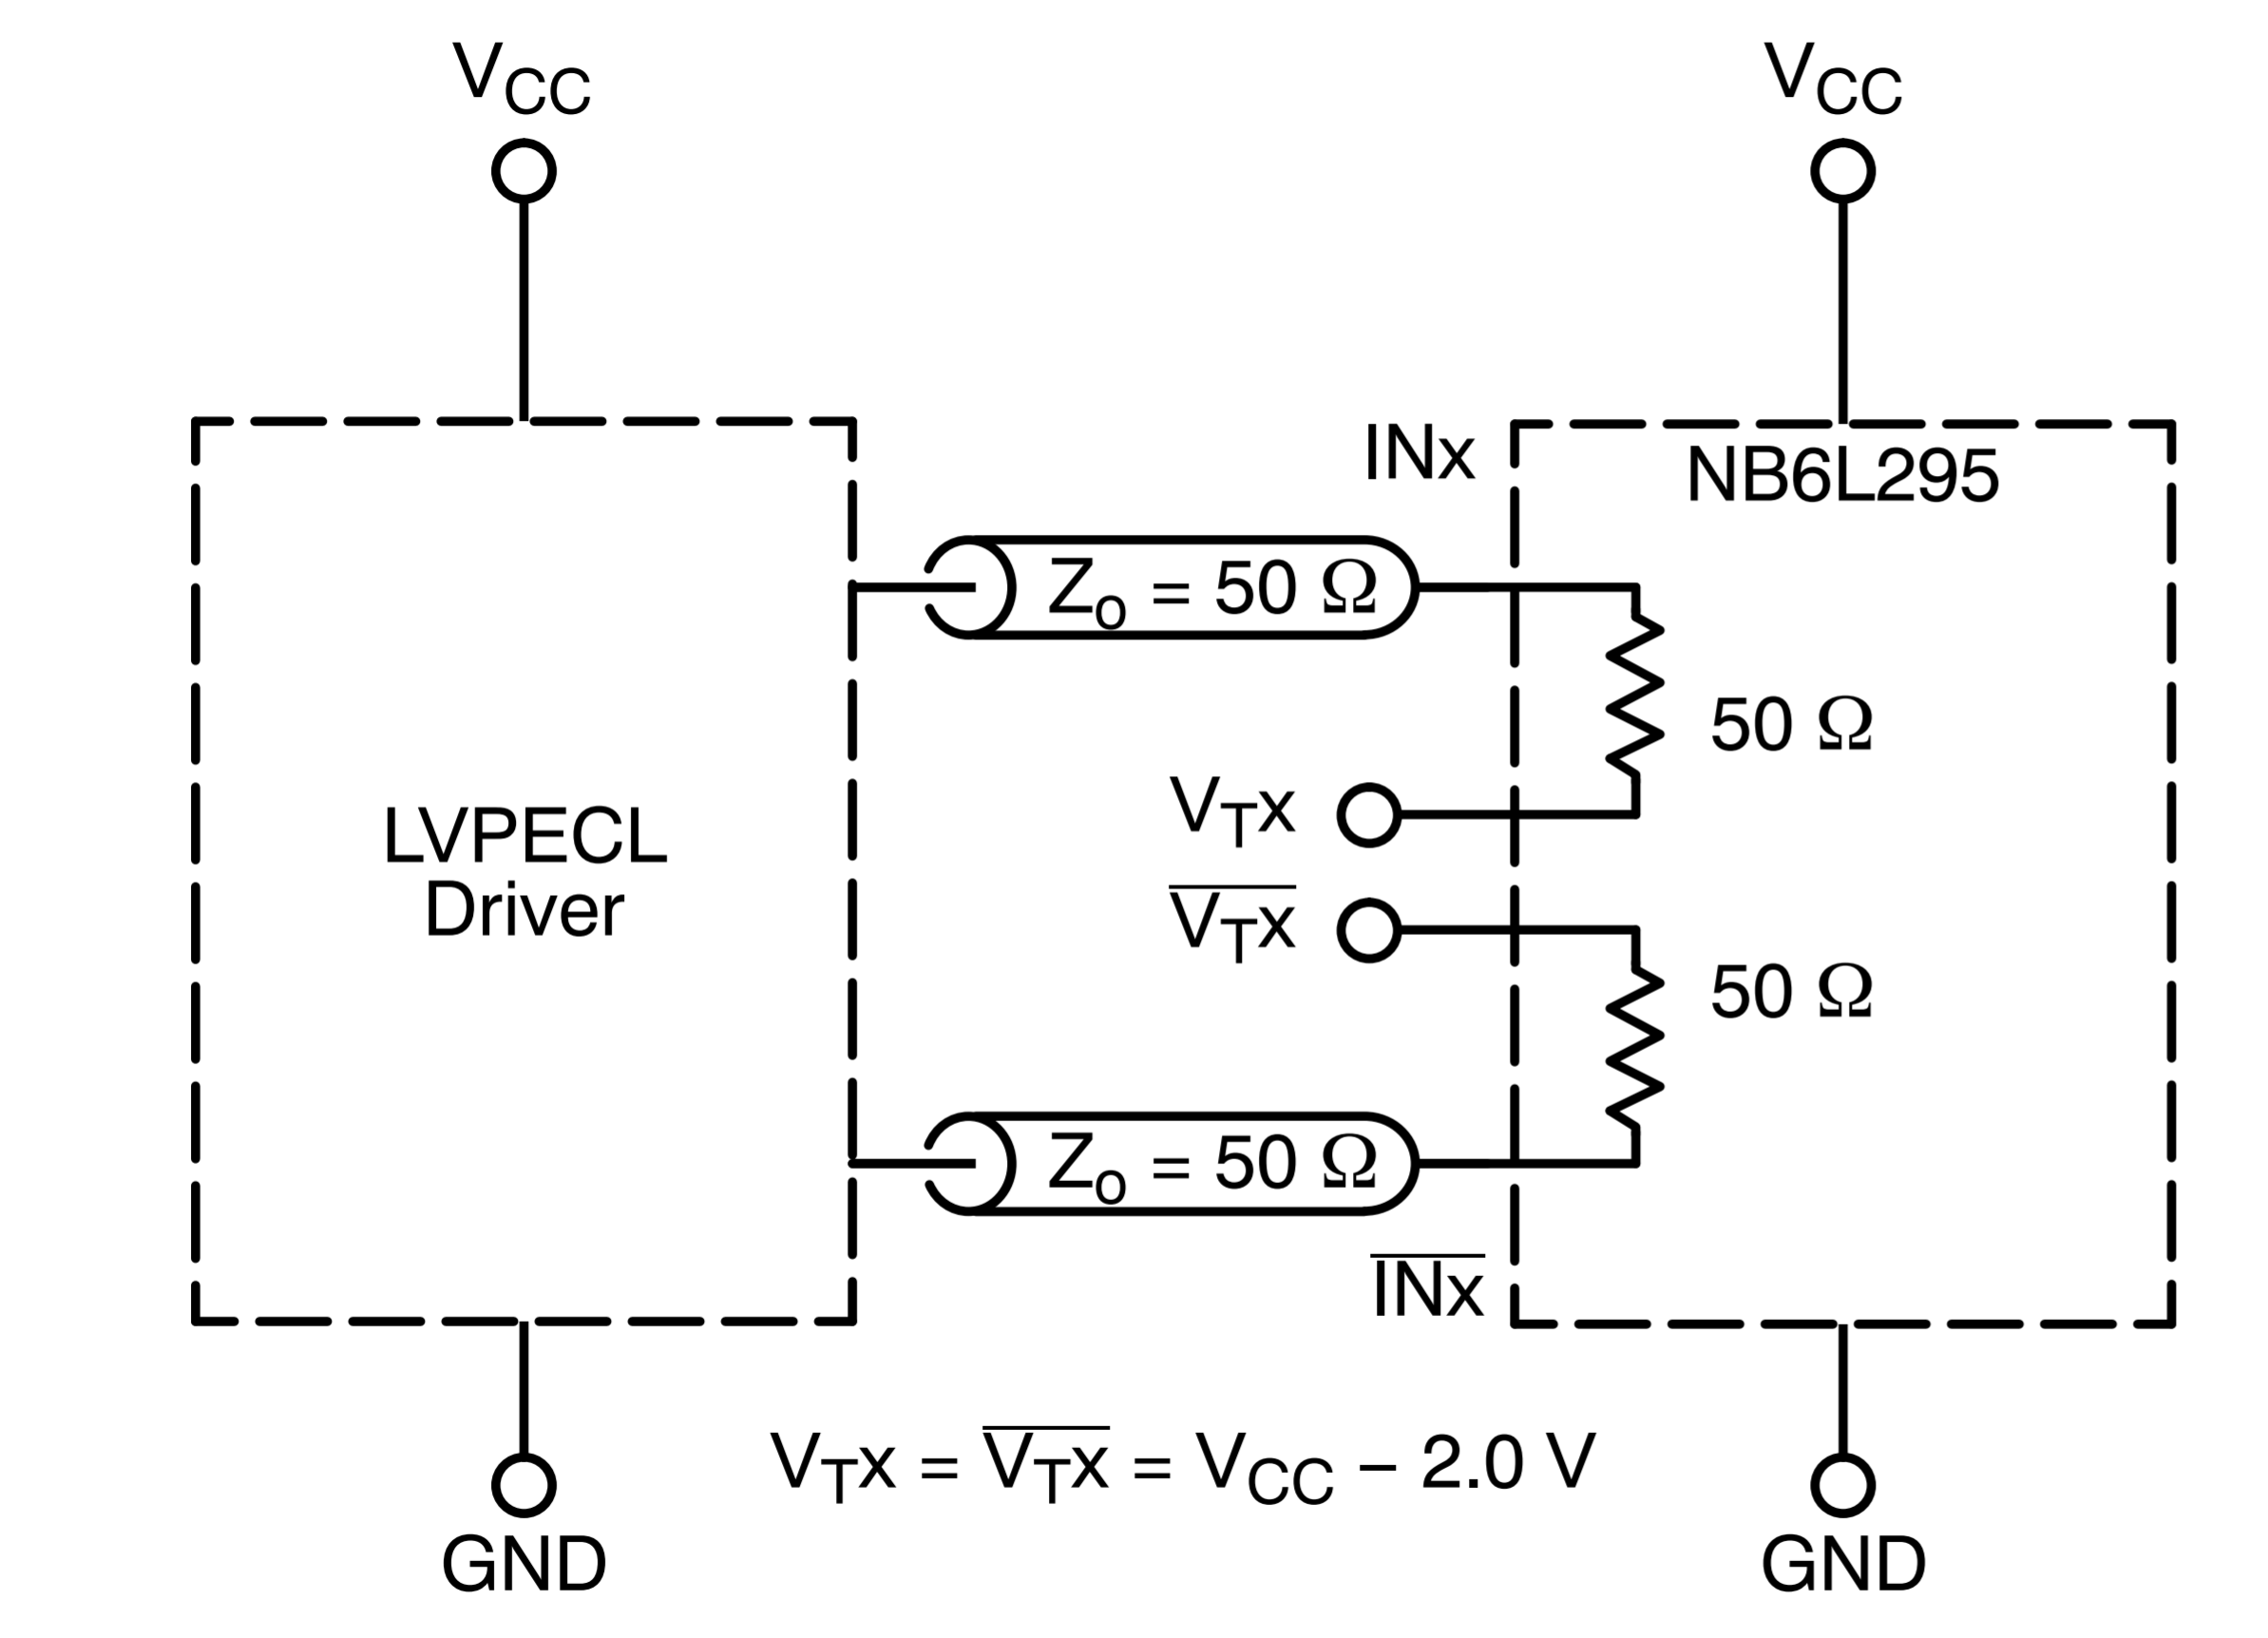
\includegraphics[width = 0.7\textwidth]{chap/04-work/img/delay_lvpecl}
	\caption[NB6L295 Delay Chip Schematic]{LVPECL recommendations for NB6L295 \cite{NB6L295}}
	\label{fig:delay_lvpecl}
\end{figure}


\begin{table}[tbh]
	\caption[NB6L295 Characteristics]{Specifications of the NB6L295 delay chip \cite{NB6L295}}
	\label{tab:nb6l295}
	\begin{minipage}{\textwidth}
		\centering
		\begin{tabularx}{\textwidth}{Xcccc}
			\toprule
			\textbf{Parameter} & \textbf{Min} & \textbf{Typ.} & \textbf{Max} & \textbf{Unit}\\
			\midrule
			\textbf{Outputs} &&&& \\
			Output HIGH Voltage & $V_{cc} - 1075$ & $V_{cc} - 950$ & $V_{cc} - 825$ & mV\\
			Output LOW Voltage & $V_{cc} - 1825$ & $V_{cc} - 1725$ & $V_{cc} - 1625$ & mV\\
			Common mode voltage & -0.1 & 0 & 0.1 & V\\[0.3cm]
			\textbf{AC Characteristics} &&&&\\
			Random Clock Jitter \gls{rms}&  & 3 & 10 & ps\\
			Output Rise/Fall Times (@\SI{50}{\mega \hertz}) & 85 & 120 & 170 & ps\\
			Serial Clock Input Frequency (50\% Duty Cycle\footnote{Percentage of the ratio of pulse width and total period of the waveform.}) &  &  & 20 & MHz\\
			Minimum Pulse width SLOAD  & 1 &  &  & ns\\
			\bottomrule
		\end{tabularx}
	\end{minipage}
\end{table}
%todo fix problem with [XSSSSS]


\subsection{Clocking}
Clocking distribution is designed as shown in \autoref{fig:clocking}. The LMK0480x Low-Noise Clock Jitter Cleaner \gls{pll} from \textit{Texas Instruments} cleans the incoming reference clock coming from the system (e.g. from \gls{kara}) for high temporal accuracy \cite{caselle2013}. It is used with an external \gls{vcxo} from \textit{ABRACON}. The LMK0480x has only 12 outputs, not enough for the 16 \glspl{tha} and additional clocking for \gls{fpga}, \gls{adc} and \gls{dac}, especially considering that the outputs are divided into six groups à two outputs. Outputs in one group have the same configuration (frequency, phase, ...), which means that effectively only six different outputs are available. A low noise clock distribution fanout buffer, the HMC987LP5E from \textit{Analog Devices} is therefore used for distributing the clock signal to the delay chips. As one fanout buffer has eight outputs, two chips are needed to cover all channels. One output of the \gls{pll} is propagated to the \gls{fmc}+ connector as reference clock for the \gls{fpga}. Up until this part, this architecture is not different from the one on the \gls{kapture} sampling board. 

\begin{figure}[tbh]
	\centering
	\includegraphics[width = \textwidth]{chap/04-work/img/pll_tsMode}
	\caption{Placeholder}
	\label{fig:clocking}
\end{figure}
%todo clean picture

The maximum output frequency of the LMK0480 is \SI{1536}{\mega \hertz}, not enough to clock the \glspl{adc} at maximum sampling rate (\SI{2.5}{\giga \sample \per \second}). A second \gls{pll} is therefore needed. The read-out card is provided with an \gls{rf} Clock add-on card, which is necessary to generate the high-frequency clocks for the converters. The LMX2594 from \textit{Texas Instruments} provides clocking signal up to \SI{15}{\giga \hertz} and is a fitting candidate. For loop filter calculation, the TI PLLAtinum Sim Tool is used. The parameters for the filter are as shown in \autoref{tab:lmx2594_filter}.

\textbf{TODO} 
\begin{itemize}
	\item Needs some more explanation and maybe at least a little bit theory (e.g. block diagram of general PLL and what loop filter is)
	\item Maybe some simulation diagram with the PLLatinum Tool (used for calculation of the noise, jitter, etc. over the frequency)
\end{itemize}

\begin{figure}[tbh]
	\centering
	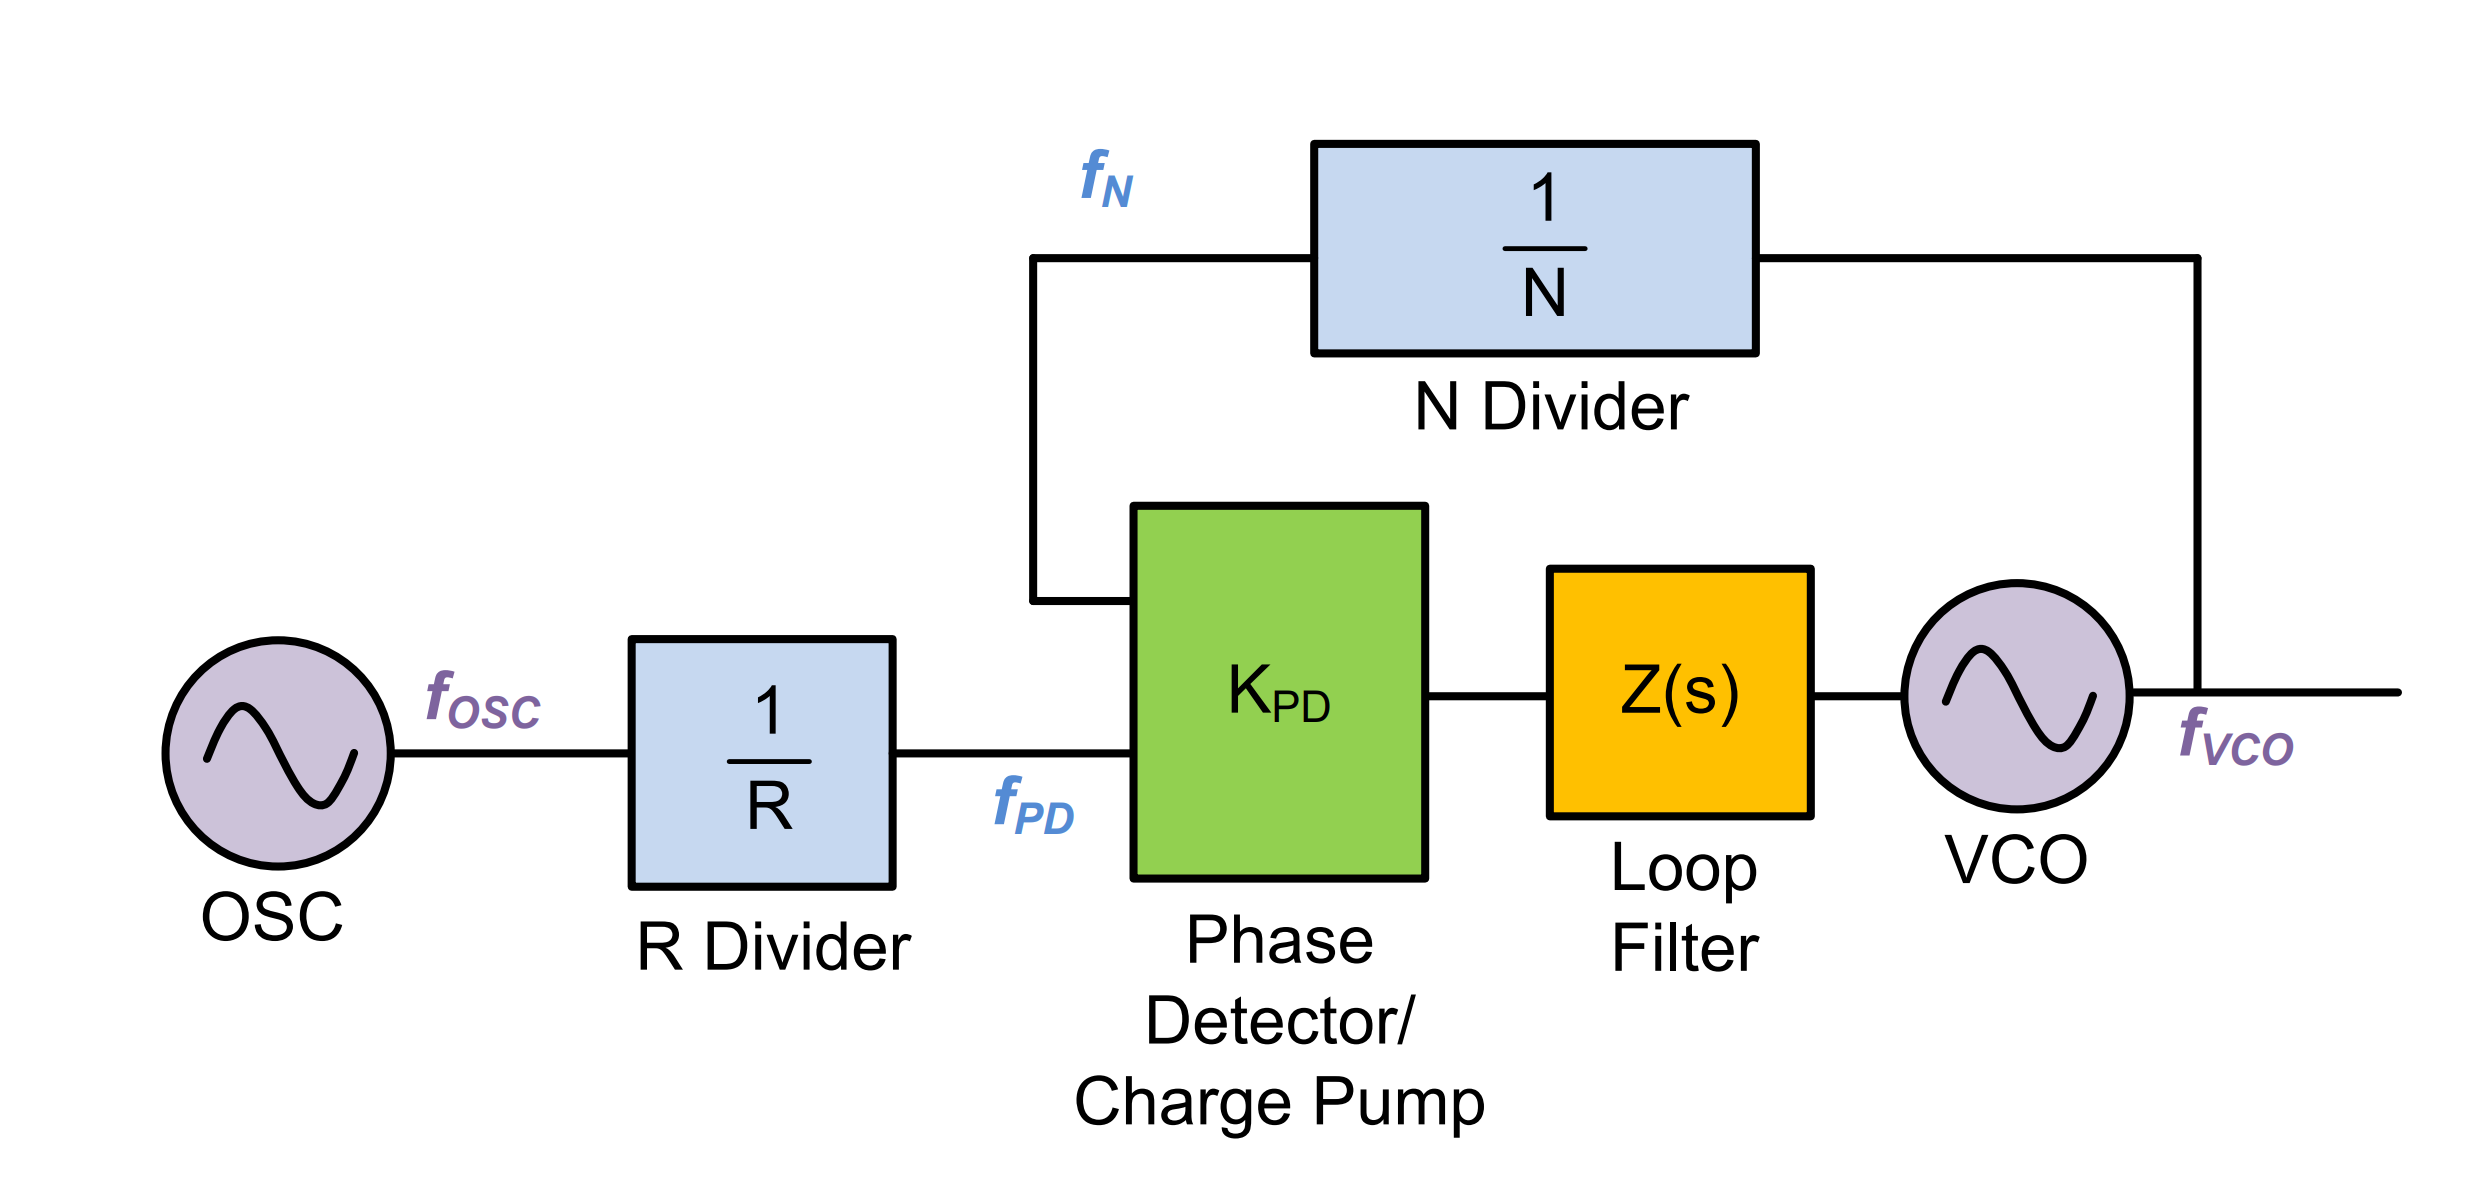
\includegraphics[width = \textwidth]{chap/04-work/img/pll_block}
	\caption[PLL block diagram]{General block diagram of a \gls{pll}}
	\label{fig:pll_block}
\end{figure}


\begin{table}[tbh]
	\caption[LMX2594 Filter characteristics]{Filter characteristics}
	\label{tab:lmx2594_filter}
	\centering
	\begin{tabularx}{\textwidth}{Xl}
		\toprule
		\textbf{Parameter} & \textbf{Value} \\
		\bottomrule
		 VCO Gain & \SI{239}{\mega \hertz \per \volt} \\
		 Loop Bandwidth	 & \SI{32.7}{\kilo \hertz} \\
		 Phase Margin	 & 69 deg \\
		 Effective Charge Pump Gain	 & \SI{3}{\milli \ampere} \\
		 Phase Detector Frequency & \SI{24.576}{\mega \hertz}\\
		 VCXO Frequency	& Designed for \SI{15}{\giga \hertz} (works for all)\\ [0.3cm]
		 \textbf{Loop filter components} & \\
		 $C_{1,LF}$ &  \SI{2200}{\pico \farad}\\
		 $C_{2,LF}$ &  \SI{180}{\nano \farad}\\
		 $C_{3,LF}$ &  \SI{1800}{\pico \farad}\\
		 $R_{2}$ &  \SI{160}{\ohm}\\
		 $R_{3,LF}$ &  \SI{180}{\ohm}\\
		 \bottomrule
	\end{tabularx}
\end{table}

%todo deg

\begin{figure}[tbh]
	\centering
	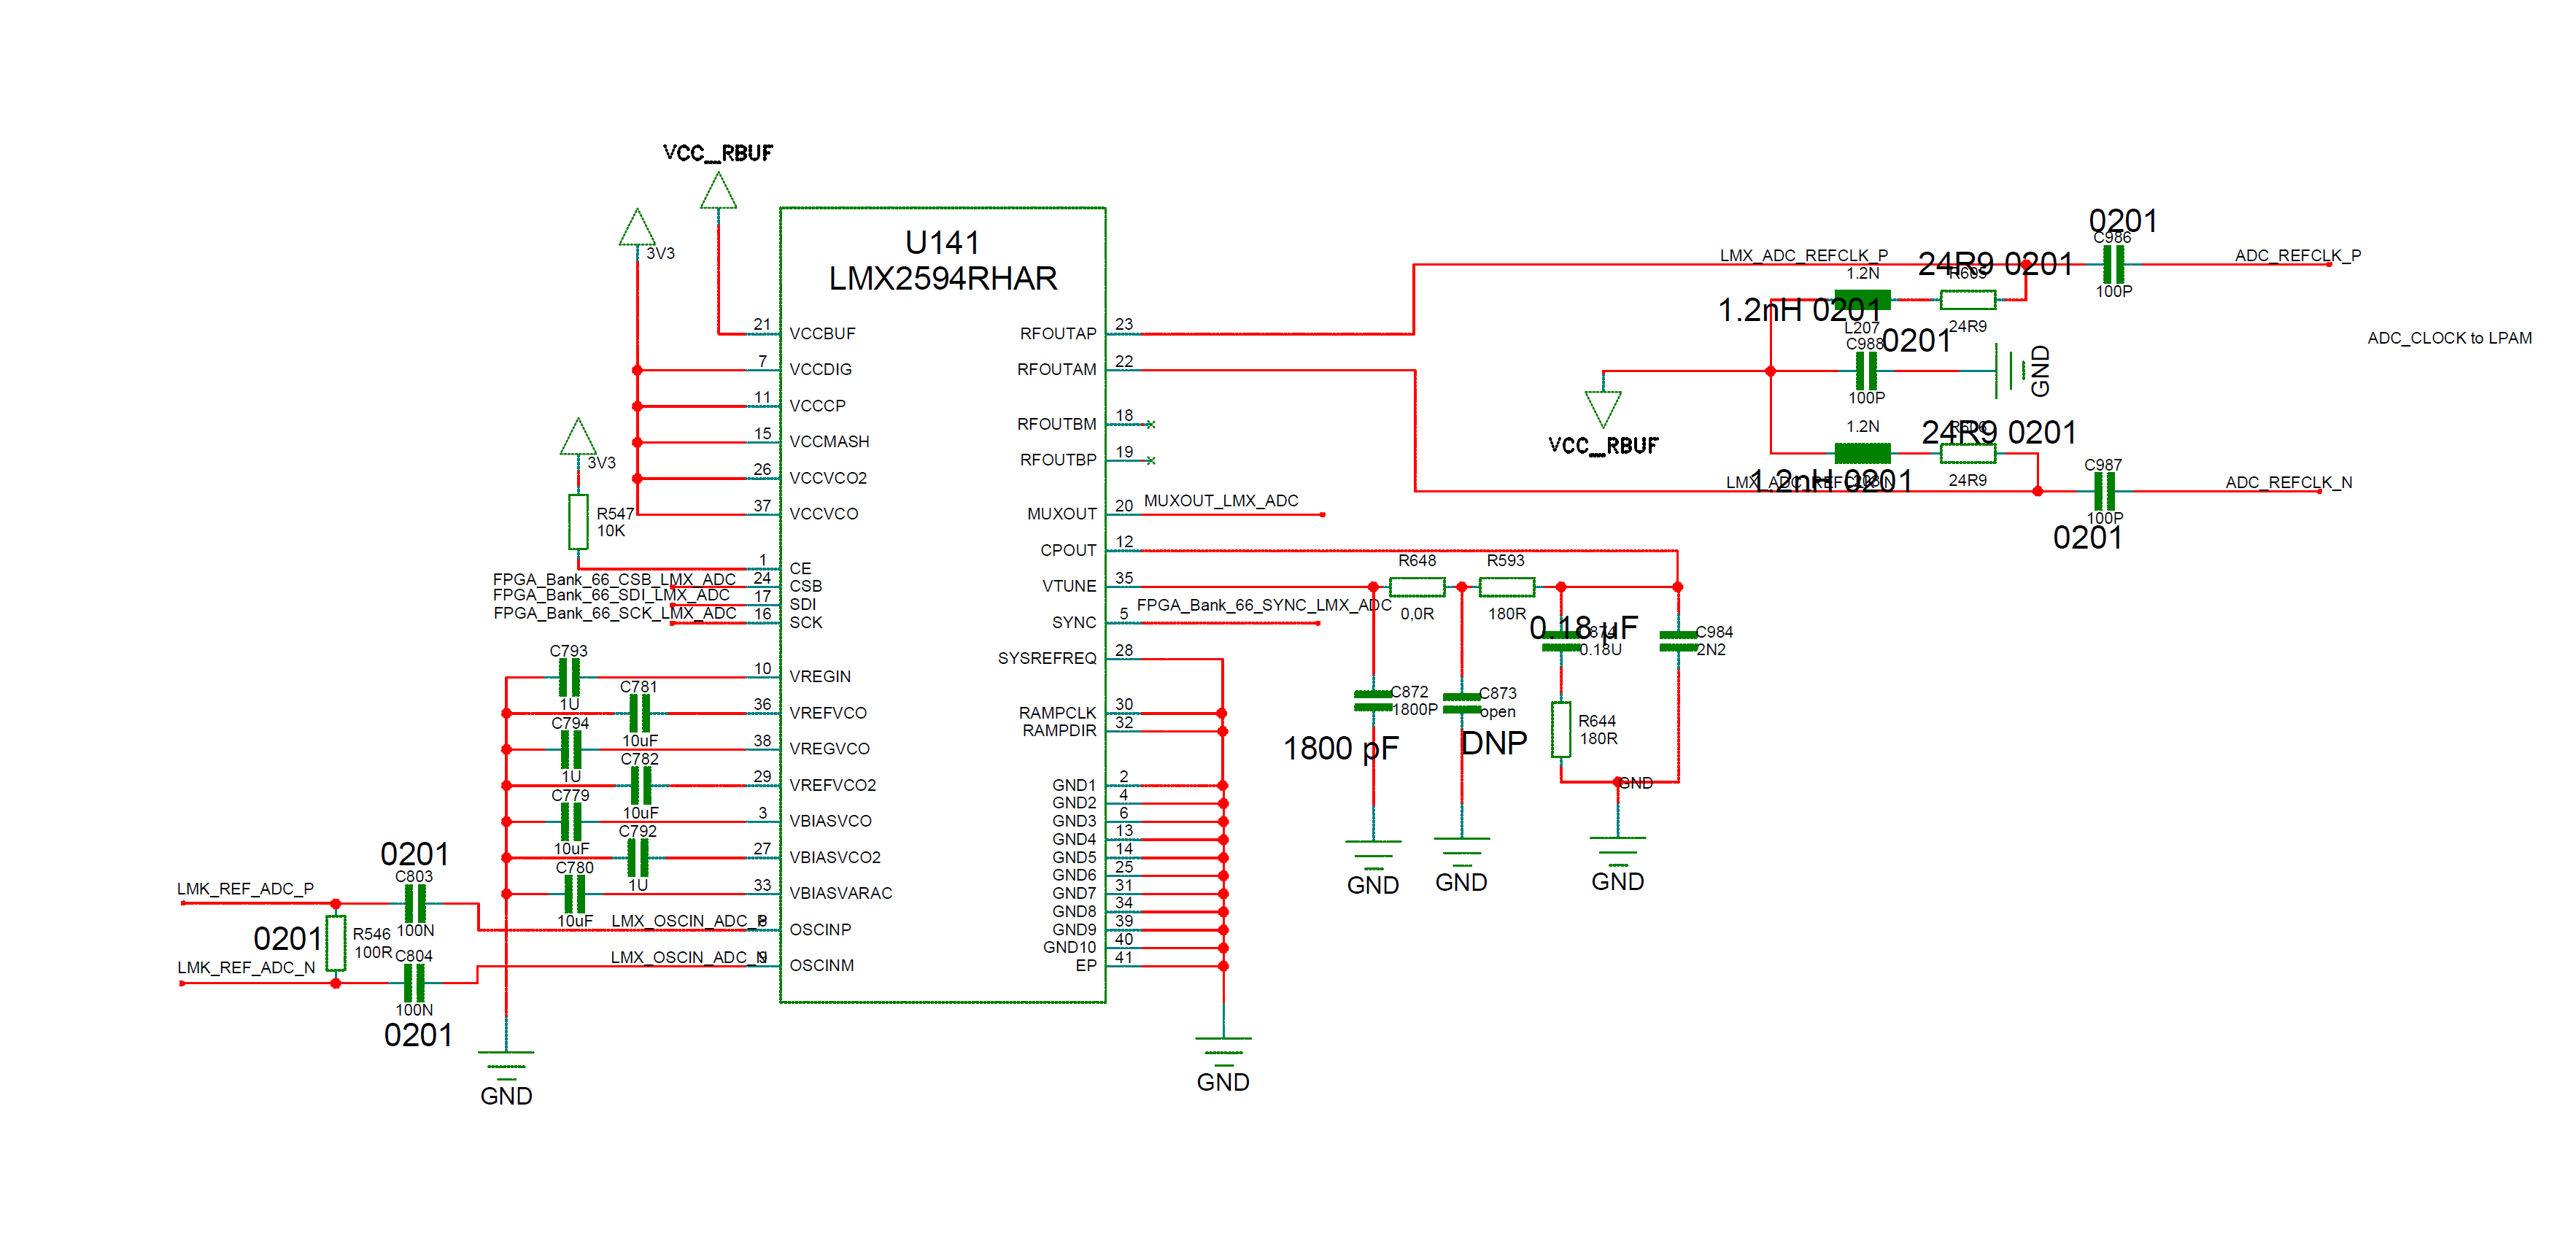
\includegraphics[width = \textwidth]{chap/04-work/img/lmx2594}
	\caption{Schematics of the LMX2594}
	\label{fig:lmx2594}
\end{figure}

\textbf{TODO}: Explain with help of timing diagram, why ADCs need to be at different PLLs -> outputs not individually programmable. phase difference between clocks needs to be 180° -> like two times interleaving

The necessary step size for the delay chips, when using 16 ADC@\SI{2}{\giga \sample \per \second} in time-interleaving mode, is: $\frac{\SI{2}{\giga \sample \per \second}}{16} = \SI{31}{\pico \second}$
However, providing individual clocks to the ADCs is not possible on the ZCU216 card. ADCs are grouped together into tiles, each tile containing four converters. One single reference clock signal is propagated to all tiles. Sampling clock is adjusted at each tile individually, however this clocking signal is the same for all of the four converters in the tile. Normally, only one reference clock can be provided. Analyzing the schematic of the zcu216 board revealed however, that there are pins leading to the FPGA banks (224 to 227), labeled as clocks for the individual tiles. Two of the clocks are not connected (224 and 227). 225 is provided via SMA cable, the other comes from the LPAM clock connector.  

Clock to THA: \SI{500}{\mega \hertz}

Total Hold time: \SI{1}{\nano \second}

$\rightarrow$ Step size for delay:
\begin{equation}
	\frac{\SI{1}{\nano \second}}{16 \, \text{channels}} = \SI{62.5}{\pico \second}
\end{equation}

Aperture delay, jitter, need to be taken into account to determine the max. sampling frequency.
\begin{figure}[tbh]
	\centering
	\tikzexternaldisable
	\begin{tikztimingtable}
		TH1 & 1L 8H N(A1) 8H 16L \\
		TH2 & 2L 16H 15L \\
		TH3 & 3L 16H 14L \\
		TH4 & 4L 5H N(B1) 11H 13L \\
		\\
		TH5 & 5L 8H N(A2) 8H 12L \\
		TH6 & 6L 16H 11L \\
		TH7 & 7L 16H 10L \\
		TH8 & 8L 5H N(B2) 11H 9L \\
		\\
		TH9 & 9L 8H N(A3) 8H 8L \\
		TH10 & 10L 16H 7L \\
		TH11 & 11L 16H 6L \\
		TH12 & 12L 5H N(B3) 11H 5L \\
		\\
		TH13 & 13L 8H N(A4) 8H 4L \\
		TH14 & 14L 16H 3L \\
		TH15 & 15L 16H 2L \\
		TH16 & 16L 5H N(B4) 11H 1L \\
		\extracode
		\tablerules
		\draw [dashed] (A1) --node[midway, anchor = west]{ADC1} (B1) ;
		\draw [dashed] (A2) --node[midway, anchor = west]{ADC2} (B2) ;
		\draw [dashed] (A3) --node[midway, anchor = west]{ADC1} (B3) ;
		\draw [dashed] (A4) --node[midway, anchor = west]{ADC2} (B4) ;
	\end{tikztimingtable}
	\tikzexternalenable
	\caption[Track-And-Hold Timing diagram]{\gls{tha} Timing diagram. Shows the clocking of the \gls{tha}, high level = HOLD, low level = TRACK. Dashed line represents the sampling of the \gls{adc}.}
	\label{fig:THA}
\end{figure}
%todo what does the dashed line show?


\subsection{Digital-To-Analog-Converter Balun Channel}
For test purposes, two \gls{dac} channels from the read-out card are routed on the sampling board. In this way, test signals can be generated right on the read-out card, without the need for an external signal generator. 

\begin{figure}[tbh]
	\centering
	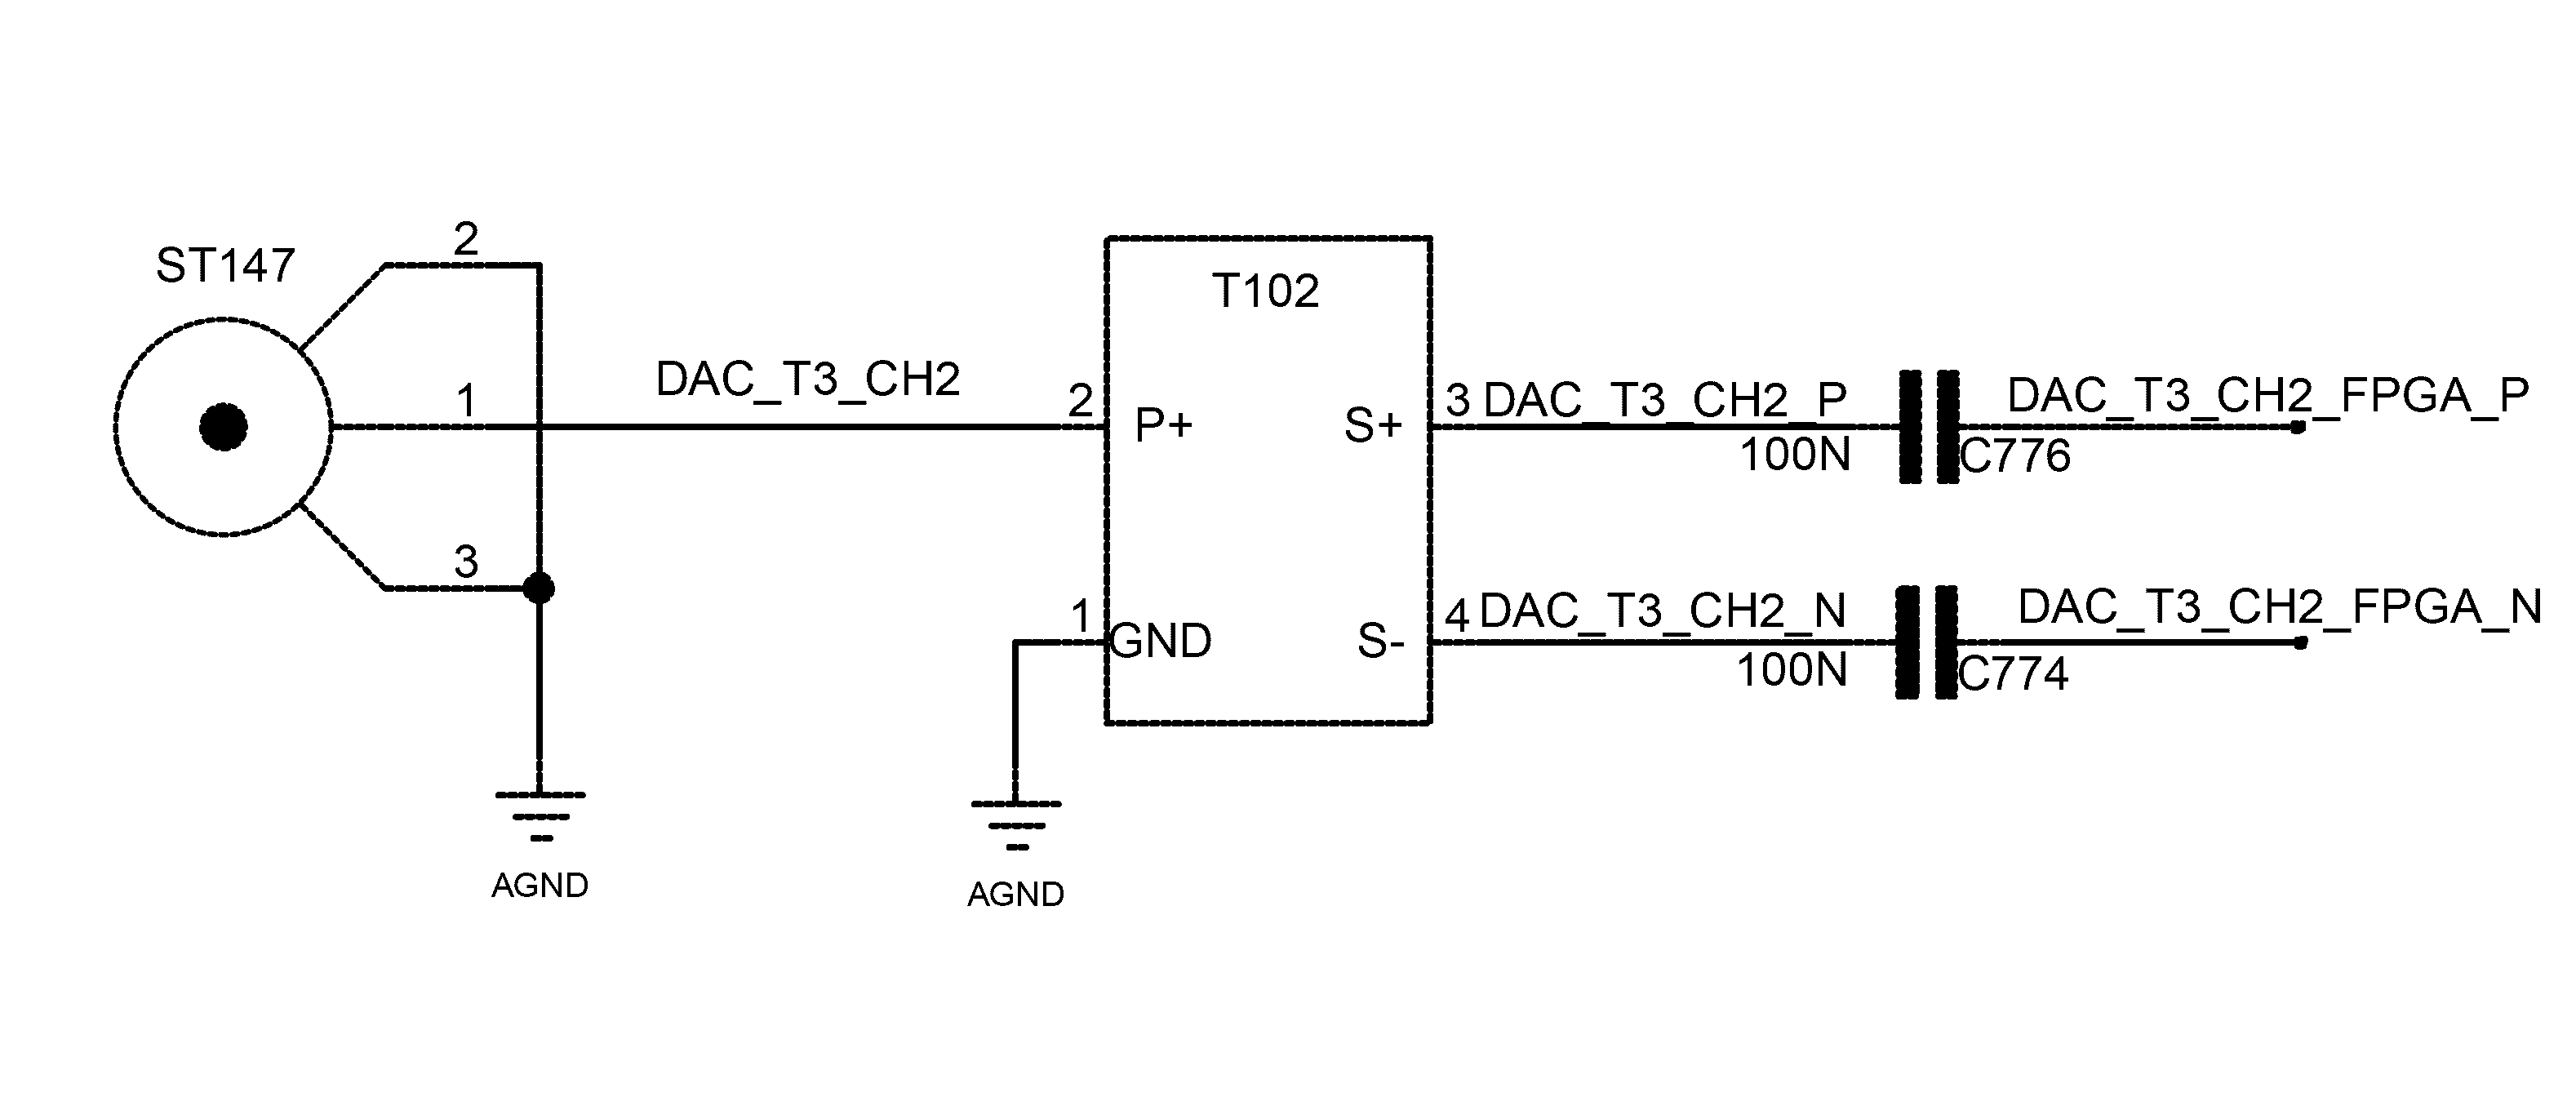
\includegraphics[width = \textwidth]{chap/04-work/img/dac_channel}
	\caption{DAC-channel with balun. Signal travels from right to left.}
	\label{fig:dac_channel}
\end{figure}


\subsection{Power Supply}
On the \gls{kapture} sampling board, the ADP1708 from \textit{Analog Devices} is used to provide a power supply for the \glspl{tha}. 
For the Track-And-Hold amplifiers on the new board, another power supply unit, the ADP1741 from \textit{Analog Devices}, should be used. This power supply can handle more maximum current, therefore less power supplies are needed. This is important considering the higher number of components. 

It is necessary to think about the amount of power supply chips needed. As a rule of thumb, the power supply should provide twice the maximum power needed by the components it drives. \cite{michele} The power consumption/maximum current for the respective components on the sampling board is listed in \autoref{tab:kapturecomp}. 
\begin{table}[tbh]
	\caption{Power consumption of components on the board}
	\label{tab:kapturecomp}
	\begin{minipage}{\textwidth}
		\centering
		\begin{tabularx}{\textwidth}{Xlllll}
			\toprule
			\textbf{Component} & $V_{cc}$ (V) & $I_{max}$ (A) & $P_{max}$ (W) & $\#_{parts}$ &  $I_{tot}$\footnote{for 16 \glspl{adc}} (A)  \\
			\midrule
			HMC5649 \gls{tha} 	& 2	  	& 0.221 	 & 0.442 & 16 & 3.536\\
			& -5  	& -0.242 & 1.21 &  & 3.872\\
			HMC856 (Delay) 			& -3.3	& 0.185 & -0.611 & 16 & 2.96\\
			HMC987LP5E (Fan-Out buffer) 	& 3.3 	& 0.234\footnote{All Outputs and RF-Buffer} & 0.772 & 2 & 0.468\\
			LMC0480 \gls{pll}			& 3.3 	& 0.590\footnote{All CLKs} & 1.947 & 1 & 0.590\\
			VCXO 					& 3.3 	& 0.03 & 0.198 & 1 & 0.03\\
			
			\bottomrule
	\end{tabularx}
	\end{minipage}
\end{table}

The maximal current which the ADP1741 can provide @\SI{2}{\volt} is \SI{2}{\ampere}. This means, with one Track-And-Hold amplifier requiring a maximal current of \SI{0.221}{\ampere}, one ADP1741 can handle four units according to the rule mentioned beforehand ($I_{max\_ADP1741} = \SI{2}{\ampere} > 2 * I_{tot}, I_{tot} = 4 \times \SI{0.221}{\ampere} =  \SI{0.884}{\ampere}$).



\section{Layout}
%Both analog and digital signals require a wideband
%signal propagation and a low noise of both voltage and
%time levels. Therefore the PCB is made by ROGER 4003
%material and the signals are routed by dedicated
%transmission lines. Well separated analog and digital
%grounds in conjunction with ad-hoc RF filters located
%closer at the critical components have been adopted to
%reduce the influence of the digital circuit on the analog
%devices. Moreover, the via fences and guard ring
%techniques have been employed in the PCB layout in
%order to reduce the cross-talk between adjacent
%transmission lines, the electromagnetic interference (EMI)
%and improve the performance at high frequency [6]. A low
%time jitter is required, which is dependent on deterministic
%and Gaussian contributions. The deterministic jitter (DJ)
%depends on the duty cycle distortion, cross-talk, EMI, etc.
%This component has been drastically reduced by the
%techniques mentioned before regarding hardware layout
%techniques, moreover, the residual noise can be measured
%and corrected in the FPGA.


\subsection{PCB Structures Overview} \label{ssec:pcb_structs}
An overview over the basic structures on a \gls{pcb} is given.

\paragraph{Traces}
A \textit{trace} is a strip of metal, which establishes an electrical connection and carries signals between two (or more) points in the horizontal plane of a \gls{pcb}. \cite{xilDecouple}


\paragraph{Planes}
\textit{Plane} denotes an uninterrupted area of metal, which covers the whole \gls{pcb} layer. If this area only covers only part of the layer, it is called a \textit{planelet}. These areas provide power distribution across the \gls{pcb} and present an important transmission medium for the return current\footnote{Any current, which is injected into the components/boards, needs a return path, as otherwise there is no closed circuit.}. \cite{xilDecouple}

\paragraph{Vias}
A via is metal-plated hole, which is used to route a trace in vertical direction, i.e. from the \gls{pcb} outer layer to the inner layers. They carry signals and power. Three types of vias are \cite{vias}:
\begin{itemize}
	\item Blind via: A blind via connects the surface layers with at most three layers below.
	\item Buried via: A buried via only connects internal layers.
	\item Through via: A through via goes from one \gls{pcb} surface to another and is used to connect any layer. 
\end{itemize}
\begin{figure}[tbh]
	\centering
	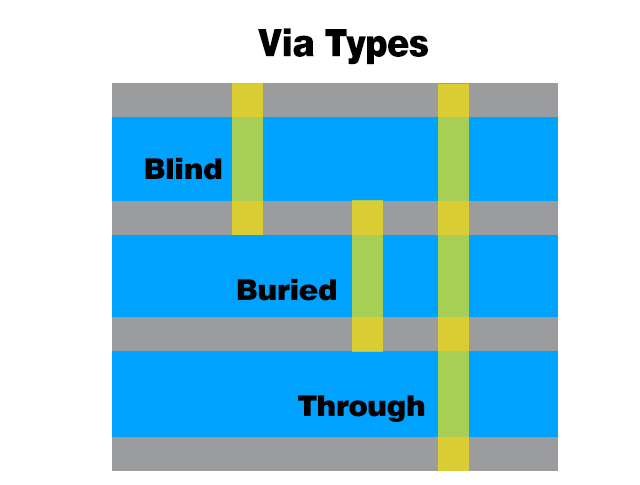
\includegraphics[width = 0.7\textwidth]{chap/04-work/img/vias}
	\caption[Via types]{Visualization of via types \cite{vias}}
	\label{fig:vias}
\end{figure}

\textbf{TODO:} 
	\begin{itemize}
		\item Via fences
		\item Pads
	\end{itemize}
%todo bild

In this design only blind and through vias are used.

\subsection{\gls{pcb} Substrate}
TODO
Megtron6 Laminate R-5775 Prepreg R-5670

$\epsilon_r = 3.61$ at \SI{10}{\giga \hertz}, $\epsilon_r = 3.71$ at \SI{1}{\giga \hertz}
\subsection{Floor Planning}
TODO
\subsection{Transmission lines}

Transmission lines carry high-frequency signals, therefore the geometry of them is important, as this affects the impedance. For single-ended the waveguide characteristic impedance should be \SI{50}{\ohm}, for differential signals \SI{100}{\ohm}. For slow signals not that crucial, but for sensitive, high-speed signals, e.g. clocking signals, proper calculation is very important to ensure signal integrity and reduce reflection and damping. 

For \glspl{pcb} usually coplanar waveguides are used for signal propagation. The characteristic impedance depends on the dielectric, the trace width, separation between traces and separation between the signal traces and the ground planes/traces. Formulas to calculate the characteristic impedance are quite lengthy and not easy to solve. Luckily, tools\footnote{which are quite expensive though, if a high variety of geometries is necessary} exist to quickly calculate the geometric values needed for appropriate impedance. For the design, the Si9000e \gls{pcb} field solver from \textit{Polar} (see \autoref{fig:polaris})is used to calculate the necessary trace widths, separations, etc.

\begin{figure}[tbh]
	\centering
	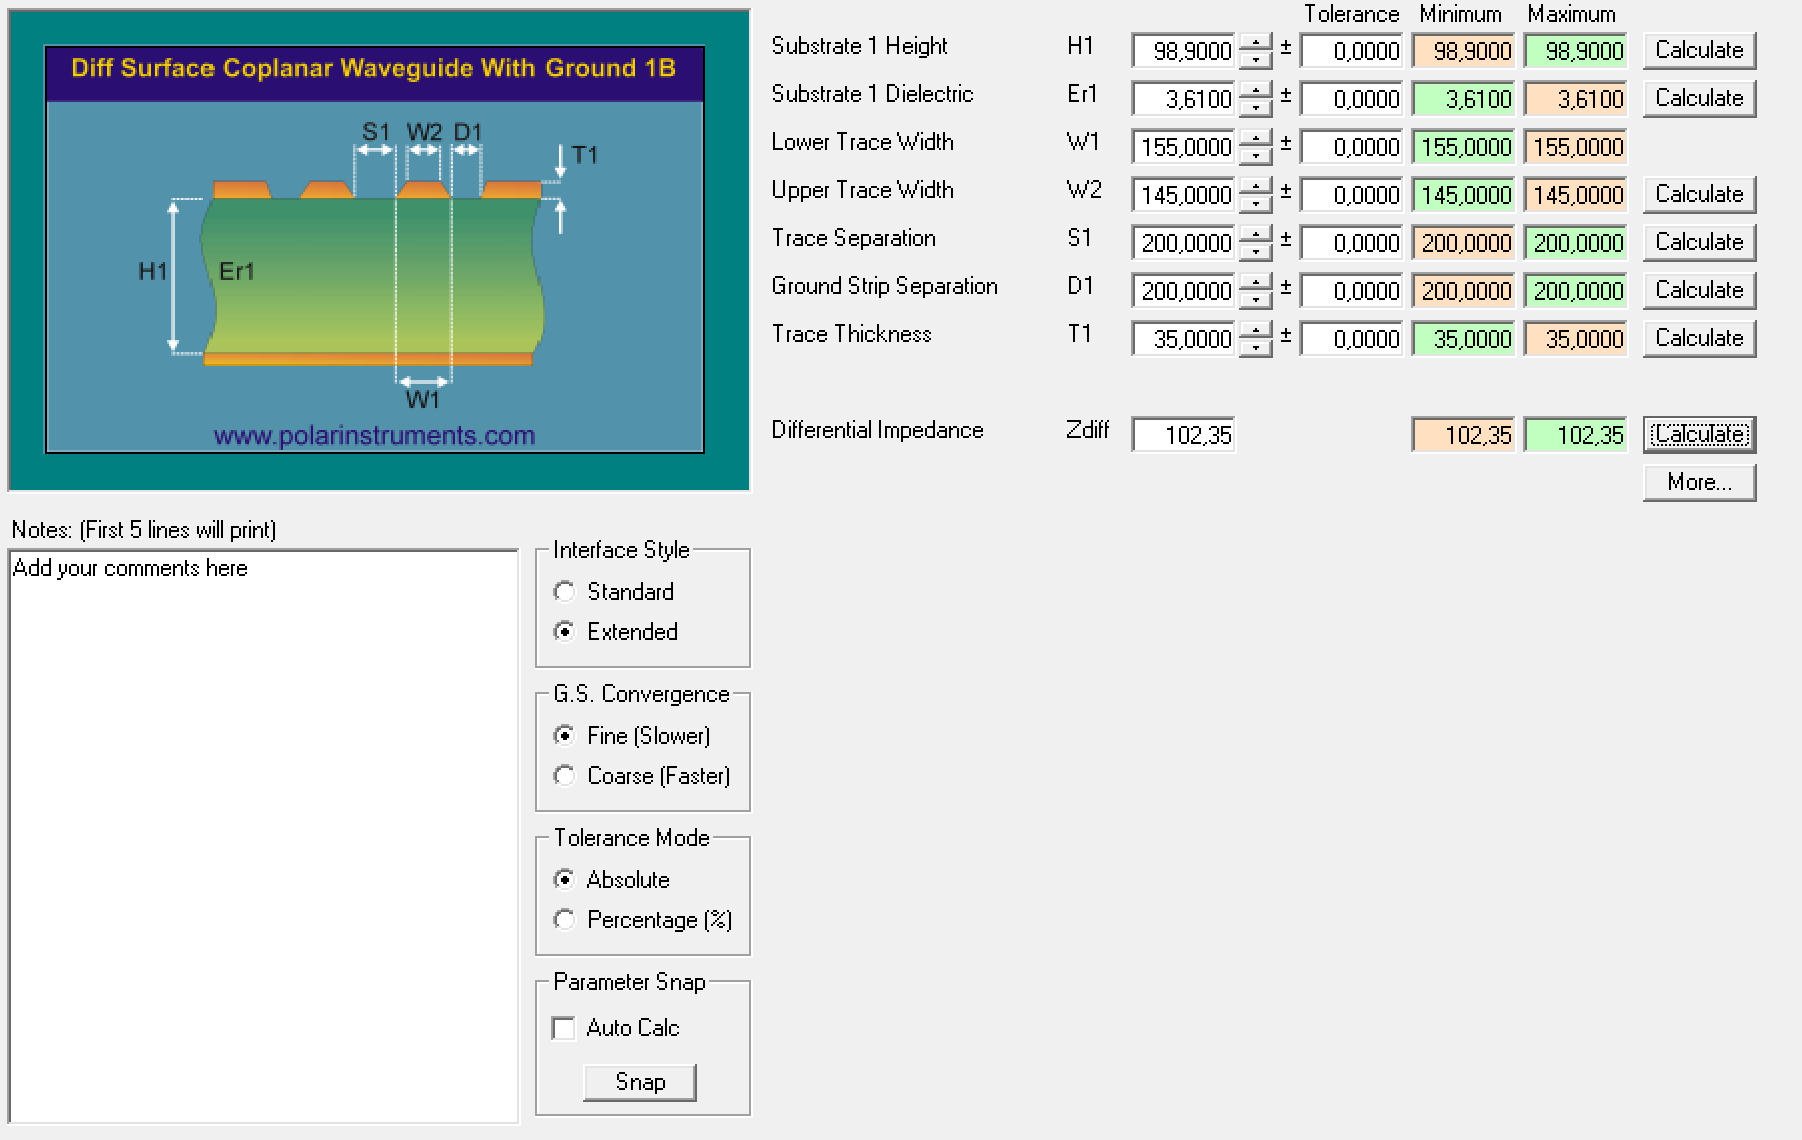
\includegraphics[width = \textwidth]{chap/04-work/img/polaris}
	\caption{Polaris Solver}
	\label{fig:polaris}
\end{figure}

Three geometries of waveguides are used in this design which are described in the following. Furthermore, geometric dimensions calculated with the Si9000e tool are presented. In principle, the geometries can be taken from the design of the sampling card of \gls{kapture} system. As the dielectric constant of the substrate is slightly different (\gls{kapture}: 3.52, here: 3.61), the impedance has to be recalculated to check whether the characteristic value impedance still lies in the 10\% tolerance.
\paragraph{Surface Coplanar Waveguide with Ground}
The surface coplanar waveguide has the geometry shown in \autoref{fig:microstrip_geometry}. The single trace of the thickness $t$ and width $a$ lies between two ground planes on a dielectric of thickness $h$ and the effective dielectric constant $\epsilon_r$. Another ground plane is located at the bottom of the dielectric. Separation between trace and ground plane is calculated as $(b-a)/2 := d$. 

\begin{figure}[!htbp]
	\centering
	\includegraphics[width = \textwidth]{chap/04-work/img/cw}
	\caption{Coplanar Waveguide with Ground}
	\label{fig:microstrip_geometry}
\end{figure}

Trace width is assumed to be $a = \SI{180}{\micro \meter}$. In the tool, an upper and a lower trace width can be specified, therefore taking into account manufacturing processes. As the exact upper trace width is not known, both are assumed to be  \SI{180}{\micro \meter}.   Trace-To-Ground Separation, or "Ground Strip Separation", is defined by the manufacturing technology of the \gls{pcb} process: $d = \SI{250}{\micro \meter}$ With $h = \SI{98.9}{\micro \meter}$, $\epsilon_r = 3.61$ (at \SI{10}{\giga \hertz}) this results in a characteristic impedance of \SI{52.90}{\ohm}. This lies well in the tolerance area.

To study the effect of changing parameters, some calculations were done with the tool (it provides possibility to plot Zo vs. parameter or parameter vs. parameter with fixed Zo).
Over the frequency range, the value of the effective dielectric constant changes from 3.71 (at \SI{1}{\giga \hertz}) to 3.61 (at \SI{10}{\giga \hertz}). As the tool provides the possibility to calculate the impedance versus a changing parameter, the influence of a changing dielectric was calculated. As can be seen in \autoref{fig:surf_z0_vs_dk}, with higher effective dielectric constant, the characteristic impedance decreases (see \autoref{fig:surf_z0_vs_dk}).

The only parameters, which are not defined by the manufacturing process and therefore can be altered, are the ground strip separation and the trace width. When altering the trace width, the tool automatically assumes an upper trace width, which is \SI{25}{\micro \meter} smaller than the lower trace width. Therefore plot can provide qualitative behavior, but not exact for the design at hand.

\textbf{TODO}: fix plot. too big

\begin{figure}
	\centering
	\includegraphics[width = \textwidth]{chap/04-work/img/surf_z0_vs_dk.tikz}  
	\caption{Characteristic impedance $Z_o$ vs effective dielectric constant $\epsilon_r$ of a surface coplanar waveguide with ground}
	\label{fig:surf_z0_vs_dk}
\end{figure}

%\begin{figure}
%		\centering
%		\includegraphics[width = \textwidth]{chap/04-work/img/surf_z0_vs_d1.tikz}
%		\caption{Characteristic impedance $Z_o$ vs effective dielectric constant $\epsilon_r$ of a surface coplanar waveguide with ground}
%		\label{fig:surf_z0_vs_d1}
%\end{figure}


 \paragraph{Differential Pairs on Surface}
\begin{figure}[!htbp]
	\centering
	\includegraphics[width = \textwidth]{chap/04-work/img/eccw}
	\caption{Edge-Coupled Coplanar Waveguide}
	\label{fig:eccw_geometry}
\end{figure}

\paragraph{Differential Pairs between Layers}
\begin{figure}[!htbp]
	\centering
	\includegraphics[width = \textwidth]{chap/04-work/img/docw}
	\caption{Differential Offset Coplanar Waveguide}
	\label{fig:docw}
\end{figure}






\section{Production}
   	\chapter{Back-End Readout Card and System Integration}\label{chap:readout}
   			The back-end readout card for the system under development, the Zynq UltraScale+ RFSoC ZCU216 Evaluation Card, was chosen taking into consideration the points described in \autoref{sec:selection}.
In this section, the overall architecture and features of the card are presented.
A possibility for evaluation of the card is also demonstrated.
At last, a design for the read-out firmware is proposed. 

\section{Xilinx Zynq UltraScale+ RFSoC ZCU216 Evaluation Card}
Zynq UltraScale+ RFSoCs: Combine RF data converter subsystem and forward error correction with industry-leading
programmable logic and heterogeneous processing capability. Integrated RF-ADCs, RF-DACs, and soft decision FECs (SD-FEC)
provide the key subsystems for multiband, multi-mode cellular radios and cable infrastructure


With the data converters integrated directly into the \gls{fpga} using parallel interfaces, they do not require the
prohibitively high-pin-count external connections needed for discrete parallel interface converters, allowing more converter

\begin{itemize}[noitemsep]
	\item Sixteen 14-bit, 2.5GSPS RF-ADC
	\item Sixteen 14-bit, 10GSPS RF-DAC
	\item I/O expansion options – FPGA Mezzanine Card (FMC+) interfaces, RFMC 2.0 interfaces, and Pmod connections
\end{itemize}
\begin{figure}[tbh]
	\centering
	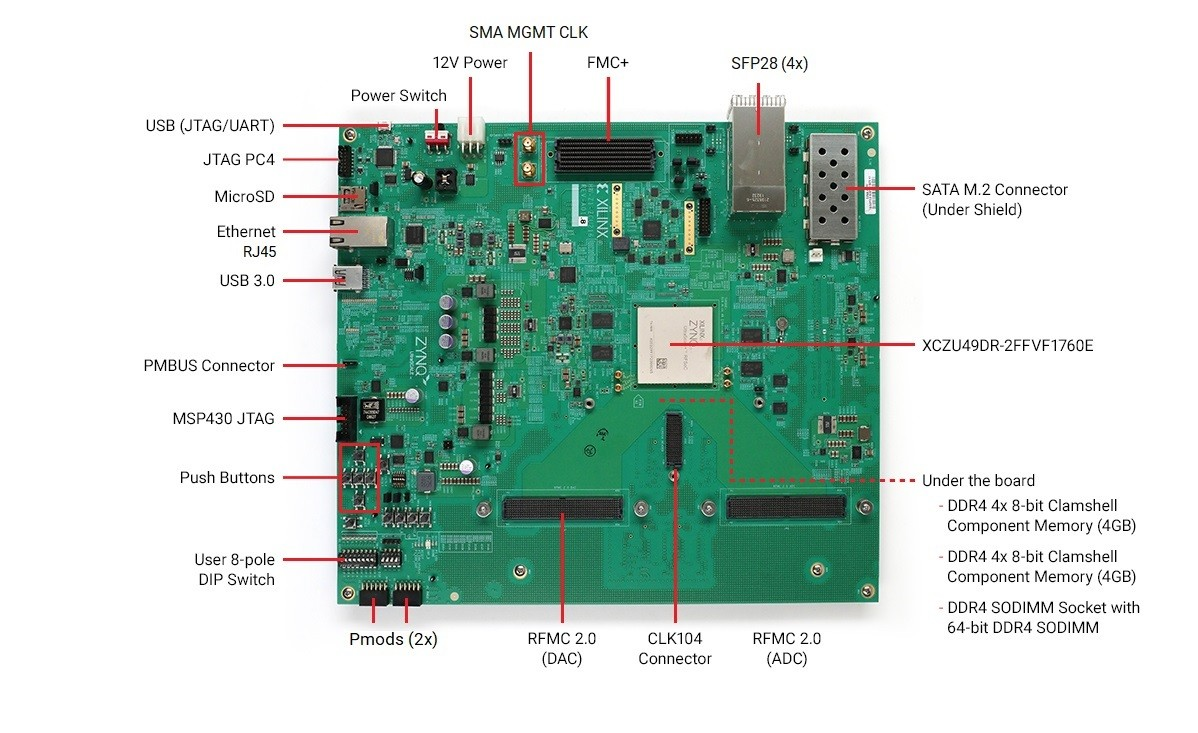
\includegraphics[width = \textwidth]{chap/04-work/img/zcu216}
	\caption{ZCU216 evaluation board}
	\label{fig:zcu216}
\end{figure}

\begin{figure}[tbh]
	\centering
	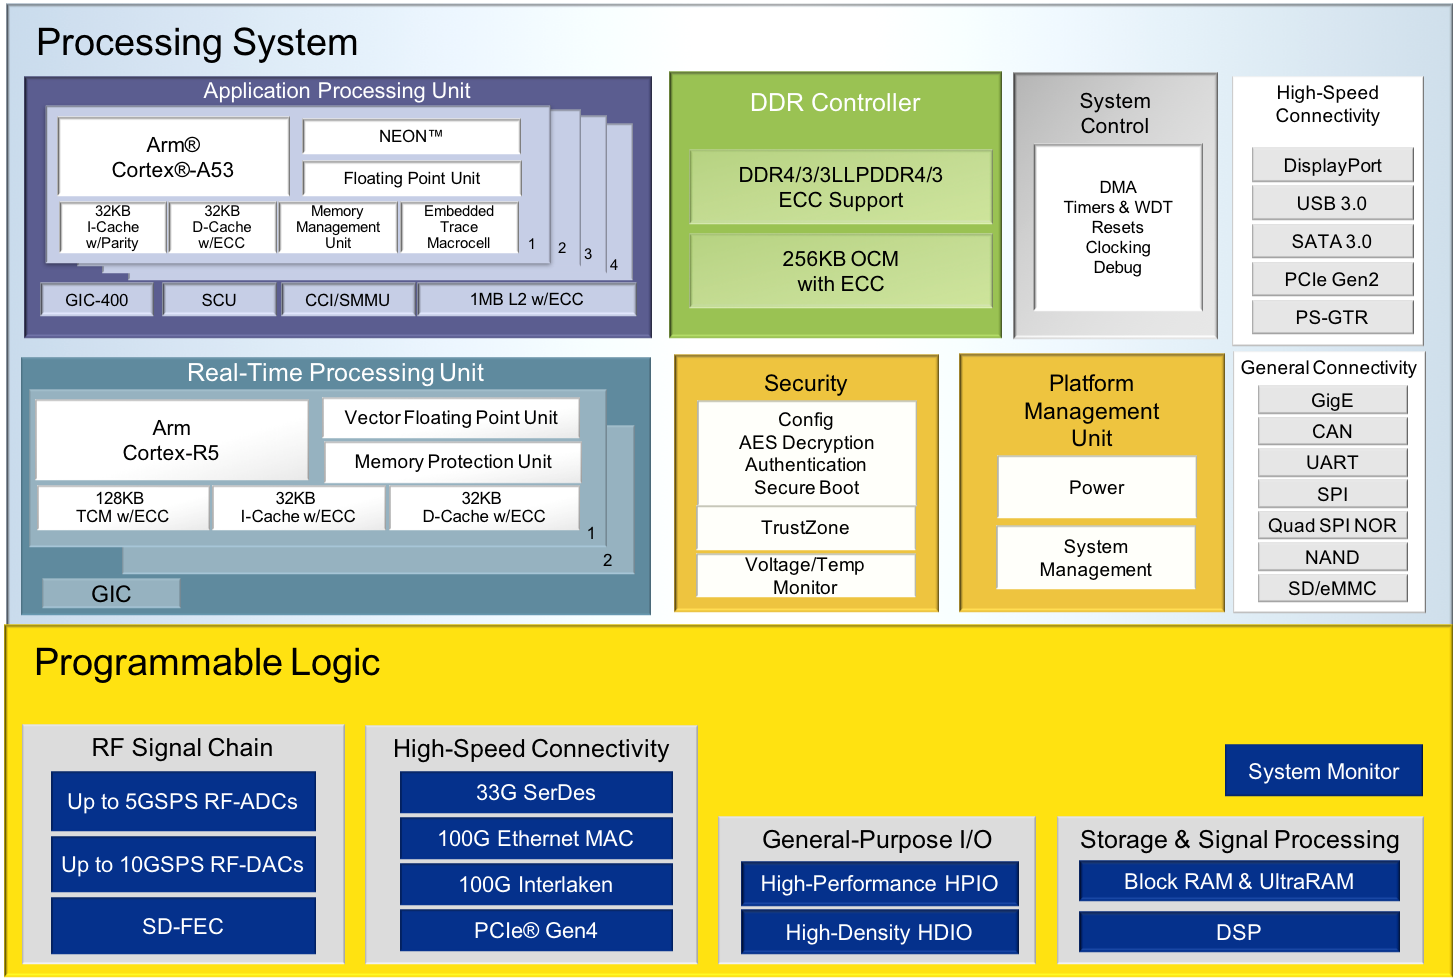
\includegraphics[width = \textwidth]{chap/04-work/img/rfsoc_blockdiagram}
	\caption{RFSoC block diagram}
	\label{fig:rfsoc}
\end{figure}
\paragraph{Evaluation Tool}
\section{Firmware}
\subsection{RF Data Converter}
\subsection{SoC}
\subsection{RDMA over Converged Ethernet (RoCE)}
As its name shows, RoCE is a network protocol defined in the InfiniBand Trade Association (IBTA) standard, allowing RDMA over converged Ethernet network. Shortly, it can be regarded as the application of RDMA technology in hyper-converged data centers, cloud, storage, and virtualized environments. It possesses all the benefits of RDMA technology and the familiarity of Ethernet.

Types of RoCE
Generally, there are two RoCE versions: RoCE v1 and RoCE v2. It depends on the network adapter or card used.

RoCE v1: The RoCE v1 protocol is an Ethernet link layer protocol allowing two hosts in the same Ethernet broadcast domain (VLAN) to communicate. It uses Ethertype 0x8915, which limits the frame length as 1500 bytes for a standard Ethernet frame and 9000 bytes for an Ethernet jumbo frame.

RoCE v2: The RoCE v2 protocol overcomes the limitation of version 1 being bounded to a single broadcast domain (VLAN). By changing the packet encapsulation to include IP and UDP headers, RoCE v2 can now be used across both L2 and L3 networks. This enables Layer 3 routing, which brings RDMA to network with multiple subnets for great scalability. Therefore, RoCE v2 is also regarded as Routable RoCE (RRoCE). Owing to the arrival of RoCE v2, the IP multicast is now also possible.
\subsection{System Integration}


	
	\chapter{Conclusion and Outlook}	
			%\section{Evaluation of the ZCU216 Board/ADCs}
%
%\begin{figure}[H]
%	\centering
%	\includegraphics[width = \textwidth]{chap/05-characterization/img/zcu216evaltool.png}
%	\caption{RF DC Evaluation Tool architecture \cite{zcu216evaltool}}
%	\label{fig:evaltool}
%\end{figure}
%
%
%\subsection{Measurements with Xilinx XM655 add-on card}
%\begin{figure}[H]
%	\centering
%	\includegraphics[width = 0.6\textwidth]{chap/05-characterization/img/evaltool.png}
%	\caption{RF DC Evaluation Tool GUI \cite{zcu216evaltool}}
%	\label{fig:evalgui}
%\end{figure}
%
%
%\begin{figure}[H]
%	\centering
%	\includegraphics[width = 0.7\textwidth]{chap/05-characterization/img/plot1.png}
%	\caption{Placeholder}
%	\label{fig:plot1}
%\end{figure}
%\begin{figure}[H]
%	\centering
%	\includegraphics[width = 0.7\textwidth]{chap/05-characterization/img/plot2.png}
%	\caption{Placeholder}
%	\label{fig:plot2}
%\end{figure}


%\includemedia[	width=\linewidth,
%				height=0.5\linewidth,
%				activate=pageopen,
%				3Dmenu
%				]{}{output.u3d}
	\glsresetall
    \chapter{Conclusion and Outlook}
   			Analysis of events occurring in the range of femtoseconds is desired in many scientific experiments.
The high temporal resolution needed for measuring such events imposes a great technological challenge for \glspl{daq} and \glspl{adc}.
In order to relax the requirements on the acquisition systems, the so-called optical time-stretch technique is used to stretch the analog input signal in time.
In this way, data converters at relatively moderate sample rate can be used.
Measuring the signal with commercial \glspl{daq}, such as real-time oscilloscope, still poses another challenge.
Due to the limited acquisition time windows of such systems, continuous measurements at high sampling rate over long time is not possible.
In applications, where measurements of long-term evolution of the ultra-fast events is desired, this is a major limitation.
Therefore new concepts of \gls{daq} based on the time-stretch method need to be considered in order to overcome this limitation. 

In this thesis, a first demonstrator of such a new \gls{daq} system based on the photonic time-stretch method was developed.
The system consists of a high bandwidth front-end sampling card, mounted on a back-end card integrating a new generation of \gls{rfsoc} for readout of the acquired samples. The name given to the system is \gls{theresa}.

The front-end sampling card integrates 16 sampling channels, each containing a \gls{tha} with individually programmable delay in sampling time. 
The design of the board allows it to be used in two different modes: with and without the time-stretch setup.
In single-channel mode one detector is connected to one sampling channel, therefore allowing sampling of up to 16 detectors at the same time with one sampling point per channel.
In the second mode, several channels are connected to one detector via power splitter, therefore allowing multiple sampling points for one detector/per channel by setting the delay times accordingly. 

High-speed \glspl{adc}, integrated in the \gls{rfsoc}, with 14-bit resolution and a sample rate of up to \SI{2.5}{\giga \sample \per \second} allow continuous sampling of the signal with high time resolution. 
Using the time-interleaving technique for all sixteen \glspl{adc} results in an overall maximal achievable sample rate of \SI{40}{\giga \sample \per \second} possible.  
When using in combination with the time-stretch technique and considering typical stretch-factors, these \SI{11}{\pico \second} are translated into a range of femtoseconds in the original signal.

The sampling card was furthermore designed to fully exploit all the features of the \gls{rfsoc}, which integrates a processing unit together with a \gls{fpga}.
An evaluation tool framework is provided for the selected read-out card, allowing for on-board data generation and capture.
This tool was also evaluated; allowing for quick set-up and measurement of key data converter characteristics (\gls{sinad}, \gls{sfdr}, ...) it provides an invaluable tool in order to get a first impression of the performance of the sampling card.

The on-chip \gls{fpga} provides the possibility to flexibly adjust the firmware to user needs. 
Slow-control implemented in the \gls{fpga} takes care of programming the components on the sampling card, such as the delay chips.
High-speed interfaces, allowing speeds over 100 Gb/s, are a crucial component for the high throughput of the large amount of data generated by the data converters; with the given resolution and max. sample rate this touches the range of TB/s.


The design of the sampling card was approved and the card has been deployed in production.
Quick characterization of the card is possible due to the tool deployed on the redout-card and can be carried out using the methods described in \autoref{ssec:adc_charac}.
\gls{theresa} can then be commissioned and taken into operation, improving theresearch in various scientific fields, especially beam diagnostics at e.g. \gls{kara}. 
There it can be used for studying \gls{csr}, in the far-field and near-field electro-optic setup, for study of fast laser dynamics and many other applications.
The selected \gls{fpga} is suitable for deploying Artificial Intelligence applications (i.e. Reinforcement Learning).
Therefore the system can also be used for interfacing with the BBB feedback at \gls{kara}.
In the context of the ULTRASYNC project, funded by ANR-DFG, \gls{theresa} can be used in order to study the control of electron bunches in accelerators at \gls{kara} and SOLEIL, therefore being an important step towards new usable \gls{thz} sources. 
 

%There is a disturbing lack of benches in \sout{Ramset Park} Campus North. I want to sit more!
%
%\begin{figure}[tbh]
%	\includegraphics[width=\textwidth]{chap/06-conclusion/img/april}
%\end{figure}
%
%\newpage
%\section{Expectation vs. Reality}
%At least I wrote more than 273 words.
%\begin{figure}[tbh]
%     \centering
%     \begin{subfigure}{0.7\textwidth}
%         \centering
%         \includegraphics[width=\textwidth]{chap/06-conclusion/img/harper}
%         \caption{How you think you will feel like at the end of your master studies.}
%         \label{fig:expectation}
%     \end{subfigure}
%     
%     \begin{subfigure}{0.7\textwidth}
%         \centering
%         \includegraphics[width=\textwidth]{chap/06-conclusion/img/bubi}
%         \caption{How you actually feel like.}
%         \label{fig:reality}
%     \end{subfigure}
%     \caption{Expectation vs. Reality}
%\end{figure}
%
%
%
%\section{The board}
%\begin{figure}[H]
%	\centering
%	\includegraphics[width = \textwidth]{chap/06-conclusion/img/board}
%	\caption{THERESA}
%	\label{fig:board}
%\end{figure}
		
	\chapter*{Acknowledgments}\addcontentsline{toc}{chapter}{Acknowledgements}
			First, I would like to thank Prof. Anke-Susanne Müller from the Institute of Beam Physics and Technology for being my first reviewer.

I want to express my sincere appreciation for my advisor Dr. Michele Caselle for always being a great support and an excellent teacher, who always has time to explain all details, even if it concerns fundamental topics. 
His great support at all times made the successful conclusion of this thesis and my studies possible.

Prof. Serge Bielawski from Lille University I would like to thank for the collaboration and the useful feedback concerning the system.

I would also like to thank Andreas Kopmann (IPE) for his support during the writing of this thesis and the preparation of the final defence.

Michael Schleicher (IPE) I would like to thank for his useful advice and help during the design phase of the card layout.

My biggest gratitude also goes to Meghana Patil (LAS)  for her support at all times, especially during the last phase of writing and preparation of my presentation.

I would like to thank Miriam Brosi (IBPT) for giving me the possibility to see the KARA facility from inside and for prove-reading my t the physics part of hesis.

I am eternally grateful to Marvin Noll for his invaluable support not only during the writing of the thesis (especially concerning LaTeX-related questions) and the preparation of the final defense, but also for his great support at any times during the whole course of my studies.

Finally, I would like to thank my parents for always supporting me in any situations at all times. I owe them my biggest appreciation for successfully completing my studies, without their support and care this would have never been possible.

	
    \Appendix
    \chapter*{\appendixname} \addcontentsline{toc}{chapter}{\appendixname}
    		\section{Characteristic Impedance Of Coplanar Waveguides} \label{app:waveguides}
\paragraph{Edge-Coupled Coplanar Waveguide}

Characteristic impedance (see \cite[~p197-198]{wadell}): 
\begin{align}
	Z_{0,o} &= \frac{\eta_0}{\sqrt{\epsilon_{\text{eff},o}}} \left( \frac{1.0}{2.0 \frac{K(k_o)}{K'(k_o)} + \frac{K(\beta_1)}{K'(\beta_1)}}\right)\\
	Z_{0,e} &= \frac{\eta_0}{\sqrt{\epsilon_{\text{eff},e}}} \left( \frac{1.0}{2.0 \frac{K(k_e)}{K'(k_e)} + \frac{K(\beta_1 k_1)}{K'(\beta_1 k_1)}}\right)
\end{align}    

\begin{align}
	\epsilon_{\text{eff},o} &= \frac{2.0 \epsilon_r \frac{K(k_o)}{K'(k_o)} + \frac{K(\beta_1)}{K'(\beta_1)}}{2.0 \frac{K(k_o)}{K'(k_o)} + \frac{K(\beta_1)}{K'(\beta_1)}}\\
	\epsilon_{\text{eff},e} &= \frac{2.0 \epsilon_r \frac{K(k_e)}{K'(k_e)} + \frac{K(\beta_1 k_1)}{K'(\beta_1 k_1)}}{2.0 \frac{K(k_e)}{K'(k_e)} + \frac{K(\beta_1 k_1)}{K'(\beta_1 k_1)}}
\end{align}

with

\begin{align}
	k_o &= \Lambda \frac{-\sqrt{\Lambda^2 - t_c^2} + \sqrt{\Lambda^2 - t_B^2}}{t_B\sqrt{\Lambda^2 - t_c^2} + t_c \sqrt{\Lambda^2 - t_B^2}}\\
	k_e &= \Lambda' \frac{-\sqrt{\Lambda'^2 - t_c'^2} + \sqrt{\Lambda'^2 - t_B'^2}}{t_B'\sqrt{\Lambda'^2 - t_c'^2} + t_c' \sqrt{\Lambda'^2 - t_B'^2}}
\end{align}


\begin{equation}
	\Lambda = \frac{\sinh^2 \left( \frac{\pi (s/2.0 + w + d)}{2.0 h} \right) }{2}
\end{equation}

\begin{equation}
	t_c = \sinh^2 \left( \frac{\pi (s/2.0 + w)}{2.0 h} \right) - \Lambda
\end{equation}

\begin{equation}
	t_B = \sinh^2 \left( \frac{\pi s}{4.0 h} \right) - \Lambda
\end{equation}


\begin{equation}
	\Lambda' = \frac{\cosh^2 \left( \frac{\pi (s/2.0 + w + d)}{2.0 h} \right) }{2}
\end{equation}

\begin{equation}
	t_c' = \sinh^2 \left( \frac{\pi (s/2.0 + w)}{2.0 h} \right) - \Lambda' + 1.0
\end{equation}

\begin{equation}
	t_B' = \sinh^2 \left( \frac{\pi s}{4.0 h} \right) - \Lambda + 1.0
\end{equation}

The parameters have to be chosen according to 
\begin{equation}
	s + 2.0 w + 2.0 d \leq h
\end{equation}
to guarantee coplanar propagation. \cite{wadell}


\paragraph{Surface Coplanar Waveguide with Ground}  
The characteristic impedance of a coplanar waveguide is given as (see \cite{wadell}) 
\begin{equation}
	Z_0 = \frac{60.0 \pi}{\sqrt{\epsilon_\text{eff}}} \frac{1.0}{\frac{K(k)}{K(k')} + \frac{K(k_1)}{K(k_1')}}.
\end{equation}
It comprises of the following components, with $K(k)$ being an elliptical integral of the first kind (see also \cite[p.~430]{bronstein}):
\begin{align}
	k &= a/b\\
	k' &= \sqrt{1.0 - k^{2}}\\
	k_1 &= \frac{\tanh(\frac{\pi a}{4.0  h})}{\tanh(\frac{\pi  b}{4.0 h})}\\
	k_1' &= \sqrt{1.0 - k_1^{2}}\\
	\epsilon_\text{eff} &= \frac{1.0 + \epsilon_r \frac{K(k')}{K(k)} \frac{K(k_1)}{K(k_1')}}{1.0 + \frac{K(k')}{K(k)} \frac{K(k_1)}{K(k_1')}}
\end{align}

\section{Verilog Code for SPI Interface For Delay Chips} \label{app:code} %todo what code?
\lstinputlisting[language=Verilog, basicstyle=\footnotesize]{chap/07-appendix/include/delayfirmware.v}
%todo add linebreaks to the lstlisting style


	\TheBibliography
	\bibliographystyle{babalpha}
	\bibliography{lit}
\end{document}
